\documentclass{book}
\usepackage[a4paper,top=2.5cm,bottom=2.5cm,left=2.5cm,right=2.5cm]{geometry}
\usepackage{makeidx}
\usepackage{natbib}
\usepackage{graphicx}
\usepackage{multicol}
\usepackage{float}
\usepackage{listings}
\usepackage{color}
\usepackage{ifthen}
\usepackage[table]{xcolor}
\usepackage{textcomp}
\usepackage{alltt}
\usepackage{ifpdf}
\ifpdf
\usepackage[pdftex,
            pagebackref=true,
            colorlinks=true,
            linkcolor=blue,
            unicode
           ]{hyperref}
\else
\usepackage[ps2pdf,
            pagebackref=true,
            colorlinks=true,
            linkcolor=blue,
            unicode
           ]{hyperref}
\usepackage{pspicture}
\fi
\usepackage[utf8]{inputenc}
\usepackage[ngerman]{babel}

\usepackage{mathptmx}
\usepackage[scaled=.90]{helvet}
\usepackage{courier}
\usepackage{sectsty}
\usepackage{amssymb}
\usepackage[titles]{tocloft}
\usepackage{doxygen}
\lstset{language=C++,inputencoding=utf8,basicstyle=\footnotesize,breaklines=true,breakatwhitespace=true,tabsize=4,numbers=left }
\makeindex
\setcounter{tocdepth}{3}
\renewcommand{\footrulewidth}{0.4pt}
\renewcommand{\familydefault}{\sfdefault}
\hfuzz=15pt
\setlength{\emergencystretch}{15pt}
\hbadness=750
\tolerance=750
\begin{document}
\hypersetup{pageanchor=false,citecolor=blue}
\begin{titlepage}
\vspace*{7cm}
\begin{center}
{\Large gruppe\-B4 Entwicklerdokumentation }\\
\vspace*{1cm}
{\large Erzeugt von Doxygen 1.8.3.1}\\
\vspace*{0.5cm}
{\small Son Jul 7 2013 10:54:59}\\
\end{center}
\end{titlepage}
\clearemptydoublepage
\pagenumbering{roman}
\tableofcontents
\clearemptydoublepage
\pagenumbering{arabic}
\hypersetup{pageanchor=true,citecolor=blue}
\chapter{Hierarchie-\/\-Verzeichnis}
\section{Klassenhierarchie}
Die Liste der Ableitungen ist -\/mit Einschränkungen-\/ alphabetisch sortiert\-:\begin{DoxyCompactList}
\item \contentsline{section}{Actor}{\pageref{class_actor}}{}
\item \contentsline{section}{Agent\-Manager}{\pageref{class_agent_manager}}{}
\item \contentsline{section}{Armor}{\pageref{class_armor}}{}
\item \contentsline{section}{Armor\-Manager}{\pageref{class_armor_manager}}{}
\item \contentsline{section}{Enemy}{\pageref{class_enemy}}{}
\begin{DoxyCompactList}
\item \contentsline{section}{Crazy\-\_\-enemy}{\pageref{class_crazy__enemy}}{}
\item \contentsline{section}{Crazy\-\_\-enemy}{\pageref{class_crazy__enemy}}{}
\item \contentsline{section}{Endboss}{\pageref{class_endboss}}{}
\end{DoxyCompactList}
\item \contentsline{section}{E\-P\-Manager}{\pageref{class_e_p_manager}}{}
\item \contentsline{section}{Final\-Boss}{\pageref{class_final_boss}}{}
\item \contentsline{section}{Item}{\pageref{class_item}}{}
\item \contentsline{section}{Item\-Manager}{\pageref{class_item_manager}}{}
\item \contentsline{section}{Level\-Segmente}{\pageref{class_level_segmente}}{}
\item \contentsline{section}{Main\-\_\-\-Menue}{\pageref{class_main___menue}}{}
\item \contentsline{section}{Menue}{\pageref{class_menue}}{}
\item \contentsline{section}{Money\-Manager}{\pageref{class_money_manager}}{}
\item \contentsline{section}{N\-P\-C1}{\pageref{class_n_p_c1}}{}
\item \contentsline{section}{N\-P\-C2}{\pageref{class_n_p_c2}}{}
\item \contentsline{section}{N\-P\-C\-Manager}{\pageref{class_n_p_c_manager}}{}
\item \contentsline{section}{Overlay}{\pageref{class_overlay}}{}
\item \contentsline{section}{Pfleger}{\pageref{class_pfleger}}{}
\item \contentsline{section}{Player}{\pageref{class_player}}{}
\item \contentsline{section}{Player2}{\pageref{class_player2}}{}
\item \contentsline{section}{Renable\-Object}{\pageref{class_renable_object}}{}
\item \contentsline{section}{S\-\_\-\-Resourcemanager}{\pageref{class_s___resourcemanager}}{}
\item \contentsline{section}{s\-\_\-\-Vector}{\pageref{structs___vector}}{}
\item \contentsline{section}{Shop}{\pageref{class_shop}}{}
\item \contentsline{section}{Skilltree}{\pageref{class_skilltree}}{}
\item \contentsline{section}{Spritze}{\pageref{class_spritze}}{}
\item \contentsline{section}{Timer}{\pageref{class_timer}}{}
\item \contentsline{section}{Weapon\-Manager}{\pageref{class_weapon_manager}}{}
\item \contentsline{section}{World}{\pageref{class_world}}{}
\end{DoxyCompactList}

\chapter{Klassen-\/\-Verzeichnis}
\section{Auflistung der Klassen}
Hier folgt die Aufzählung aller Klassen, Strukturen, Varianten und Schnittstellen mit einer Kurzbeschreibung\-:\begin{DoxyCompactList}
\item\contentsline{section}{\hyperlink{class_actor}{Actor} }{\pageref{class_actor}}{}
\item\contentsline{section}{\hyperlink{class_agent_manager}{Agent\-Manager} }{\pageref{class_agent_manager}}{}
\item\contentsline{section}{\hyperlink{class_armor}{Armor} }{\pageref{class_armor}}{}
\item\contentsline{section}{\hyperlink{class_armor_manager}{Armor\-Manager} }{\pageref{class_armor_manager}}{}
\item\contentsline{section}{\hyperlink{class_crazy__enemy}{Crazy\-\_\-enemy} }{\pageref{class_crazy__enemy}}{}
\item\contentsline{section}{\hyperlink{class_endboss}{Endboss} }{\pageref{class_endboss}}{}
\item\contentsline{section}{\hyperlink{class_enemy}{Enemy} }{\pageref{class_enemy}}{}
\item\contentsline{section}{\hyperlink{class_e_p_manager}{E\-P\-Manager} }{\pageref{class_e_p_manager}}{}
\item\contentsline{section}{\hyperlink{class_final_boss}{Final\-Boss} }{\pageref{class_final_boss}}{}
\item\contentsline{section}{\hyperlink{class_item}{Item} }{\pageref{class_item}}{}
\item\contentsline{section}{\hyperlink{class_item_manager}{Item\-Manager} }{\pageref{class_item_manager}}{}
\item\contentsline{section}{\hyperlink{class_level_segmente}{Level\-Segmente} }{\pageref{class_level_segmente}}{}
\item\contentsline{section}{\hyperlink{class_main___menue}{Main\-\_\-\-Menue} }{\pageref{class_main___menue}}{}
\item\contentsline{section}{\hyperlink{class_menue}{Menue} }{\pageref{class_menue}}{}
\item\contentsline{section}{\hyperlink{class_money_manager}{Money\-Manager} }{\pageref{class_money_manager}}{}
\item\contentsline{section}{\hyperlink{class_n_p_c1}{N\-P\-C1} }{\pageref{class_n_p_c1}}{}
\item\contentsline{section}{\hyperlink{class_n_p_c2}{N\-P\-C2} }{\pageref{class_n_p_c2}}{}
\item\contentsline{section}{\hyperlink{class_n_p_c_manager}{N\-P\-C\-Manager} }{\pageref{class_n_p_c_manager}}{}
\item\contentsline{section}{\hyperlink{class_overlay}{Overlay} }{\pageref{class_overlay}}{}
\item\contentsline{section}{\hyperlink{class_pfleger}{Pfleger} }{\pageref{class_pfleger}}{}
\item\contentsline{section}{\hyperlink{class_player}{Player} }{\pageref{class_player}}{}
\item\contentsline{section}{\hyperlink{class_player2}{Player2} }{\pageref{class_player2}}{}
\item\contentsline{section}{\hyperlink{class_renable_object}{Renable\-Object} }{\pageref{class_renable_object}}{}
\item\contentsline{section}{\hyperlink{class_s___resourcemanager}{S\-\_\-\-Resourcemanager} }{\pageref{class_s___resourcemanager}}{}
\item\contentsline{section}{\hyperlink{structs___vector}{s\-\_\-\-Vector} }{\pageref{structs___vector}}{}
\item\contentsline{section}{\hyperlink{class_shop}{Shop} }{\pageref{class_shop}}{}
\item\contentsline{section}{\hyperlink{class_skilltree}{Skilltree} }{\pageref{class_skilltree}}{}
\item\contentsline{section}{\hyperlink{class_spritze}{Spritze} }{\pageref{class_spritze}}{}
\item\contentsline{section}{\hyperlink{class_timer}{Timer} }{\pageref{class_timer}}{}
\item\contentsline{section}{\hyperlink{class_weapon_manager}{Weapon\-Manager} }{\pageref{class_weapon_manager}}{}
\item\contentsline{section}{\hyperlink{class_world}{World} }{\pageref{class_world}}{}
\end{DoxyCompactList}

\chapter{Klassen-\/\-Dokumentation}
\hypertarget{class_actor}{\section{Actor Klassenreferenz}
\label{class_actor}\index{Actor@{Actor}}
}


{\ttfamily \#include $<$Actor.\-h$>$}



Zusammengehörigkeiten von Actor\-:
\nopagebreak
\begin{figure}[H]
\begin{center}
\leavevmode
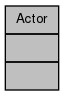
\includegraphics[width=162pt]{class_actor__coll__graph}
\end{center}
\end{figure}
\subsection*{Private Methoden}
\begin{DoxyCompactItemize}
\item 
virtual void \hyperlink{class_actor_ae0bbd128243b28cdbed179647515f693}{get\-\_\-\-Position} ()=0
\item 
virtual void \hyperlink{class_actor_ae398ba9911fa9a43cf237c4e87d6e047}{set\-\_\-\-Position} ()=0
\end{DoxyCompactItemize}


\subsection{Dokumentation der Elementfunktionen}
\hypertarget{class_actor_ae0bbd128243b28cdbed179647515f693}{\index{Actor@{Actor}!get\-\_\-\-Position@{get\-\_\-\-Position}}
\index{get\-\_\-\-Position@{get\-\_\-\-Position}!Actor@{Actor}}
\subsubsection[{get\-\_\-\-Position}]{\setlength{\rightskip}{0pt plus 5cm}virtual void Actor\-::get\-\_\-\-Position (
\begin{DoxyParamCaption}
{}
\end{DoxyParamCaption}
)\hspace{0.3cm}{\ttfamily [private]}, {\ttfamily [pure virtual]}}}\label{class_actor_ae0bbd128243b28cdbed179647515f693}
\hypertarget{class_actor_ae398ba9911fa9a43cf237c4e87d6e047}{\index{Actor@{Actor}!set\-\_\-\-Position@{set\-\_\-\-Position}}
\index{set\-\_\-\-Position@{set\-\_\-\-Position}!Actor@{Actor}}
\subsubsection[{set\-\_\-\-Position}]{\setlength{\rightskip}{0pt plus 5cm}virtual void Actor\-::set\-\_\-\-Position (
\begin{DoxyParamCaption}
{}
\end{DoxyParamCaption}
)\hspace{0.3cm}{\ttfamily [private]}, {\ttfamily [pure virtual]}}}\label{class_actor_ae398ba9911fa9a43cf237c4e87d6e047}


Die Dokumentation für diese Klasse wurde erzeugt aufgrund der Datei\-:\begin{DoxyCompactItemize}
\item 
\hyperlink{_actor_8h}{Actor.\-h}\end{DoxyCompactItemize}

\hypertarget{class_agent_manager}{\section{Agent\-Manager Klassenreferenz}
\label{class_agent_manager}\index{Agent\-Manager@{Agent\-Manager}}
}


{\ttfamily \#include $<$Agent\-Manager.\-h$>$}



Zusammengehörigkeiten von Agent\-Manager\-:
\nopagebreak
\begin{figure}[H]
\begin{center}
\leavevmode
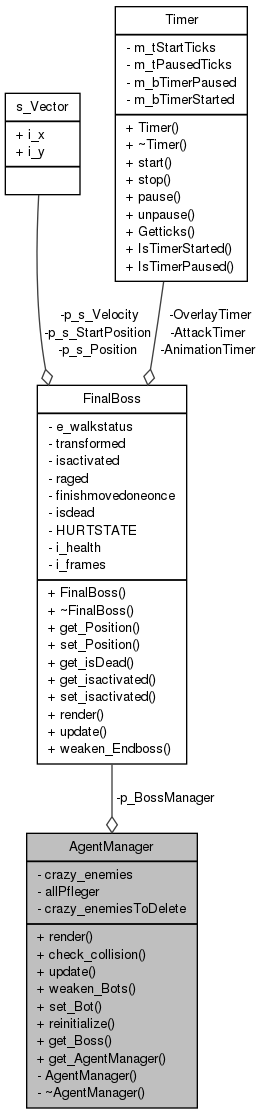
\includegraphics[height=550pt]{class_agent_manager__coll__graph}
\end{center}
\end{figure}
\subsection*{Öffentliche Methoden}
\begin{DoxyCompactItemize}
\item 
void \hyperlink{class_agent_manager_a1b94eb002a1a9a57106539b84402f32a}{render} (S\-D\-L\-\_\-\-Rect camera, \hyperlink{globals_8h_a3951bd57665e2e4c8a4411c2a5477207}{L\-E\-V\-E\-L\-\_\-\-L\-O\-A\-D\-E\-D} T\-E\-M\-P\-L\-E\-V\-E\-L)
\item 
void \hyperlink{class_agent_manager_a5548da9e3f247e8dd4a9eb98748fd3df}{check\-\_\-collision} (\hyperlink{class_player}{Player} $\ast$p\-\_\-\-Temp\-Player, int durchlaufvariable)
\item 
void \hyperlink{class_agent_manager_a1c05e1578aafde1892a5e4e79862b19f}{update} (\hyperlink{class_player}{Player} $\ast$p\-\_\-\-Temp\-Player, \hyperlink{globals_8h_a3951bd57665e2e4c8a4411c2a5477207}{L\-E\-V\-E\-L\-\_\-\-L\-O\-A\-D\-E\-D}, S\-D\-L\-\_\-\-Rect camera)
\item 
void \hyperlink{class_agent_manager_aafa2ae19bfa65b44dc3c955bd21e0fc3}{weaken\-\_\-\-Bots} (\hyperlink{class_player}{Player} $\ast$p\-\_\-\-Temp\-Player)
\item 
void \hyperlink{class_agent_manager_ab00a9cbf5753546fbb5f9f5cfa1b1241}{set\-\_\-\-Bot} (int x, int y, \hyperlink{globals_8h_aaf436d1bc29db707b62c299461f32ee7}{B\-O\-T\-\_\-\-T\-Y\-P\-E} T\-E\-M\-P\-T\-Y\-P\-E)
\item 
void \hyperlink{class_agent_manager_abc1499700649f6af77205fedc0698085}{reinitialize} ()
\item 
\hyperlink{class_final_boss}{Final\-Boss} $\ast$ \hyperlink{class_agent_manager_a13afeaa1a5581415e3b312444bb43b82}{get\-\_\-\-Boss} ()
\end{DoxyCompactItemize}
\subsection*{Öffentliche, statische Methoden}
\begin{DoxyCompactItemize}
\item 
static \hyperlink{class_agent_manager}{Agent\-Manager} \& \hyperlink{class_agent_manager_a1af0e6f1ed0b2b4db25617f4e9357e81}{get\-\_\-\-Agent\-Manager} ()
\end{DoxyCompactItemize}
\subsection*{Private Methoden}
\begin{DoxyCompactItemize}
\item 
\hyperlink{class_agent_manager_a49ff5a8f60bae1c0b8d6c9aeda8f6961}{Agent\-Manager} ()
\item 
\hyperlink{class_agent_manager_a6b3efb95b74c9c96b9dbaf0868f17759}{$\sim$\-Agent\-Manager} ()
\end{DoxyCompactItemize}
\subsection*{Private Attribute}
\begin{DoxyCompactItemize}
\item 
vector$<$ \hyperlink{class_crazy__enemy}{Crazy\-\_\-enemy} $\ast$ $>$ \hyperlink{class_agent_manager_a3a921dcdcad9845bb40ec0cf67b6cd2e}{crazy\-\_\-enemies}
\begin{DoxyCompactList}\small\item\em Vektor der alle Crazy enemies speichert. \end{DoxyCompactList}\item 
vector$<$ \hyperlink{class_pfleger}{Pfleger} $\ast$ $>$ \hyperlink{class_agent_manager_a1c7aff8c522d35fd1514eb953195be92}{all\-Pfleger}
\item 
vector$<$ \hyperlink{class_crazy__enemy}{Crazy\-\_\-enemy} $\ast$ $>$ \hyperlink{class_agent_manager_ad04668952fb54954caf87f088eedf4ca}{crazy\-\_\-enemies\-To\-Delete}
\item 
\hyperlink{class_final_boss}{Final\-Boss} $\ast$ \hyperlink{class_agent_manager_a44183c7f9aa95bfdfab8e2c075d530a3}{p\-\_\-\-Boss\-Manager}
\end{DoxyCompactItemize}


\subsection{Beschreibung der Konstruktoren und Destruktoren}
\hypertarget{class_agent_manager_a49ff5a8f60bae1c0b8d6c9aeda8f6961}{\index{Agent\-Manager@{Agent\-Manager}!Agent\-Manager@{Agent\-Manager}}
\index{Agent\-Manager@{Agent\-Manager}!AgentManager@{Agent\-Manager}}
\subsubsection[{Agent\-Manager}]{\setlength{\rightskip}{0pt plus 5cm}Agent\-Manager\-::\-Agent\-Manager (
\begin{DoxyParamCaption}
{}
\end{DoxyParamCaption}
)\hspace{0.3cm}{\ttfamily [inline]}, {\ttfamily [private]}}}\label{class_agent_manager_a49ff5a8f60bae1c0b8d6c9aeda8f6961}
\hypertarget{class_agent_manager_a6b3efb95b74c9c96b9dbaf0868f17759}{\index{Agent\-Manager@{Agent\-Manager}!$\sim$\-Agent\-Manager@{$\sim$\-Agent\-Manager}}
\index{$\sim$\-Agent\-Manager@{$\sim$\-Agent\-Manager}!AgentManager@{Agent\-Manager}}
\subsubsection[{$\sim$\-Agent\-Manager}]{\setlength{\rightskip}{0pt plus 5cm}Agent\-Manager\-::$\sim$\-Agent\-Manager (
\begin{DoxyParamCaption}
{}
\end{DoxyParamCaption}
)\hspace{0.3cm}{\ttfamily [inline]}, {\ttfamily [private]}}}\label{class_agent_manager_a6b3efb95b74c9c96b9dbaf0868f17759}


\subsection{Dokumentation der Elementfunktionen}
\hypertarget{class_agent_manager_a5548da9e3f247e8dd4a9eb98748fd3df}{\index{Agent\-Manager@{Agent\-Manager}!check\-\_\-collision@{check\-\_\-collision}}
\index{check\-\_\-collision@{check\-\_\-collision}!AgentManager@{Agent\-Manager}}
\subsubsection[{check\-\_\-collision}]{\setlength{\rightskip}{0pt plus 5cm}void Agent\-Manager\-::check\-\_\-collision (
\begin{DoxyParamCaption}
\item[{{\bf Player} $\ast$}]{p\-\_\-\-Temp\-Player, }
\item[{int}]{durchlaufvariable}
\end{DoxyParamCaption}
)}}\label{class_agent_manager_a5548da9e3f247e8dd4a9eb98748fd3df}


Hier ist ein Graph, der zeigt, was diese Funktion aufruft\-:\nopagebreak
\begin{figure}[H]
\begin{center}
\leavevmode
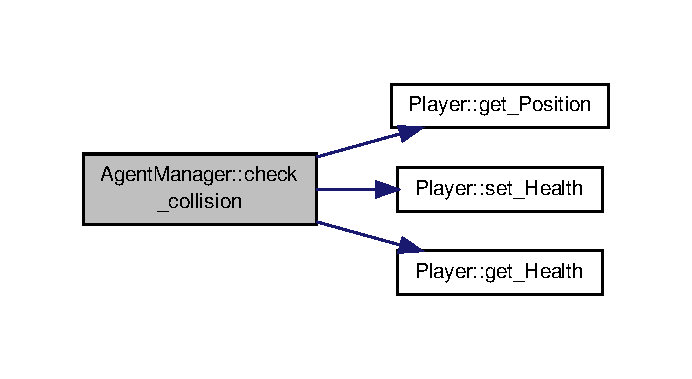
\includegraphics[width=332pt]{class_agent_manager_a5548da9e3f247e8dd4a9eb98748fd3df_cgraph}
\end{center}
\end{figure}




Hier ist ein Graph der zeigt, wo diese Funktion aufgerufen wird\-:\nopagebreak
\begin{figure}[H]
\begin{center}
\leavevmode
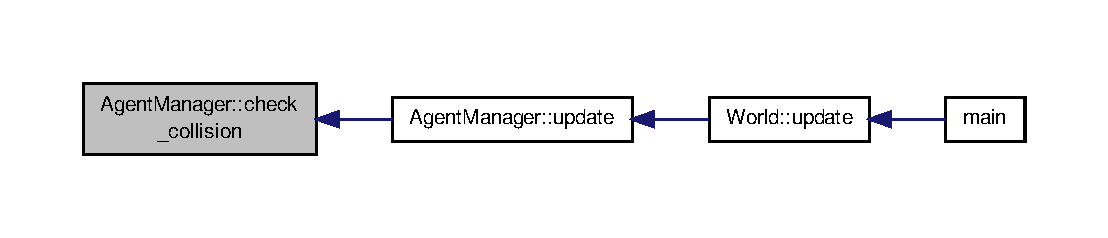
\includegraphics[width=350pt]{class_agent_manager_a5548da9e3f247e8dd4a9eb98748fd3df_icgraph}
\end{center}
\end{figure}


\hypertarget{class_agent_manager_a1af0e6f1ed0b2b4db25617f4e9357e81}{\index{Agent\-Manager@{Agent\-Manager}!get\-\_\-\-Agent\-Manager@{get\-\_\-\-Agent\-Manager}}
\index{get\-\_\-\-Agent\-Manager@{get\-\_\-\-Agent\-Manager}!AgentManager@{Agent\-Manager}}
\subsubsection[{get\-\_\-\-Agent\-Manager}]{\setlength{\rightskip}{0pt plus 5cm}static {\bf Agent\-Manager}\& Agent\-Manager\-::get\-\_\-\-Agent\-Manager (
\begin{DoxyParamCaption}
{}
\end{DoxyParamCaption}
)\hspace{0.3cm}{\ttfamily [inline]}, {\ttfamily [static]}}}\label{class_agent_manager_a1af0e6f1ed0b2b4db25617f4e9357e81}


Hier ist ein Graph der zeigt, wo diese Funktion aufgerufen wird\-:\nopagebreak
\begin{figure}[H]
\begin{center}
\leavevmode
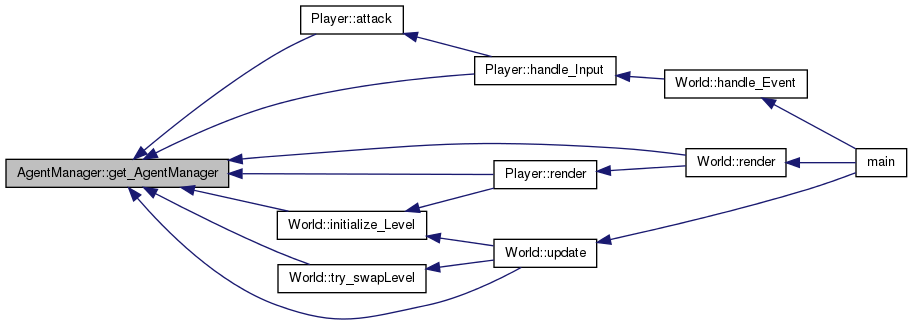
\includegraphics[width=350pt]{class_agent_manager_a1af0e6f1ed0b2b4db25617f4e9357e81_icgraph}
\end{center}
\end{figure}


\hypertarget{class_agent_manager_a13afeaa1a5581415e3b312444bb43b82}{\index{Agent\-Manager@{Agent\-Manager}!get\-\_\-\-Boss@{get\-\_\-\-Boss}}
\index{get\-\_\-\-Boss@{get\-\_\-\-Boss}!AgentManager@{Agent\-Manager}}
\subsubsection[{get\-\_\-\-Boss}]{\setlength{\rightskip}{0pt plus 5cm}{\bf Final\-Boss}$\ast$ Agent\-Manager\-::get\-\_\-\-Boss (
\begin{DoxyParamCaption}
{}
\end{DoxyParamCaption}
)\hspace{0.3cm}{\ttfamily [inline]}}}\label{class_agent_manager_a13afeaa1a5581415e3b312444bb43b82}


Hier ist ein Graph der zeigt, wo diese Funktion aufgerufen wird\-:\nopagebreak
\begin{figure}[H]
\begin{center}
\leavevmode
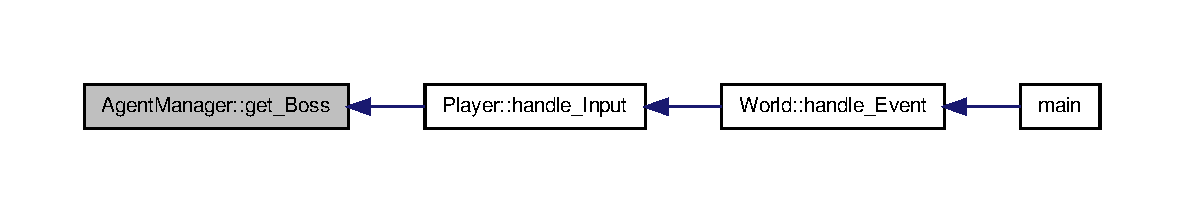
\includegraphics[width=350pt]{class_agent_manager_a13afeaa1a5581415e3b312444bb43b82_icgraph}
\end{center}
\end{figure}


\hypertarget{class_agent_manager_abc1499700649f6af77205fedc0698085}{\index{Agent\-Manager@{Agent\-Manager}!reinitialize@{reinitialize}}
\index{reinitialize@{reinitialize}!AgentManager@{Agent\-Manager}}
\subsubsection[{reinitialize}]{\setlength{\rightskip}{0pt plus 5cm}void Agent\-Manager\-::reinitialize (
\begin{DoxyParamCaption}
{}
\end{DoxyParamCaption}
)\hspace{0.3cm}{\ttfamily [inline]}}}\label{class_agent_manager_abc1499700649f6af77205fedc0698085}


Hier ist ein Graph der zeigt, wo diese Funktion aufgerufen wird\-:\nopagebreak
\begin{figure}[H]
\begin{center}
\leavevmode
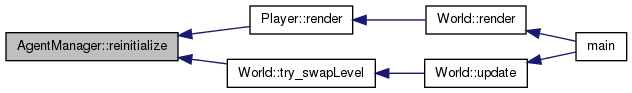
\includegraphics[width=350pt]{class_agent_manager_abc1499700649f6af77205fedc0698085_icgraph}
\end{center}
\end{figure}


\hypertarget{class_agent_manager_a1b94eb002a1a9a57106539b84402f32a}{\index{Agent\-Manager@{Agent\-Manager}!render@{render}}
\index{render@{render}!AgentManager@{Agent\-Manager}}
\subsubsection[{render}]{\setlength{\rightskip}{0pt plus 5cm}void Agent\-Manager\-::render (
\begin{DoxyParamCaption}
\item[{S\-D\-L\-\_\-\-Rect}]{camera, }
\item[{{\bf L\-E\-V\-E\-L\-\_\-\-L\-O\-A\-D\-E\-D}}]{T\-E\-M\-P\-L\-E\-V\-E\-L}
\end{DoxyParamCaption}
)}}\label{class_agent_manager_a1b94eb002a1a9a57106539b84402f32a}


Hier ist ein Graph, der zeigt, was diese Funktion aufruft\-:\nopagebreak
\begin{figure}[H]
\begin{center}
\leavevmode
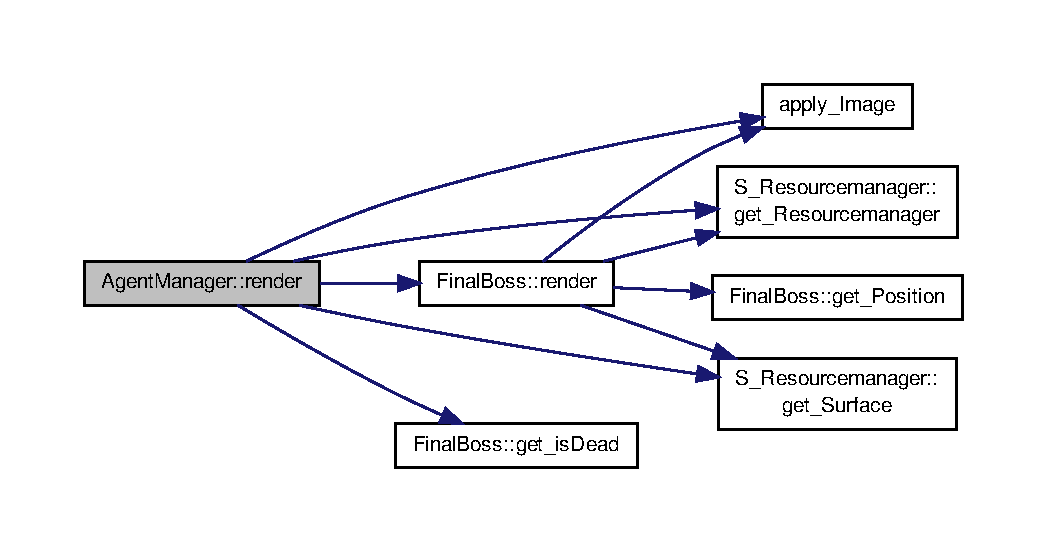
\includegraphics[width=350pt]{class_agent_manager_a1b94eb002a1a9a57106539b84402f32a_cgraph}
\end{center}
\end{figure}




Hier ist ein Graph der zeigt, wo diese Funktion aufgerufen wird\-:\nopagebreak
\begin{figure}[H]
\begin{center}
\leavevmode
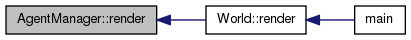
\includegraphics[width=350pt]{class_agent_manager_a1b94eb002a1a9a57106539b84402f32a_icgraph}
\end{center}
\end{figure}


\hypertarget{class_agent_manager_ab00a9cbf5753546fbb5f9f5cfa1b1241}{\index{Agent\-Manager@{Agent\-Manager}!set\-\_\-\-Bot@{set\-\_\-\-Bot}}
\index{set\-\_\-\-Bot@{set\-\_\-\-Bot}!AgentManager@{Agent\-Manager}}
\subsubsection[{set\-\_\-\-Bot}]{\setlength{\rightskip}{0pt plus 5cm}void Agent\-Manager\-::set\-\_\-\-Bot (
\begin{DoxyParamCaption}
\item[{int}]{x, }
\item[{int}]{y, }
\item[{{\bf B\-O\-T\-\_\-\-T\-Y\-P\-E}}]{T\-E\-M\-P\-T\-Y\-P\-E}
\end{DoxyParamCaption}
)}}\label{class_agent_manager_ab00a9cbf5753546fbb5f9f5cfa1b1241}


Hier ist ein Graph der zeigt, wo diese Funktion aufgerufen wird\-:\nopagebreak
\begin{figure}[H]
\begin{center}
\leavevmode
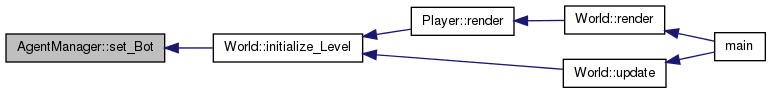
\includegraphics[width=350pt]{class_agent_manager_ab00a9cbf5753546fbb5f9f5cfa1b1241_icgraph}
\end{center}
\end{figure}


\hypertarget{class_agent_manager_a1c05e1578aafde1892a5e4e79862b19f}{\index{Agent\-Manager@{Agent\-Manager}!update@{update}}
\index{update@{update}!AgentManager@{Agent\-Manager}}
\subsubsection[{update}]{\setlength{\rightskip}{0pt plus 5cm}void Agent\-Manager\-::update (
\begin{DoxyParamCaption}
\item[{{\bf Player} $\ast$}]{p\-\_\-\-Temp\-Player, }
\item[{{\bf L\-E\-V\-E\-L\-\_\-\-L\-O\-A\-D\-E\-D}}]{T\-E\-M\-P\-L\-E\-V\-E\-L, }
\item[{S\-D\-L\-\_\-\-Rect}]{camera}
\end{DoxyParamCaption}
)}}\label{class_agent_manager_a1c05e1578aafde1892a5e4e79862b19f}


Hier ist ein Graph, der zeigt, was diese Funktion aufruft\-:\nopagebreak
\begin{figure}[H]
\begin{center}
\leavevmode
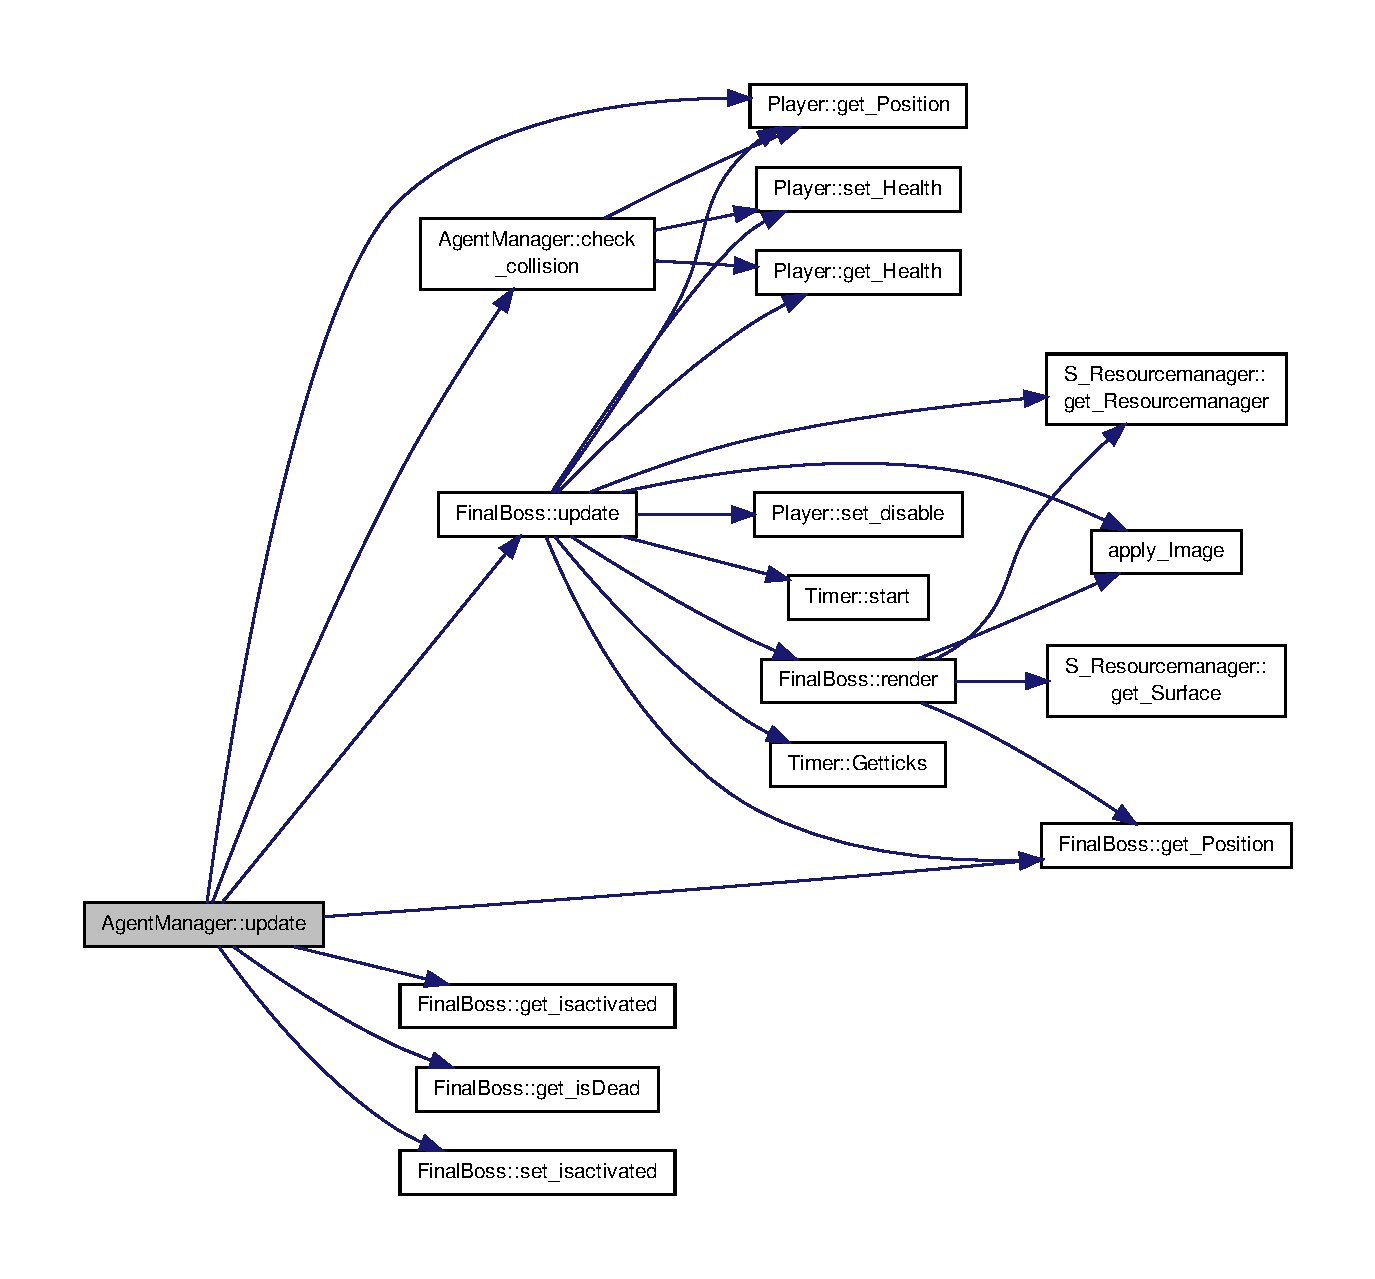
\includegraphics[width=350pt]{class_agent_manager_a1c05e1578aafde1892a5e4e79862b19f_cgraph}
\end{center}
\end{figure}




Hier ist ein Graph der zeigt, wo diese Funktion aufgerufen wird\-:\nopagebreak
\begin{figure}[H]
\begin{center}
\leavevmode
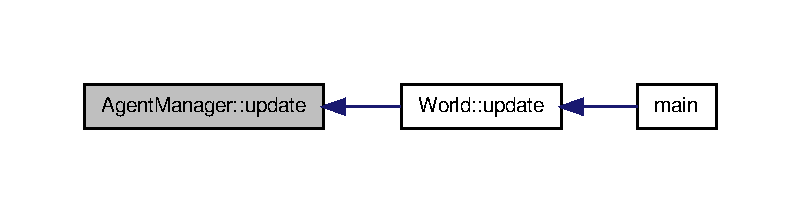
\includegraphics[width=350pt]{class_agent_manager_a1c05e1578aafde1892a5e4e79862b19f_icgraph}
\end{center}
\end{figure}


\hypertarget{class_agent_manager_aafa2ae19bfa65b44dc3c955bd21e0fc3}{\index{Agent\-Manager@{Agent\-Manager}!weaken\-\_\-\-Bots@{weaken\-\_\-\-Bots}}
\index{weaken\-\_\-\-Bots@{weaken\-\_\-\-Bots}!AgentManager@{Agent\-Manager}}
\subsubsection[{weaken\-\_\-\-Bots}]{\setlength{\rightskip}{0pt plus 5cm}void Agent\-Manager\-::weaken\-\_\-\-Bots (
\begin{DoxyParamCaption}
\item[{{\bf Player} $\ast$}]{p\-\_\-\-Temp\-Player}
\end{DoxyParamCaption}
)}}\label{class_agent_manager_aafa2ae19bfa65b44dc3c955bd21e0fc3}


Hier ist ein Graph, der zeigt, was diese Funktion aufruft\-:\nopagebreak
\begin{figure}[H]
\begin{center}
\leavevmode
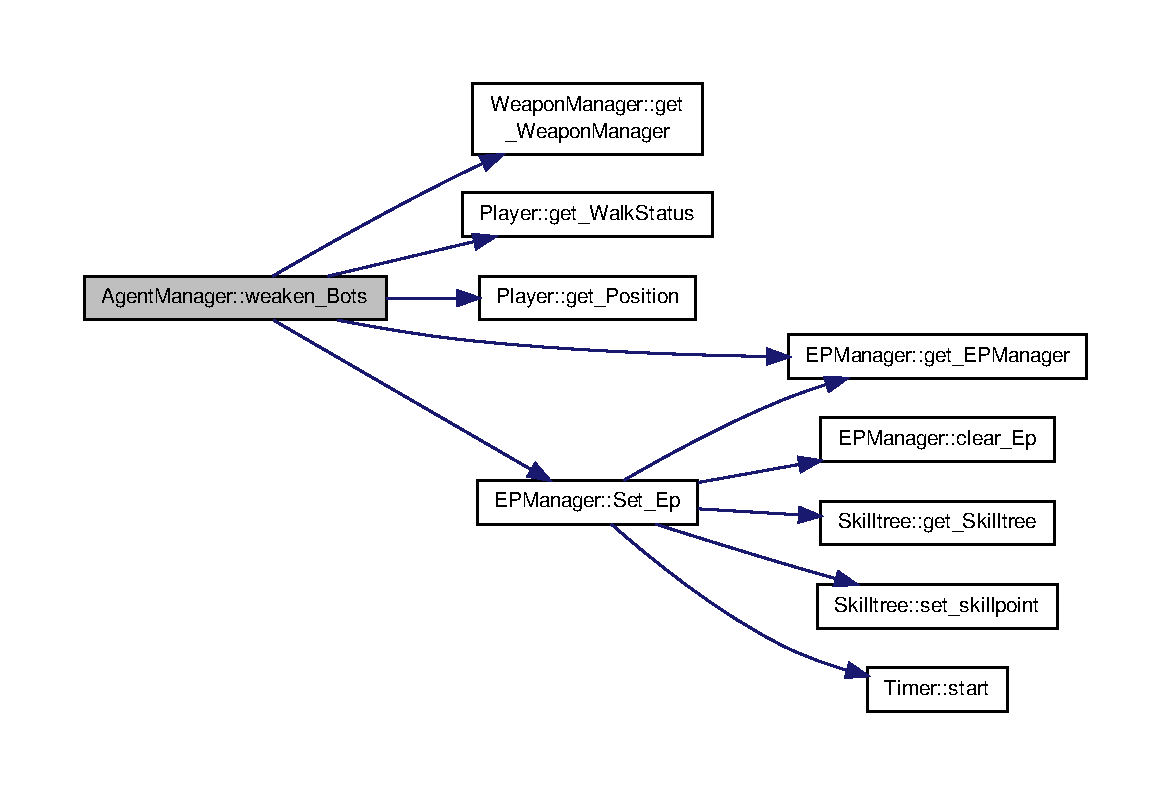
\includegraphics[width=350pt]{class_agent_manager_aafa2ae19bfa65b44dc3c955bd21e0fc3_cgraph}
\end{center}
\end{figure}




Hier ist ein Graph der zeigt, wo diese Funktion aufgerufen wird\-:\nopagebreak
\begin{figure}[H]
\begin{center}
\leavevmode
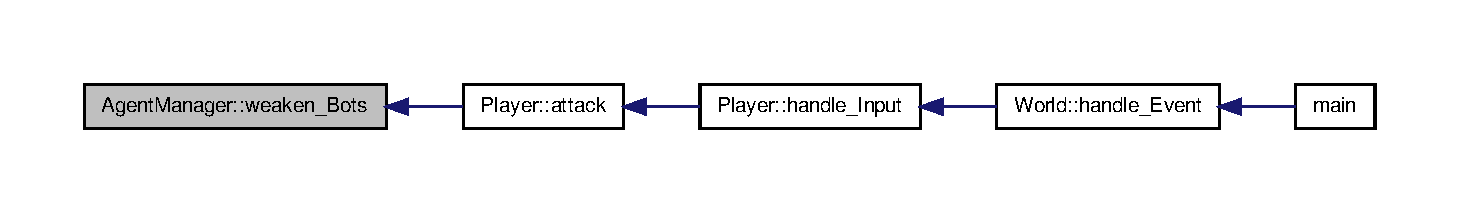
\includegraphics[width=350pt]{class_agent_manager_aafa2ae19bfa65b44dc3c955bd21e0fc3_icgraph}
\end{center}
\end{figure}




\subsection{Dokumentation der Datenelemente}
\hypertarget{class_agent_manager_a1c7aff8c522d35fd1514eb953195be92}{\index{Agent\-Manager@{Agent\-Manager}!all\-Pfleger@{all\-Pfleger}}
\index{all\-Pfleger@{all\-Pfleger}!AgentManager@{Agent\-Manager}}
\subsubsection[{all\-Pfleger}]{\setlength{\rightskip}{0pt plus 5cm}vector$<${\bf Pfleger}$\ast$$>$ Agent\-Manager\-::all\-Pfleger\hspace{0.3cm}{\ttfamily [private]}}}\label{class_agent_manager_a1c7aff8c522d35fd1514eb953195be92}
\hypertarget{class_agent_manager_a3a921dcdcad9845bb40ec0cf67b6cd2e}{\index{Agent\-Manager@{Agent\-Manager}!crazy\-\_\-enemies@{crazy\-\_\-enemies}}
\index{crazy\-\_\-enemies@{crazy\-\_\-enemies}!AgentManager@{Agent\-Manager}}
\subsubsection[{crazy\-\_\-enemies}]{\setlength{\rightskip}{0pt plus 5cm}vector$<${\bf Crazy\-\_\-enemy}$\ast$$>$ Agent\-Manager\-::crazy\-\_\-enemies\hspace{0.3cm}{\ttfamily [private]}}}\label{class_agent_manager_a3a921dcdcad9845bb40ec0cf67b6cd2e}


Vektor der alle Crazy enemies speichert. 

\hypertarget{class_agent_manager_ad04668952fb54954caf87f088eedf4ca}{\index{Agent\-Manager@{Agent\-Manager}!crazy\-\_\-enemies\-To\-Delete@{crazy\-\_\-enemies\-To\-Delete}}
\index{crazy\-\_\-enemies\-To\-Delete@{crazy\-\_\-enemies\-To\-Delete}!AgentManager@{Agent\-Manager}}
\subsubsection[{crazy\-\_\-enemies\-To\-Delete}]{\setlength{\rightskip}{0pt plus 5cm}vector$<${\bf Crazy\-\_\-enemy}$\ast$$>$ Agent\-Manager\-::crazy\-\_\-enemies\-To\-Delete\hspace{0.3cm}{\ttfamily [private]}}}\label{class_agent_manager_ad04668952fb54954caf87f088eedf4ca}
\hypertarget{class_agent_manager_a44183c7f9aa95bfdfab8e2c075d530a3}{\index{Agent\-Manager@{Agent\-Manager}!p\-\_\-\-Boss\-Manager@{p\-\_\-\-Boss\-Manager}}
\index{p\-\_\-\-Boss\-Manager@{p\-\_\-\-Boss\-Manager}!AgentManager@{Agent\-Manager}}
\subsubsection[{p\-\_\-\-Boss\-Manager}]{\setlength{\rightskip}{0pt plus 5cm}{\bf Final\-Boss}$\ast$ Agent\-Manager\-::p\-\_\-\-Boss\-Manager\hspace{0.3cm}{\ttfamily [private]}}}\label{class_agent_manager_a44183c7f9aa95bfdfab8e2c075d530a3}


Die Dokumentation für diese Klasse wurde erzeugt aufgrund der Dateien\-:\begin{DoxyCompactItemize}
\item 
\hyperlink{_agent_manager_8h}{Agent\-Manager.\-h}\item 
\hyperlink{_agentmanager_8cpp}{Agentmanager.\-cpp}\end{DoxyCompactItemize}

\hypertarget{class_armor}{\section{Armor Klassenreferenz}
\label{class_armor}\index{Armor@{Armor}}
}


{\ttfamily \#include $<$Armor.\-h$>$}



Zusammengehörigkeiten von Armor\-:
\nopagebreak
\begin{figure}[H]
\begin{center}
\leavevmode
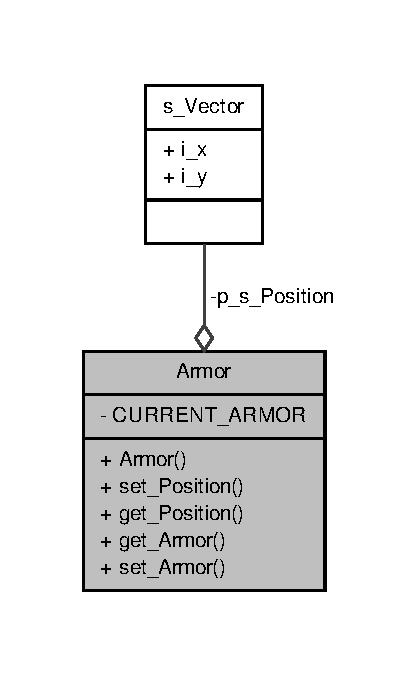
\includegraphics[width=201pt]{class_armor__coll__graph}
\end{center}
\end{figure}
\subsection*{Öffentliche Methoden}
\begin{DoxyCompactItemize}
\item 
\hyperlink{class_armor_ab9f3edb9b0fe736b82056fbfd6abe467}{Armor} (int x, int y, \hyperlink{globals_8h_a8e5f74edbc14259a161d93bd9a69d236}{A\-R\-M\-O\-R\-\_\-\-T\-Y\-P\-E} A\-R\-M\-O\-R\-T\-O\-S\-E\-T)
\item 
void \hyperlink{class_armor_a007fd5929f7cd4c3ab062094c2465371}{set\-\_\-\-Position} (int x, int y)
\item 
\hyperlink{structs___vector}{s\-\_\-\-Vector} $\ast$ \hyperlink{class_armor_aafd49a78e1d9de2ec03bdef3c5b7f454}{get\-\_\-\-Position} ()
\begin{DoxyCompactList}\small\item\em Setzt Ruestungsposition. \end{DoxyCompactList}\item 
\hyperlink{globals_8h_a8e5f74edbc14259a161d93bd9a69d236}{A\-R\-M\-O\-R\-\_\-\-T\-Y\-P\-E} \hyperlink{class_armor_a77760241405973937918be3377b2a02d}{get\-\_\-\-Armor} ()
\item 
void \hyperlink{class_armor_a8c1238b98e8bc91fb39e0e7ef8a331bf}{set\-\_\-\-Armor} (\hyperlink{globals_8h_a8e5f74edbc14259a161d93bd9a69d236}{A\-R\-M\-O\-R\-\_\-\-T\-Y\-P\-E} T\-E\-M\-P\-A\-R\-M\-O\-R)
\begin{DoxyCompactList}\small\item\em Gibt aktuellen Ruestungstyp wieder. \end{DoxyCompactList}\end{DoxyCompactItemize}
\subsection*{Private Attribute}
\begin{DoxyCompactItemize}
\item 
\hyperlink{globals_8h_a8e5f74edbc14259a161d93bd9a69d236}{A\-R\-M\-O\-R\-\_\-\-T\-Y\-P\-E} \hyperlink{class_armor_a41b1d44de440d9bbbcd4c4b8f7757f53}{C\-U\-R\-R\-E\-N\-T\-\_\-\-A\-R\-M\-O\-R}
\item 
\hyperlink{structs___vector}{s\-\_\-\-Vector} $\ast$ \hyperlink{class_armor_a176b9bdfec3dcc70738547f7b8659912}{p\-\_\-s\-\_\-\-Position}
\end{DoxyCompactItemize}


\subsection{Beschreibung der Konstruktoren und Destruktoren}
\hypertarget{class_armor_ab9f3edb9b0fe736b82056fbfd6abe467}{\index{Armor@{Armor}!Armor@{Armor}}
\index{Armor@{Armor}!Armor@{Armor}}
\subsubsection[{Armor}]{\setlength{\rightskip}{0pt plus 5cm}Armor\-::\-Armor (
\begin{DoxyParamCaption}
\item[{int}]{x, }
\item[{int}]{y, }
\item[{{\bf A\-R\-M\-O\-R\-\_\-\-T\-Y\-P\-E}}]{A\-R\-M\-O\-R\-T\-O\-S\-E\-T}
\end{DoxyParamCaption}
)\hspace{0.3cm}{\ttfamily [inline]}}}\label{class_armor_ab9f3edb9b0fe736b82056fbfd6abe467}


\subsection{Dokumentation der Elementfunktionen}
\hypertarget{class_armor_a77760241405973937918be3377b2a02d}{\index{Armor@{Armor}!get\-\_\-\-Armor@{get\-\_\-\-Armor}}
\index{get\-\_\-\-Armor@{get\-\_\-\-Armor}!Armor@{Armor}}
\subsubsection[{get\-\_\-\-Armor}]{\setlength{\rightskip}{0pt plus 5cm}{\bf A\-R\-M\-O\-R\-\_\-\-T\-Y\-P\-E} Armor\-::get\-\_\-\-Armor (
\begin{DoxyParamCaption}
{}
\end{DoxyParamCaption}
)\hspace{0.3cm}{\ttfamily [inline]}}}\label{class_armor_a77760241405973937918be3377b2a02d}
\hypertarget{class_armor_aafd49a78e1d9de2ec03bdef3c5b7f454}{\index{Armor@{Armor}!get\-\_\-\-Position@{get\-\_\-\-Position}}
\index{get\-\_\-\-Position@{get\-\_\-\-Position}!Armor@{Armor}}
\subsubsection[{get\-\_\-\-Position}]{\setlength{\rightskip}{0pt plus 5cm}{\bf s\-\_\-\-Vector}$\ast$ Armor\-::get\-\_\-\-Position (
\begin{DoxyParamCaption}
{}
\end{DoxyParamCaption}
)\hspace{0.3cm}{\ttfamily [inline]}}}\label{class_armor_aafd49a78e1d9de2ec03bdef3c5b7f454}


Setzt Ruestungsposition. 

\hypertarget{class_armor_a8c1238b98e8bc91fb39e0e7ef8a331bf}{\index{Armor@{Armor}!set\-\_\-\-Armor@{set\-\_\-\-Armor}}
\index{set\-\_\-\-Armor@{set\-\_\-\-Armor}!Armor@{Armor}}
\subsubsection[{set\-\_\-\-Armor}]{\setlength{\rightskip}{0pt plus 5cm}void Armor\-::set\-\_\-\-Armor (
\begin{DoxyParamCaption}
\item[{{\bf A\-R\-M\-O\-R\-\_\-\-T\-Y\-P\-E}}]{T\-E\-M\-P\-A\-R\-M\-O\-R}
\end{DoxyParamCaption}
)\hspace{0.3cm}{\ttfamily [inline]}}}\label{class_armor_a8c1238b98e8bc91fb39e0e7ef8a331bf}


Gibt aktuellen Ruestungstyp wieder. 

\hypertarget{class_armor_a007fd5929f7cd4c3ab062094c2465371}{\index{Armor@{Armor}!set\-\_\-\-Position@{set\-\_\-\-Position}}
\index{set\-\_\-\-Position@{set\-\_\-\-Position}!Armor@{Armor}}
\subsubsection[{set\-\_\-\-Position}]{\setlength{\rightskip}{0pt plus 5cm}void Armor\-::set\-\_\-\-Position (
\begin{DoxyParamCaption}
\item[{int}]{x, }
\item[{int}]{y}
\end{DoxyParamCaption}
)\hspace{0.3cm}{\ttfamily [inline]}}}\label{class_armor_a007fd5929f7cd4c3ab062094c2465371}


\subsection{Dokumentation der Datenelemente}
\hypertarget{class_armor_a41b1d44de440d9bbbcd4c4b8f7757f53}{\index{Armor@{Armor}!C\-U\-R\-R\-E\-N\-T\-\_\-\-A\-R\-M\-O\-R@{C\-U\-R\-R\-E\-N\-T\-\_\-\-A\-R\-M\-O\-R}}
\index{C\-U\-R\-R\-E\-N\-T\-\_\-\-A\-R\-M\-O\-R@{C\-U\-R\-R\-E\-N\-T\-\_\-\-A\-R\-M\-O\-R}!Armor@{Armor}}
\subsubsection[{C\-U\-R\-R\-E\-N\-T\-\_\-\-A\-R\-M\-O\-R}]{\setlength{\rightskip}{0pt plus 5cm}{\bf A\-R\-M\-O\-R\-\_\-\-T\-Y\-P\-E} Armor\-::\-C\-U\-R\-R\-E\-N\-T\-\_\-\-A\-R\-M\-O\-R\hspace{0.3cm}{\ttfamily [private]}}}\label{class_armor_a41b1d44de440d9bbbcd4c4b8f7757f53}
\hypertarget{class_armor_a176b9bdfec3dcc70738547f7b8659912}{\index{Armor@{Armor}!p\-\_\-s\-\_\-\-Position@{p\-\_\-s\-\_\-\-Position}}
\index{p\-\_\-s\-\_\-\-Position@{p\-\_\-s\-\_\-\-Position}!Armor@{Armor}}
\subsubsection[{p\-\_\-s\-\_\-\-Position}]{\setlength{\rightskip}{0pt plus 5cm}{\bf s\-\_\-\-Vector}$\ast$ Armor\-::p\-\_\-s\-\_\-\-Position\hspace{0.3cm}{\ttfamily [private]}}}\label{class_armor_a176b9bdfec3dcc70738547f7b8659912}


Die Dokumentation für diese Klasse wurde erzeugt aufgrund der Datei\-:\begin{DoxyCompactItemize}
\item 
\hyperlink{_armor_8h}{Armor.\-h}\end{DoxyCompactItemize}

\hypertarget{class_armor_manager}{\section{Armor\-Manager Klassenreferenz}
\label{class_armor_manager}\index{Armor\-Manager@{Armor\-Manager}}
}
\subsection*{Öffentliche Methoden}
\begin{DoxyCompactItemize}
\item 
\hypertarget{class_armor_manager_ac5fa1487799e07ac40cdc4f44282c65e}{bool {\bfseries find} (A\-R\-M\-O\-R\-\_\-\-T\-Y\-P\-E C\-U\-R\-R\-E\-N\-T\-\_\-\-A\-R\-M\-O\-R)}\label{class_armor_manager_ac5fa1487799e07ac40cdc4f44282c65e}

\item 
\hypertarget{class_armor_manager_a79a20356f9630c6c51a816f0163b28bf}{void {\bfseries render} (S\-D\-L\-\_\-\-Rect camera)}\label{class_armor_manager_a79a20356f9630c6c51a816f0163b28bf}

\item 
\hypertarget{class_armor_manager_a6f608963c4a1efb31b2d658ee5246459}{void {\bfseries update} (\hyperlink{structs___vector}{s\-\_\-\-Vector} $\ast$p\-\_\-\-Position)}\label{class_armor_manager_a6f608963c4a1efb31b2d658ee5246459}

\item 
\hypertarget{class_armor_manager_a4ce4fd2a1570a917b844c740d3164325}{void {\bfseries kill\-\_\-armor} (A\-R\-M\-O\-R\-\_\-\-T\-Y\-P\-E C\-U\-R\-R\-E\-N\-T\-\_\-\-A\-R\-M\-O\-R)}\label{class_armor_manager_a4ce4fd2a1570a917b844c740d3164325}

\item 
\hypertarget{class_armor_manager_a9ee86635d7c7087cc59cb76cbc954d80}{void {\bfseries reinitialize} ()}\label{class_armor_manager_a9ee86635d7c7087cc59cb76cbc954d80}

\item 
\hypertarget{class_armor_manager_a67c0b4d0206bb0916dc2c6f8ca0ee225}{void {\bfseries show} ()}\label{class_armor_manager_a67c0b4d0206bb0916dc2c6f8ca0ee225}

\item 
\hypertarget{class_armor_manager_ae1d12bdafa1ec883841aa311307a3b85}{void {\bfseries set\-\_\-\-Armor} (A\-R\-M\-O\-R\-\_\-\-T\-Y\-P\-E T\-E\-M\-P\-A\-R\-M\-O\-R, int x, int y)}\label{class_armor_manager_ae1d12bdafa1ec883841aa311307a3b85}

\item 
\hypertarget{class_armor_manager_a08b4b1f42b418b09b6917767a3baae74}{A\-R\-M\-O\-R\-\_\-\-T\-Y\-P\-E {\bfseries get\-\_\-\-Armor} ()}\label{class_armor_manager_a08b4b1f42b418b09b6917767a3baae74}

\end{DoxyCompactItemize}
\subsection*{Öffentliche, statische Methoden}
\begin{DoxyCompactItemize}
\item 
\hypertarget{class_armor_manager_ac2d0437101488564e279661ae9078d5a}{static \hyperlink{class_armor_manager}{Armor\-Manager} \& {\bfseries get\-\_\-\-Armor\-Manager} ()}\label{class_armor_manager_ac2d0437101488564e279661ae9078d5a}

\end{DoxyCompactItemize}


Die Dokumentation für diese Klasse wurde erzeugt aufgrund der Dateien\-:\begin{DoxyCompactItemize}
\item 
Armor\-Manager.\-h\item 
Armor\-Manager.\-cpp\end{DoxyCompactItemize}

\hypertarget{class_crazy__enemy}{\section{Crazy\-\_\-enemy Klassenreferenz}
\label{class_crazy__enemy}\index{Crazy\-\_\-enemy@{Crazy\-\_\-enemy}}
}


{\ttfamily \#include $<$Verrückter.\-h$>$}



Klassendiagramm für Crazy\-\_\-enemy\-:
\nopagebreak
\begin{figure}[H]
\begin{center}
\leavevmode
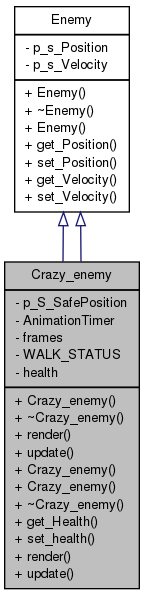
\includegraphics[width=178pt]{class_crazy__enemy__inherit__graph}
\end{center}
\end{figure}


Zusammengehörigkeiten von Crazy\-\_\-enemy\-:
\nopagebreak
\begin{figure}[H]
\begin{center}
\leavevmode
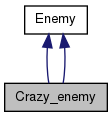
\includegraphics[width=178pt]{class_crazy__enemy__coll__graph}
\end{center}
\end{figure}
\subsection*{Öffentliche Methoden}
\begin{DoxyCompactItemize}
\item 
\hyperlink{class_crazy__enemy_a6043a9ef2ac21fe19481106fc5d32193}{Crazy\-\_\-enemy} ()
\item 
\hyperlink{class_crazy__enemy_aa84f687b9a375a3450c02609f5ea00e2}{$\sim$\-Crazy\-\_\-enemy} ()
\item 
void \hyperlink{class_crazy__enemy_ab3f0fd1c099d35b9a10aaa51064030cc}{render} ()
\item 
void \hyperlink{class_crazy__enemy_adf3b3ef132ca7c300a223af3b4fb4fc7}{update} ()
\item 
\hyperlink{class_crazy__enemy_a6043a9ef2ac21fe19481106fc5d32193}{Crazy\-\_\-enemy} ()
\item 
\hyperlink{class_crazy__enemy_a190c30bf8cc3c818698b3fab6273305a}{Crazy\-\_\-enemy} (int x, int y)
\item 
\hyperlink{class_crazy__enemy_aa84f687b9a375a3450c02609f5ea00e2}{$\sim$\-Crazy\-\_\-enemy} ()
\item 
int \hyperlink{class_crazy__enemy_a475f5dd8aff8e7ed7a0a6c107e510f10}{get\-\_\-\-Health} ()
\begin{DoxyCompactList}\small\item\em Fragt Gesundheit ab. \end{DoxyCompactList}\item 
void \hyperlink{class_crazy__enemy_aca0e6e11b0cf95954141771b710e78ae}{set\-\_\-health} (int t)
\begin{DoxyCompactList}\small\item\em Setzt die Gesundheit. \end{DoxyCompactList}\item 
void \hyperlink{class_crazy__enemy_a4fc63fd437c01b6522beaf468c218f4a}{render} (S\-D\-L\-\_\-\-Rect camera)
\begin{DoxyCompactList}\small\item\em Siehe Verr�ckter.\-cpp. \end{DoxyCompactList}\item 
void \hyperlink{class_crazy__enemy_adf3b3ef132ca7c300a223af3b4fb4fc7}{update} ()
\begin{DoxyCompactList}\small\item\em Siehe Verr�ckter.\-cpp. \end{DoxyCompactList}\end{DoxyCompactItemize}


\subsection{Beschreibung der Konstruktoren und Destruktoren}
\hypertarget{class_crazy__enemy_a6043a9ef2ac21fe19481106fc5d32193}{\index{Crazy\-\_\-enemy@{Crazy\-\_\-enemy}!Crazy\-\_\-enemy@{Crazy\-\_\-enemy}}
\index{Crazy\-\_\-enemy@{Crazy\-\_\-enemy}!Crazy_enemy@{Crazy\-\_\-enemy}}
\subsubsection[{Crazy\-\_\-enemy}]{\setlength{\rightskip}{0pt plus 5cm}Crazy\-\_\-enemy\-::\-Crazy\-\_\-enemy (
\begin{DoxyParamCaption}
{}
\end{DoxyParamCaption}
)\hspace{0.3cm}{\ttfamily [inline]}}}\label{class_crazy__enemy_a6043a9ef2ac21fe19481106fc5d32193}
\hypertarget{class_crazy__enemy_aa84f687b9a375a3450c02609f5ea00e2}{\index{Crazy\-\_\-enemy@{Crazy\-\_\-enemy}!$\sim$\-Crazy\-\_\-enemy@{$\sim$\-Crazy\-\_\-enemy}}
\index{$\sim$\-Crazy\-\_\-enemy@{$\sim$\-Crazy\-\_\-enemy}!Crazy_enemy@{Crazy\-\_\-enemy}}
\subsubsection[{$\sim$\-Crazy\-\_\-enemy}]{\setlength{\rightskip}{0pt plus 5cm}Crazy\-\_\-enemy\-::$\sim$\-Crazy\-\_\-enemy (
\begin{DoxyParamCaption}
{}
\end{DoxyParamCaption}
)\hspace{0.3cm}{\ttfamily [inline]}}}\label{class_crazy__enemy_aa84f687b9a375a3450c02609f5ea00e2}
\hypertarget{class_crazy__enemy_a6043a9ef2ac21fe19481106fc5d32193}{\index{Crazy\-\_\-enemy@{Crazy\-\_\-enemy}!Crazy\-\_\-enemy@{Crazy\-\_\-enemy}}
\index{Crazy\-\_\-enemy@{Crazy\-\_\-enemy}!Crazy_enemy@{Crazy\-\_\-enemy}}
\subsubsection[{Crazy\-\_\-enemy}]{\setlength{\rightskip}{0pt plus 5cm}Crazy\-\_\-enemy\-::\-Crazy\-\_\-enemy (
\begin{DoxyParamCaption}
{}
\end{DoxyParamCaption}
)\hspace{0.3cm}{\ttfamily [inline]}}}\label{class_crazy__enemy_a6043a9ef2ac21fe19481106fc5d32193}
\hypertarget{class_crazy__enemy_a190c30bf8cc3c818698b3fab6273305a}{\index{Crazy\-\_\-enemy@{Crazy\-\_\-enemy}!Crazy\-\_\-enemy@{Crazy\-\_\-enemy}}
\index{Crazy\-\_\-enemy@{Crazy\-\_\-enemy}!Crazy_enemy@{Crazy\-\_\-enemy}}
\subsubsection[{Crazy\-\_\-enemy}]{\setlength{\rightskip}{0pt plus 5cm}Crazy\-\_\-enemy\-::\-Crazy\-\_\-enemy (
\begin{DoxyParamCaption}
\item[{int}]{x, }
\item[{int}]{y}
\end{DoxyParamCaption}
)\hspace{0.3cm}{\ttfamily [inline]}}}\label{class_crazy__enemy_a190c30bf8cc3c818698b3fab6273305a}


Hier ist ein Graph, der zeigt, was diese Funktion aufruft\-:
\nopagebreak
\begin{figure}[H]
\begin{center}
\leavevmode
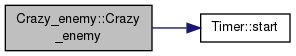
\includegraphics[width=294pt]{class_crazy__enemy_a190c30bf8cc3c818698b3fab6273305a_cgraph}
\end{center}
\end{figure}


\hypertarget{class_crazy__enemy_aa84f687b9a375a3450c02609f5ea00e2}{\index{Crazy\-\_\-enemy@{Crazy\-\_\-enemy}!$\sim$\-Crazy\-\_\-enemy@{$\sim$\-Crazy\-\_\-enemy}}
\index{$\sim$\-Crazy\-\_\-enemy@{$\sim$\-Crazy\-\_\-enemy}!Crazy_enemy@{Crazy\-\_\-enemy}}
\subsubsection[{$\sim$\-Crazy\-\_\-enemy}]{\setlength{\rightskip}{0pt plus 5cm}Crazy\-\_\-enemy\-::$\sim$\-Crazy\-\_\-enemy (
\begin{DoxyParamCaption}
{}
\end{DoxyParamCaption}
)\hspace{0.3cm}{\ttfamily [inline]}}}\label{class_crazy__enemy_aa84f687b9a375a3450c02609f5ea00e2}


\subsection{Dokumentation der Elementfunktionen}
\hypertarget{class_crazy__enemy_a475f5dd8aff8e7ed7a0a6c107e510f10}{\index{Crazy\-\_\-enemy@{Crazy\-\_\-enemy}!get\-\_\-\-Health@{get\-\_\-\-Health}}
\index{get\-\_\-\-Health@{get\-\_\-\-Health}!Crazy_enemy@{Crazy\-\_\-enemy}}
\subsubsection[{get\-\_\-\-Health}]{\setlength{\rightskip}{0pt plus 5cm}int Crazy\-\_\-enemy\-::get\-\_\-\-Health (
\begin{DoxyParamCaption}
{}
\end{DoxyParamCaption}
)\hspace{0.3cm}{\ttfamily [inline]}}}\label{class_crazy__enemy_a475f5dd8aff8e7ed7a0a6c107e510f10}


Fragt Gesundheit ab. 

\hypertarget{class_crazy__enemy_ab3f0fd1c099d35b9a10aaa51064030cc}{\index{Crazy\-\_\-enemy@{Crazy\-\_\-enemy}!render@{render}}
\index{render@{render}!Crazy_enemy@{Crazy\-\_\-enemy}}
\subsubsection[{render}]{\setlength{\rightskip}{0pt plus 5cm}void Crazy\-\_\-enemy\-::render (
\begin{DoxyParamCaption}
{}
\end{DoxyParamCaption}
)}}\label{class_crazy__enemy_ab3f0fd1c099d35b9a10aaa51064030cc}


Hier ist ein Graph, der zeigt, was diese Funktion aufruft\-:
\nopagebreak
\begin{figure}[H]
\begin{center}
\leavevmode
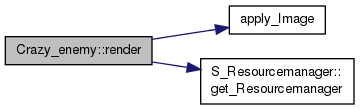
\includegraphics[width=342pt]{class_crazy__enemy_ab3f0fd1c099d35b9a10aaa51064030cc_cgraph}
\end{center}
\end{figure}


\hypertarget{class_crazy__enemy_a4fc63fd437c01b6522beaf468c218f4a}{\index{Crazy\-\_\-enemy@{Crazy\-\_\-enemy}!render@{render}}
\index{render@{render}!Crazy_enemy@{Crazy\-\_\-enemy}}
\subsubsection[{render}]{\setlength{\rightskip}{0pt plus 5cm}void Crazy\-\_\-enemy\-::render (
\begin{DoxyParamCaption}
\item[{S\-D\-L\-\_\-\-Rect}]{camera}
\end{DoxyParamCaption}
)}}\label{class_crazy__enemy_a4fc63fd437c01b6522beaf468c218f4a}


Siehe Verr�ckter.\-cpp. 

Rendert den Verrueckten. 

Hier ist ein Graph, der zeigt, was diese Funktion aufruft\-:
\nopagebreak
\begin{figure}[H]
\begin{center}
\leavevmode
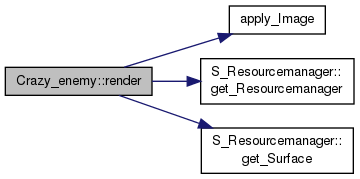
\includegraphics[width=342pt]{class_crazy__enemy_a4fc63fd437c01b6522beaf468c218f4a_cgraph}
\end{center}
\end{figure}


\hypertarget{class_crazy__enemy_aca0e6e11b0cf95954141771b710e78ae}{\index{Crazy\-\_\-enemy@{Crazy\-\_\-enemy}!set\-\_\-health@{set\-\_\-health}}
\index{set\-\_\-health@{set\-\_\-health}!Crazy_enemy@{Crazy\-\_\-enemy}}
\subsubsection[{set\-\_\-health}]{\setlength{\rightskip}{0pt plus 5cm}void Crazy\-\_\-enemy\-::set\-\_\-health (
\begin{DoxyParamCaption}
\item[{int}]{t}
\end{DoxyParamCaption}
)\hspace{0.3cm}{\ttfamily [inline]}}}\label{class_crazy__enemy_aca0e6e11b0cf95954141771b710e78ae}


Setzt die Gesundheit. 

\hypertarget{class_crazy__enemy_adf3b3ef132ca7c300a223af3b4fb4fc7}{\index{Crazy\-\_\-enemy@{Crazy\-\_\-enemy}!update@{update}}
\index{update@{update}!Crazy_enemy@{Crazy\-\_\-enemy}}
\subsubsection[{update}]{\setlength{\rightskip}{0pt plus 5cm}void Crazy\-\_\-enemy\-::update (
\begin{DoxyParamCaption}
{}
\end{DoxyParamCaption}
)}}\label{class_crazy__enemy_adf3b3ef132ca7c300a223af3b4fb4fc7}
Verwaltet die Bewegung des Verrueckten \hypertarget{class_crazy__enemy_adf3b3ef132ca7c300a223af3b4fb4fc7}{\index{Crazy\-\_\-enemy@{Crazy\-\_\-enemy}!update@{update}}
\index{update@{update}!Crazy_enemy@{Crazy\-\_\-enemy}}
\subsubsection[{update}]{\setlength{\rightskip}{0pt plus 5cm}void Crazy\-\_\-enemy\-::update (
\begin{DoxyParamCaption}
{}
\end{DoxyParamCaption}
)}}\label{class_crazy__enemy_adf3b3ef132ca7c300a223af3b4fb4fc7}


Siehe Verr�ckter.\-cpp. 



Die Dokumentation für diese Klasse wurde erzeugt aufgrund der Dateien\-:\begin{DoxyCompactItemize}
\item 
\hyperlink{_crazy__enemy_8cpp}{Crazy\-\_\-enemy.\-cpp}\item 
\hyperlink{_verr_xC3_xBCckter_8h}{Verrückter.\-h}\item 
\hyperlink{_crazy__enemy_8h}{Crazy\-\_\-enemy.\-h}\item 
\hyperlink{_verr_xC3_xBCckter_8cpp}{Verrückter.\-cpp}\end{DoxyCompactItemize}

\hypertarget{class_endboss}{\section{Endboss Klassenreferenz}
\label{class_endboss}\index{Endboss@{Endboss}}
}


{\ttfamily \#include $<$Endboss.\-h$>$}



Klassendiagramm für Endboss\-:
\nopagebreak
\begin{figure}[H]
\begin{center}
\leavevmode
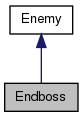
\includegraphics[width=166pt]{class_endboss__inherit__graph}
\end{center}
\end{figure}


Zusammengehörigkeiten von Endboss\-:
\nopagebreak
\begin{figure}[H]
\begin{center}
\leavevmode
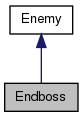
\includegraphics[width=166pt]{class_endboss__coll__graph}
\end{center}
\end{figure}
\subsection*{Öffentliche Methoden}
\begin{DoxyCompactItemize}
\item 
\hyperlink{class_endboss_a07721dbe95bf63097d021b8b2a80791b}{Endboss} ()
\item 
\hyperlink{class_endboss_a6d553673da1e7b3d09ce54cd2503cbb7}{Endboss} (int x, int y)
\item 
\hyperlink{class_endboss_ab86f4e842ac4116c8df943539cc43787}{$\sim$\-Endboss} ()
\item 
int \hyperlink{class_endboss_a69ae2922f0f6647037926e917da4ee5e}{get\-\_\-\-Health} ()
\item 
void \hyperlink{class_endboss_a0bbf59647d911c6380246de92b5f5e21}{set\-\_\-health} (int t)
\item 
void \hyperlink{class_endboss_a17b150268f358172b140a984aaaa61c8}{render} (S\-D\-L\-\_\-\-Rect camera)
\item 
void \hyperlink{class_endboss_a7a56e4b087239ff73b7810c967e3858f}{update} ()
\end{DoxyCompactItemize}


\subsection{Beschreibung der Konstruktoren und Destruktoren}
\hypertarget{class_endboss_a07721dbe95bf63097d021b8b2a80791b}{\index{Endboss@{Endboss}!Endboss@{Endboss}}
\index{Endboss@{Endboss}!Endboss@{Endboss}}
\subsubsection[{Endboss}]{\setlength{\rightskip}{0pt plus 5cm}Endboss\-::\-Endboss (
\begin{DoxyParamCaption}
{}
\end{DoxyParamCaption}
)\hspace{0.3cm}{\ttfamily [inline]}}}\label{class_endboss_a07721dbe95bf63097d021b8b2a80791b}
\hypertarget{class_endboss_a6d553673da1e7b3d09ce54cd2503cbb7}{\index{Endboss@{Endboss}!Endboss@{Endboss}}
\index{Endboss@{Endboss}!Endboss@{Endboss}}
\subsubsection[{Endboss}]{\setlength{\rightskip}{0pt plus 5cm}Endboss\-::\-Endboss (
\begin{DoxyParamCaption}
\item[{int}]{x, }
\item[{int}]{y}
\end{DoxyParamCaption}
)\hspace{0.3cm}{\ttfamily [inline]}}}\label{class_endboss_a6d553673da1e7b3d09ce54cd2503cbb7}


Hier ist ein Graph, der zeigt, was diese Funktion aufruft\-:
\nopagebreak
\begin{figure}[H]
\begin{center}
\leavevmode
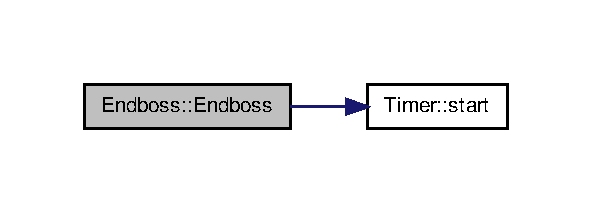
\includegraphics[width=284pt]{class_endboss_a6d553673da1e7b3d09ce54cd2503cbb7_cgraph}
\end{center}
\end{figure}


\hypertarget{class_endboss_ab86f4e842ac4116c8df943539cc43787}{\index{Endboss@{Endboss}!$\sim$\-Endboss@{$\sim$\-Endboss}}
\index{$\sim$\-Endboss@{$\sim$\-Endboss}!Endboss@{Endboss}}
\subsubsection[{$\sim$\-Endboss}]{\setlength{\rightskip}{0pt plus 5cm}Endboss\-::$\sim$\-Endboss (
\begin{DoxyParamCaption}
{}
\end{DoxyParamCaption}
)\hspace{0.3cm}{\ttfamily [inline]}}}\label{class_endboss_ab86f4e842ac4116c8df943539cc43787}


\subsection{Dokumentation der Elementfunktionen}
\hypertarget{class_endboss_a69ae2922f0f6647037926e917da4ee5e}{\index{Endboss@{Endboss}!get\-\_\-\-Health@{get\-\_\-\-Health}}
\index{get\-\_\-\-Health@{get\-\_\-\-Health}!Endboss@{Endboss}}
\subsubsection[{get\-\_\-\-Health}]{\setlength{\rightskip}{0pt plus 5cm}int Endboss\-::get\-\_\-\-Health (
\begin{DoxyParamCaption}
{}
\end{DoxyParamCaption}
)\hspace{0.3cm}{\ttfamily [inline]}}}\label{class_endboss_a69ae2922f0f6647037926e917da4ee5e}
\hypertarget{class_endboss_a17b150268f358172b140a984aaaa61c8}{\index{Endboss@{Endboss}!render@{render}}
\index{render@{render}!Endboss@{Endboss}}
\subsubsection[{render}]{\setlength{\rightskip}{0pt plus 5cm}void Endboss\-::render (
\begin{DoxyParamCaption}
\item[{S\-D\-L\-\_\-\-Rect}]{camera}
\end{DoxyParamCaption}
)}}\label{class_endboss_a17b150268f358172b140a984aaaa61c8}


Hier ist ein Graph, der zeigt, was diese Funktion aufruft\-:
\nopagebreak
\begin{figure}[H]
\begin{center}
\leavevmode
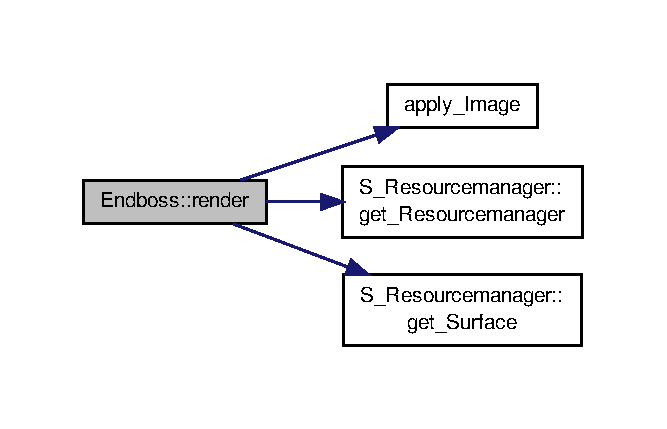
\includegraphics[width=320pt]{class_endboss_a17b150268f358172b140a984aaaa61c8_cgraph}
\end{center}
\end{figure}


\hypertarget{class_endboss_a0bbf59647d911c6380246de92b5f5e21}{\index{Endboss@{Endboss}!set\-\_\-health@{set\-\_\-health}}
\index{set\-\_\-health@{set\-\_\-health}!Endboss@{Endboss}}
\subsubsection[{set\-\_\-health}]{\setlength{\rightskip}{0pt plus 5cm}void Endboss\-::set\-\_\-health (
\begin{DoxyParamCaption}
\item[{int}]{t}
\end{DoxyParamCaption}
)\hspace{0.3cm}{\ttfamily [inline]}}}\label{class_endboss_a0bbf59647d911c6380246de92b5f5e21}
\hypertarget{class_endboss_a7a56e4b087239ff73b7810c967e3858f}{\index{Endboss@{Endboss}!update@{update}}
\index{update@{update}!Endboss@{Endboss}}
\subsubsection[{update}]{\setlength{\rightskip}{0pt plus 5cm}void Endboss\-::update (
\begin{DoxyParamCaption}
{}
\end{DoxyParamCaption}
)}}\label{class_endboss_a7a56e4b087239ff73b7810c967e3858f}


Die Dokumentation für diese Klasse wurde erzeugt aufgrund der Dateien\-:\begin{DoxyCompactItemize}
\item 
\hyperlink{_endboss_8h}{Endboss.\-h}\item 
\hyperlink{_endboss_8cpp}{Endboss.\-cpp}\end{DoxyCompactItemize}

\hypertarget{class_enemy}{\section{Enemy Klassenreferenz}
\label{class_enemy}\index{Enemy@{Enemy}}
}


Klassendiagramm für Enemy\-:
\subsection*{Öffentliche Methoden}
\begin{DoxyCompactItemize}
\item 
\hypertarget{class_enemy_a98f0d2110309536798101b88d2d1d8c9}{{\bfseries Enemy} (int x, int y)}\label{class_enemy_a98f0d2110309536798101b88d2d1d8c9}

\item 
\hypertarget{class_enemy_a8894742ec191ae32c4e22014e5af8246}{\hyperlink{structs___vector}{s\-\_\-\-Vector} $\ast$ {\bfseries get\-\_\-\-Position} ()}\label{class_enemy_a8894742ec191ae32c4e22014e5af8246}

\item 
\hypertarget{class_enemy_a39b8b0f9a87bf2a7b6ee8a1f59cefcf4}{void {\bfseries set\-\_\-\-Position} (int i\-\_\-x, int i\-\_\-y)}\label{class_enemy_a39b8b0f9a87bf2a7b6ee8a1f59cefcf4}

\item 
\hypertarget{class_enemy_a01024ba4588c4ab2efc9a9e0a960c983}{\hyperlink{structs___vector}{s\-\_\-\-Vector} $\ast$ {\bfseries get\-\_\-\-Velocity} ()}\label{class_enemy_a01024ba4588c4ab2efc9a9e0a960c983}

\item 
\hypertarget{class_enemy_ab026b4302720f1676653285b27babd59}{void {\bfseries set\-\_\-\-Velocity} (int i\-\_\-x, int i\-\_\-y)}\label{class_enemy_ab026b4302720f1676653285b27babd59}

\end{DoxyCompactItemize}


Die Dokumentation für diese Klasse wurde erzeugt aufgrund der Datei\-:\begin{DoxyCompactItemize}
\item 
Enemy.\-h\end{DoxyCompactItemize}

\hypertarget{class_e_p_manager}{\section{E\-P\-Manager Klassenreferenz}
\label{class_e_p_manager}\index{E\-P\-Manager@{E\-P\-Manager}}
}
\subsection*{Öffentliche Methoden}
\begin{DoxyCompactItemize}
\item 
\hypertarget{class_e_p_manager_ab16a464979242e27ab1de48a2fa8d193}{void {\bfseries clear\-\_\-\-Ep} ()}\label{class_e_p_manager_ab16a464979242e27ab1de48a2fa8d193}

\item 
\hypertarget{class_e_p_manager_ae0839a39f9ee6fd51d67faafbd6ff560}{void {\bfseries render} ()}\label{class_e_p_manager_ae0839a39f9ee6fd51d67faafbd6ff560}

\item 
\hypertarget{class_e_p_manager_aadec631b4cc9f5de5f4f8040aeeb1778}{int {\bfseries get\-\_\-\-Ep} ()}\label{class_e_p_manager_aadec631b4cc9f5de5f4f8040aeeb1778}

\item 
\hypertarget{class_e_p_manager_a300554dc6cd44d47ece8ebe6d8ed2daa}{void {\bfseries Set\-\_\-\-Ep} (int specep)}\label{class_e_p_manager_a300554dc6cd44d47ece8ebe6d8ed2daa}

\item 
\hypertarget{class_e_p_manager_af8b59848547dee1ab3967aaebcf8fc3a}{int {\bfseries get\-\_\-level} ()}\label{class_e_p_manager_af8b59848547dee1ab3967aaebcf8fc3a}

\item 
\hypertarget{class_e_p_manager_ad6ec1c64ea6b54f646bb793ad53e0279}{bool {\bfseries level\-\_\-up} ()}\label{class_e_p_manager_ad6ec1c64ea6b54f646bb793ad53e0279}

\item 
\hypertarget{class_e_p_manager_a1eac7449962fd356c97f588dbbf0e39e}{void {\bfseries carry\-\_\-point} ()}\label{class_e_p_manager_a1eac7449962fd356c97f588dbbf0e39e}

\end{DoxyCompactItemize}
\subsection*{Öffentliche, statische Methoden}
\begin{DoxyCompactItemize}
\item 
\hypertarget{class_e_p_manager_a7dd8287b28c4c0fc6e39e8846ee4bbc5}{static \hyperlink{class_e_p_manager}{E\-P\-Manager} \& {\bfseries get\-\_\-\-E\-P\-Manager} ()}\label{class_e_p_manager_a7dd8287b28c4c0fc6e39e8846ee4bbc5}

\end{DoxyCompactItemize}


Die Dokumentation für diese Klasse wurde erzeugt aufgrund der Dateien\-:\begin{DoxyCompactItemize}
\item 
E\-P\-Manager.\-h\item 
E\-P\-Manager.\-cpp\end{DoxyCompactItemize}

\hypertarget{class_final_boss}{\section{Final\-Boss Klassenreferenz}
\label{class_final_boss}\index{Final\-Boss@{Final\-Boss}}
}
\subsection*{Öffentliche Methoden}
\begin{DoxyCompactItemize}
\item 
\hypertarget{class_final_boss_a6c30600b7492a40d2ec99874d41296b0}{\hyperlink{structs___vector}{s\-\_\-\-Vector} $\ast$ {\bfseries get\-\_\-\-Position} ()}\label{class_final_boss_a6c30600b7492a40d2ec99874d41296b0}

\item 
\hypertarget{class_final_boss_a65029b764ec03a87caf71e7687d23306}{void {\bfseries set\-\_\-\-Position} (int i\-\_\-x, int i\-\_\-y)}\label{class_final_boss_a65029b764ec03a87caf71e7687d23306}

\item 
\hypertarget{class_final_boss_abacad04a4ff64dd94b3338b7cab122f2}{bool {\bfseries get\-\_\-is\-Dead} ()}\label{class_final_boss_abacad04a4ff64dd94b3338b7cab122f2}

\item 
\hypertarget{class_final_boss_aa0baaf57ed8bacb2174fbcc65b75cec9}{bool {\bfseries get\-\_\-isactivated} ()}\label{class_final_boss_aa0baaf57ed8bacb2174fbcc65b75cec9}

\item 
\hypertarget{class_final_boss_aa9ee8f4ddea7ecfc2d7b9bbaf6ca73a6}{void {\bfseries set\-\_\-isactivated} (bool t)}\label{class_final_boss_aa9ee8f4ddea7ecfc2d7b9bbaf6ca73a6}

\item 
void \hyperlink{class_final_boss_a0dfe88f2e430bd3a8760801809ab7c01}{render} (S\-D\-L\-\_\-\-Rect camera)
\item 
void \hyperlink{class_final_boss_a201e58c54ae09fbfd97bf6ef4fb2843f}{update} (\hyperlink{class_player}{Player} $\ast$p\-\_\-\-Player, S\-D\-L\-\_\-\-Rect camera)
\item 
\hypertarget{class_final_boss_a1579fd9da81da66bbed75799f7113be9}{void {\bfseries weaken\-\_\-\-Endboss} (\hyperlink{class_player}{Player} $\ast$p\-\_\-\-Temp\-Player)}\label{class_final_boss_a1579fd9da81da66bbed75799f7113be9}

\end{DoxyCompactItemize}


\subsection{Dokumentation der Elementfunktionen}
\hypertarget{class_final_boss_a0dfe88f2e430bd3a8760801809ab7c01}{\index{Final\-Boss@{Final\-Boss}!render@{render}}
\index{render@{render}!FinalBoss@{Final\-Boss}}
\subsubsection[{render}]{\setlength{\rightskip}{0pt plus 5cm}void Final\-Boss\-::render (
\begin{DoxyParamCaption}
\item[{S\-D\-L\-\_\-\-Rect}]{camera}
\end{DoxyParamCaption}
)}}\label{class_final_boss_a0dfe88f2e430bd3a8760801809ab7c01}
apply\-\_\-\-Image(0,0,\hyperlink{class_s___resourcemanager_a785fd4b8631a35647823bd41c28ae2d0}{S\-\_\-\-Resourcemanager\-::get\-\_\-\-Resourcemanager()}-\/$>$get\-\_\-\-Surface(\char`\"{}\-Win\char`\"{}),\hyperlink{class_s___resourcemanager_a785fd4b8631a35647823bd41c28ae2d0}{S\-\_\-\-Resourcemanager\-::get\-\_\-\-Resourcemanager()}-\/$>$get\-\_\-\-Surface(\char`\"{}\-Screen\char`\"{})); S\-D\-L\-\_\-\-Flip(\hyperlink{class_s___resourcemanager_a785fd4b8631a35647823bd41c28ae2d0}{S\-\_\-\-Resourcemanager\-::get\-\_\-\-Resourcemanager()}-\/$>$get\-\_\-\-Surface(\char`\"{}\-Screen\char`\"{})); S\-D\-L\-\_\-\-Delay(5000); tempplayer-\/$>$set\-\_\-\-Health(100); tempplayer-\/$>$set\-\_\-\-Position(0,0); $\ast$tempmenue = true; 

Hier ist ein Graph, der zeigt, was diese Funktion aufruft\-:
\nopagebreak
\begin{figure}[H]
\begin{center}
\leavevmode
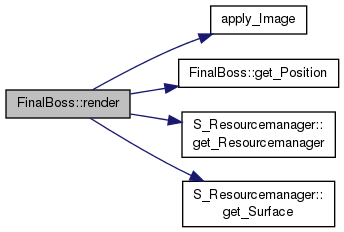
\includegraphics[width=326pt]{class_final_boss_a0dfe88f2e430bd3a8760801809ab7c01_cgraph}
\end{center}
\end{figure}




Hier ist ein Graph der zeigt, wo diese Funktion aufgerufen wird\-:
\nopagebreak
\begin{figure}[H]
\begin{center}
\leavevmode
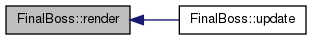
\includegraphics[width=306pt]{class_final_boss_a0dfe88f2e430bd3a8760801809ab7c01_icgraph}
\end{center}
\end{figure}


\hypertarget{class_final_boss_a201e58c54ae09fbfd97bf6ef4fb2843f}{\index{Final\-Boss@{Final\-Boss}!update@{update}}
\index{update@{update}!FinalBoss@{Final\-Boss}}
\subsubsection[{update}]{\setlength{\rightskip}{0pt plus 5cm}void Final\-Boss\-::update (
\begin{DoxyParamCaption}
\item[{{\bf Player} $\ast$}]{p\-\_\-\-Player, }
\item[{S\-D\-L\-\_\-\-Rect}]{camera}
\end{DoxyParamCaption}
)}}\label{class_final_boss_a201e58c54ae09fbfd97bf6ef4fb2843f}
Bewegungsteil\-\_\-\-\_\-\-\_\-\-\_\-\-\_\-\-\_\-\-\_\-\-\_\-\-\_\-\-\_\-\-\_\-\-\_\-\-\_\-\-\_\-\-\_\-\-\_\-\-\_\-\-\_\-\-\_\-\-\_\-\-\_\-\-\_\-\-\_\-\-\_\-\-\_\-\-\_\-\-\_\-\-\_\-\-\_\-\-\_\-\-\_\-\-\_\-\-\_\-\-\_\-\-\_\-\-\_\-\-\_\-\-\_\-\-\_\-\-\_\-\-\_\-\-\_\-\-\_\-\-\_\-\-\_\-\-\_\-\-\_\-\-\_\-\-\_\-\-\_\-\-\_\-\-\_\-\-\_\-\-\_\-\-\_\-\-\_\-\-\_\-\-\_\-\-\_\-\-\_\-\-\_\-\-\_\-\-\_\-\-\_\-\-\_\-\-\_\-\-\_\-\-\_\-\-\_\-\-\_\-\-\_\-\-\_\-\-\_\-\-\_\-\-\_\-\-\_\-\-\_\-\-\_\-\-\_\-\-\_\-\-\_\-\-\_\-\-\_\-\-\_\-\-\_\-\-\_\-\-\_\-\-\_\-\-\_\-\-\_\-\-\_\-\-\_\-\-\_\-\-\_\-\-\_\-\-\_\-\-\_\-\-\_\-\-\_\-\-\_\-\-\_\-\-\_\-\-\_\-\-\_\-\-\_\-\-\_\-\-\_\-\-\_\-\-\_\-\-\_\-\-\_\-\-\_\-\-\_\-\-\_\-\-\_\-\-\_\-\-\_\-\-\_\-\-\_\-\-\_\-\-\_\-\-\_\-\-\_\-\-\_\-\-\_\-\-\_\-\-\_\-\-\_\-\-\_\-

E\-N\-D\-E B\-Ewegungsteil\-\_\-\-\_\-\-\_\-\-\_\-\-\_\-\-\_\-\-\_\-\-\_\-\-\_\-\-\_\-\-\_\-\-\_\-\-\_\-\-\_\-\-\_\-\-\_\-\-\_\-\-\_\-\-\_\-\-\_\-\-\_\-\-\_\-\-\_\-\-\_\-\-\_\-\-\_\-\-\_\-\-\_\-\-\_\-\-\_\-\-\_\-\-\_\-\-\_\-\-\_\-\-\_\-\-\_\-\-\_\-\-\_\-\-\_\-\-\_\-\-\_\-\-\_\-\-\_\-\-\_\-\-\_\-\-\_\-\-\_\-\-\_\-\-\_\-\-\_\-\-\_\-\-\_\-\-\_\-\-\_\-\-\_\-\-\_\-\-\_\-\-\_\-\-\_\-\-\_\-\-\_\-\-\_\-\-\_\-\-\_\-\-\_\-\-\_\-\-\_\-\-\_\-\-\_\-\-\_\-\-\_\-\-\_\-\-\_\-\-\_\-\-\_\-\-\_\-\-\_\-\-\_\-\-\_\-\-\_\-\-\_\-\-\_\-\-\_\-\-\_\-\-\_\-\-\_\-\-\_\-\-\_\-\-\_\-\-\_\-\-\_\-\-\_\-\-\_\-\-\_\-\-\_\-\-\_\-\-\_\-\-\_\-\-\_\-\-\_\-\-\_\-\-\_\-\-\_\-\-\_\-\-\_\-\-\_\-\-\_\-\-\_\-\-\_\-\-\_\-\-\_\-\-\_\-\-\_\-

Anfang Schadenssetzungsteil\-\_\-\-\_\-\-\_\-\-\_\-\-\_\-\-\_\-\-\_\-\-\_\-\-\_\-\-\_\-\-\_\-\-\_\-\-\_\-\-\_\-\-\_\-\-\_\-\-\_\-\-\_\-\-\_\-\-\_\-\-\_\-\-\_\-\-\_\-\-\_\-\-\_\-\-\_\-\-\_\-\-\_\-\-\_\-\-\_\-\-\_\-\-\_\-\-\_\-\-\_\-\-\_\-\-\_\-\-\_\-\-\_\-\-\_\-\-\_\-\-\_\-\-\_\-\-\_\-\-\_\-\-\_\-\-\_\-\-\_\-\-\_\-\-\_\-\-\_\-\-\_\-\-\_\-\-\_\-\-\_\-\-\_\-\-\_\-\-\_\-\-\_\-\-\_\-\-\_\-\-\_\-\-\_\-\-\_\-\-\_\-\-\_\-\-\_\-\-\_\-\-\_\-\-\_\-\-\_\-\-\_\-\-\_\-\-\_\-\-\_\-\-\_\-\-\_\-\-\_\-\-\_\-\-\_\-\-\_\-\-\_\-\-\_\-\-\_\-\-\_\-\-\_\-\-\_\-\-\_\-\-\_\-\-\_\-\-\_\-\-\_\-\-\_\-\-\_\-\-\_\-\-\_\-\-\_\-\-\_\-\-\_\-\-\_\-\-\_\-\-\_\-\-\_\-\-\_\-\-\_\-\-\_\-\-\_\- 

Hier ist ein Graph, der zeigt, was diese Funktion aufruft\-:
\nopagebreak
\begin{figure}[H]
\begin{center}
\leavevmode
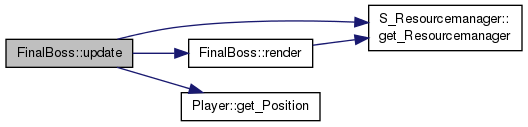
\includegraphics[width=350pt]{class_final_boss_a201e58c54ae09fbfd97bf6ef4fb2843f_cgraph}
\end{center}
\end{figure}




Die Dokumentation für diese Klasse wurde erzeugt aufgrund der Dateien\-:\begin{DoxyCompactItemize}
\item 
Final\-Boss.\-h\item 
Final\-Boss.\-cpp\end{DoxyCompactItemize}

\hypertarget{class_item}{\section{Item Klassenreferenz}
\label{class_item}\index{Item@{Item}}
}
\subsection*{Öffentliche Methoden}
\begin{DoxyCompactItemize}
\item 
\hypertarget{class_item_ae203ad5350de1aa73defd90973e055f0}{{\bfseries Item} (int x, int y, I\-T\-E\-M\-\_\-\-T\-Y\-P\-E I\-T\-E\-M\-T\-O\-S\-E\-T)}\label{class_item_ae203ad5350de1aa73defd90973e055f0}

\item 
\hypertarget{class_item_afcee83c2911215a53019b9182a37eb9f}{I\-T\-E\-M\-\_\-\-T\-Y\-P\-E {\bfseries get\-\_\-\-Item} ()}\label{class_item_afcee83c2911215a53019b9182a37eb9f}

\item 
\hypertarget{class_item_a00a562954be3b3ce018676aea84d9a75}{void {\bfseries set\-\_\-\-Item} (I\-T\-E\-M\-\_\-\-T\-Y\-P\-E T\-E\-M\-P\-I\-T\-E\-M)}\label{class_item_a00a562954be3b3ce018676aea84d9a75}

\item 
\hypertarget{class_item_a8fbd971dcad6d5bffb887657db6f1a68}{\hyperlink{structs___vector}{s\-\_\-\-Vector} $\ast$ {\bfseries get\-\_\-\-Position} ()}\label{class_item_a8fbd971dcad6d5bffb887657db6f1a68}

\item 
\hypertarget{class_item_a71772937c1e153dbef03e583be74215a}{void {\bfseries set\-\_\-\-Position} (int x, int y)}\label{class_item_a71772937c1e153dbef03e583be74215a}

\end{DoxyCompactItemize}


Die Dokumentation für diese Klasse wurde erzeugt aufgrund der Datei\-:\begin{DoxyCompactItemize}
\item 
Item.\-h\end{DoxyCompactItemize}

\hypertarget{class_item_manager}{\section{Item\-Manager Klassenreferenz}
\label{class_item_manager}\index{Item\-Manager@{Item\-Manager}}
}
\subsection*{Öffentliche Methoden}
\begin{DoxyCompactItemize}
\item 
\hypertarget{class_item_manager_ad15fabe46ac5fab89a6b857c53e79dee}{void {\bfseries set\-\_\-\-Item} (\hyperlink{structs___vector}{s\-\_\-\-Vector} $\ast$p\-\_\-\-Temp\-Position, I\-T\-E\-M\-\_\-\-T\-Y\-P\-E T\-E\-M\-P\-I\-T\-E\-M)}\label{class_item_manager_ad15fabe46ac5fab89a6b857c53e79dee}

\item 
\hypertarget{class_item_manager_a1f0ef737a253bec0e41ca8807b65e45f}{void {\bfseries set\-\_\-\-Item} (int x, int y, I\-T\-E\-M\-\_\-\-T\-Y\-P\-E T\-E\-M\-P\-I\-T\-E\-M)}\label{class_item_manager_a1f0ef737a253bec0e41ca8807b65e45f}

\item 
\hypertarget{class_item_manager_af436e023ae2f467062fb055581b64923}{void {\bfseries render} (S\-D\-L\-\_\-\-Rect camera)}\label{class_item_manager_af436e023ae2f467062fb055581b64923}

\item 
\hypertarget{class_item_manager_a17e930f7669eb96bdcb49684f2254abb}{void {\bfseries update} (\hyperlink{structs___vector}{s\-\_\-\-Vector} $\ast$p\-\_\-\-Position)}\label{class_item_manager_a17e930f7669eb96bdcb49684f2254abb}

\item 
\hypertarget{class_item_manager_a6c7a0dd9e6b3fe92b679e6bc16313f86}{bool {\bfseries find} (I\-T\-E\-M\-\_\-\-T\-Y\-P\-E T\-E\-M\-P\-I\-T\-E\-M)}\label{class_item_manager_a6c7a0dd9e6b3fe92b679e6bc16313f86}

\item 
\hypertarget{class_item_manager_a640397ad936bbeee930fe36c2a4d26aa}{void {\bfseries kill\-\_\-\-Item} (I\-T\-E\-M\-\_\-\-T\-Y\-P\-E T\-E\-M\-P\-I\-T\-E\-M)}\label{class_item_manager_a640397ad936bbeee930fe36c2a4d26aa}

\item 
\hypertarget{class_item_manager_a8365907614865dc5190627381e954c91}{void {\bfseries reinitialize} ()}\label{class_item_manager_a8365907614865dc5190627381e954c91}

\item 
\hypertarget{class_item_manager_a12de0abfc6c0fb4159cfd3d328c8156d}{void {\bfseries reinitialize\-Level\-Swap} ()}\label{class_item_manager_a12de0abfc6c0fb4159cfd3d328c8156d}

\item 
\hypertarget{class_item_manager_a0378129c02026441a55d1074be0cd9f8}{int {\bfseries get\-\_\-\-Amount} (I\-T\-E\-M\-\_\-\-T\-Y\-P\-E)}\label{class_item_manager_a0378129c02026441a55d1074be0cd9f8}

\item 
\hypertarget{class_item_manager_af72a2522a8ae7b2b7a01614e44a132a8}{void {\bfseries anzeigen} ()}\label{class_item_manager_af72a2522a8ae7b2b7a01614e44a132a8}

\item 
\hypertarget{class_item_manager_a4a49254cca50492af965ad5643ca9126}{void {\bfseries insert\-\_\-item} (I\-T\-E\-M\-\_\-\-T\-Y\-P\-E tempitem)}\label{class_item_manager_a4a49254cca50492af965ad5643ca9126}

\end{DoxyCompactItemize}
\subsection*{Öffentliche, statische Methoden}
\begin{DoxyCompactItemize}
\item 
\hypertarget{class_item_manager_a8ab85b998d783ff05a811445f6133173}{static \hyperlink{class_item_manager}{Item\-Manager} \& {\bfseries get\-\_\-\-Item\-Manager} ()}\label{class_item_manager_a8ab85b998d783ff05a811445f6133173}

\end{DoxyCompactItemize}


Die Dokumentation für diese Klasse wurde erzeugt aufgrund der Dateien\-:\begin{DoxyCompactItemize}
\item 
Item\-Manager.\-h\item 
Item\-Manager.\-cpp\end{DoxyCompactItemize}

\hypertarget{class_level_segmente}{\section{Level\-Segmente Klassenreferenz}
\label{class_level_segmente}\index{Level\-Segmente@{Level\-Segmente}}
}


{\ttfamily \#include $<$Level\-Segment.\-h$>$}

\subsection*{Öffentliche Methoden}
\begin{DoxyCompactItemize}
\item 
void \hyperlink{class_level_segmente_a076dcbcdfeb93b6af1f75dcdd34bf6d2}{init\-\_\-\-Segmente} ()
\end{DoxyCompactItemize}
\subsection*{Öffentliche Attribute}
\begin{DoxyCompactItemize}
\item 
\hypertarget{class_level_segmente_a5d1a94c5dbff9f1a21e7133d0a1df938}{S\-D\-L\-\_\-\-Rect {\bfseries Segment\-Rect11} \mbox{[}2\mbox{]}}\label{class_level_segmente_a5d1a94c5dbff9f1a21e7133d0a1df938}

\item 
\hypertarget{class_level_segmente_ae16269f7d452a929abbcb2fb069b1d22}{S\-D\-L\-\_\-\-Rect {\bfseries Segment\-Rect12} \mbox{[}2\mbox{]}}\label{class_level_segmente_ae16269f7d452a929abbcb2fb069b1d22}

\item 
\hypertarget{class_level_segmente_a4e3f5c52739fcde85e79adee6cd3e9c5}{S\-D\-L\-\_\-\-Rect {\bfseries Segment\-Rect13} \mbox{[}5\mbox{]}}\label{class_level_segmente_a4e3f5c52739fcde85e79adee6cd3e9c5}

\item 
\hypertarget{class_level_segmente_a56501807d8a912a8edad899585d17cf1}{S\-D\-L\-\_\-\-Rect {\bfseries Segment\-Rect14} \mbox{[}1\mbox{]}}\label{class_level_segmente_a56501807d8a912a8edad899585d17cf1}

\item 
\hypertarget{class_level_segmente_af1e8ec1f2beeaadad76cc31935166771}{S\-D\-L\-\_\-\-Rect {\bfseries Segment\-Rect21} \mbox{[}2\mbox{]}}\label{class_level_segmente_af1e8ec1f2beeaadad76cc31935166771}

\item 
\hypertarget{class_level_segmente_a5810a11bf901830c9c18e43fb5cf3a15}{S\-D\-L\-\_\-\-Rect {\bfseries Segment\-Rect22} \mbox{[}1\mbox{]}}\label{class_level_segmente_a5810a11bf901830c9c18e43fb5cf3a15}

\item 
\hypertarget{class_level_segmente_a7a75d1639d095443c70340bd9276e4b8}{S\-D\-L\-\_\-\-Rect {\bfseries Segment\-Rect31} \mbox{[}2\mbox{]}}\label{class_level_segmente_a7a75d1639d095443c70340bd9276e4b8}

\item 
\hypertarget{class_level_segmente_ada637a35cca601d073fe54a855d127f2}{S\-D\-L\-\_\-\-Rect {\bfseries Segment\-Rect32} \mbox{[}2\mbox{]}}\label{class_level_segmente_ada637a35cca601d073fe54a855d127f2}

\item 
\hypertarget{class_level_segmente_af52268cfa4490167a5cf9ce5ee1f60d2}{S\-D\-L\-\_\-\-Rect {\bfseries Segment\-Rect33} \mbox{[}6\mbox{]}}\label{class_level_segmente_af52268cfa4490167a5cf9ce5ee1f60d2}

\end{DoxyCompactItemize}


\subsection{Ausführliche Beschreibung}
Hier werden die einzelnen Level eingef�hrt 

\subsection{Dokumentation der Elementfunktionen}
\hypertarget{class_level_segmente_a076dcbcdfeb93b6af1f75dcdd34bf6d2}{\index{Level\-Segmente@{Level\-Segmente}!init\-\_\-\-Segmente@{init\-\_\-\-Segmente}}
\index{init\-\_\-\-Segmente@{init\-\_\-\-Segmente}!LevelSegmente@{Level\-Segmente}}
\subsubsection[{init\-\_\-\-Segmente}]{\setlength{\rightskip}{0pt plus 5cm}void Level\-Segmente\-::init\-\_\-\-Segmente (
\begin{DoxyParamCaption}
{}
\end{DoxyParamCaption}
)}}\label{class_level_segmente_a076dcbcdfeb93b6af1f75dcdd34bf6d2}
Diese Datei verwaltet die Werte der Level.\-Hier wird L�nge,H�he und Breite sowie die x und y Koordinaten,der linken oberen Ecke von jedem Quadraten gespeichert 

Die Dokumentation für diese Klasse wurde erzeugt aufgrund der Dateien\-:\begin{DoxyCompactItemize}
\item 
Level\-Segment.\-h\item 
Level\-Segment.\-cpp\end{DoxyCompactItemize}

\hypertarget{class_main___menue}{\section{Main\-\_\-\-Menue Klassenreferenz}
\label{class_main___menue}\index{Main\-\_\-\-Menue@{Main\-\_\-\-Menue}}
}
\subsection*{Öffentliche Methoden}
\begin{DoxyCompactItemize}
\item 
\hypertarget{class_main___menue_aa60a21b72ad952bb630c7d1d6d983b1f}{void {\bfseries Menue\-\_\-\-Loop} (S\-D\-L\-\_\-\-Event \&even, bool \&game, bool \&menue)}\label{class_main___menue_aa60a21b72ad952bb630c7d1d6d983b1f}

\item 
\hypertarget{class_main___menue_af1677a4b1a78c2e1f290278e070b95a7}{void {\bfseries handle\-\_\-\-Events} (S\-D\-L\-\_\-\-Event \&even, bool \&game, bool \&menue)}\label{class_main___menue_af1677a4b1a78c2e1f290278e070b95a7}

\item 
\hypertarget{class_main___menue_aed4976d8260e9ddc97a363cc9db0569d}{void {\bfseries initialize\-\_\-\-Game} ()}\label{class_main___menue_aed4976d8260e9ddc97a363cc9db0569d}

\item 
\hypertarget{class_main___menue_accf9d040d93aa3a1fe85b9fc9d6d8732}{void {\bfseries render} ()}\label{class_main___menue_accf9d040d93aa3a1fe85b9fc9d6d8732}

\end{DoxyCompactItemize}


Die Dokumentation für diese Klasse wurde erzeugt aufgrund der Dateien\-:\begin{DoxyCompactItemize}
\item 
Main\-Menue.\-h\item 
Main\-\_\-\-Menue.\-cpp\end{DoxyCompactItemize}

\hypertarget{class_menue}{\section{Menue Klassenreferenz}
\label{class_menue}\index{Menue@{Menue}}
}


{\ttfamily \#include $<$Menue.\-h$>$}



Zusammengehörigkeiten von Menue\-:
\nopagebreak
\begin{figure}[H]
\begin{center}
\leavevmode
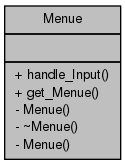
\includegraphics[width=166pt]{class_menue__coll__graph}
\end{center}
\end{figure}
\subsection*{Öffentliche Methoden}
\begin{DoxyCompactItemize}
\item 
void \hyperlink{class_menue_adab670791d2a103a26626b700698376d}{handle\-\_\-\-Input} (S\-D\-L\-\_\-\-Event \&\hyperlink{main_8cpp_af6a41c81a6372a814ffae9ba6615e1e7}{even}, bool $\ast$, bool $\ast$, \hyperlink{class_player}{Player} $\ast$temp)
\end{DoxyCompactItemize}
\subsection*{Öffentliche, statische Methoden}
\begin{DoxyCompactItemize}
\item 
static \hyperlink{class_menue}{Menue} \& \hyperlink{class_menue_a91bc6d5c4bb7214cd818223cdde9ef88}{get\-\_\-\-Menue} ()
\end{DoxyCompactItemize}


\subsection{Dokumentation der Elementfunktionen}
\hypertarget{class_menue_a91bc6d5c4bb7214cd818223cdde9ef88}{\index{Menue@{Menue}!get\-\_\-\-Menue@{get\-\_\-\-Menue}}
\index{get\-\_\-\-Menue@{get\-\_\-\-Menue}!Menue@{Menue}}
\subsubsection[{get\-\_\-\-Menue}]{\setlength{\rightskip}{0pt plus 5cm}{\bf Menue} \& Menue\-::get\-\_\-\-Menue (
\begin{DoxyParamCaption}
{}
\end{DoxyParamCaption}
)\hspace{0.3cm}{\ttfamily [static]}}}\label{class_menue_a91bc6d5c4bb7214cd818223cdde9ef88}


Hier ist ein Graph der zeigt, wo diese Funktion aufgerufen wird\-:
\nopagebreak
\begin{figure}[H]
\begin{center}
\leavevmode
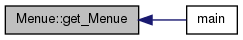
\includegraphics[width=254pt]{class_menue_a91bc6d5c4bb7214cd818223cdde9ef88_icgraph}
\end{center}
\end{figure}


\hypertarget{class_menue_adab670791d2a103a26626b700698376d}{\index{Menue@{Menue}!handle\-\_\-\-Input@{handle\-\_\-\-Input}}
\index{handle\-\_\-\-Input@{handle\-\_\-\-Input}!Menue@{Menue}}
\subsubsection[{handle\-\_\-\-Input}]{\setlength{\rightskip}{0pt plus 5cm}void Menue\-::handle\-\_\-\-Input (
\begin{DoxyParamCaption}
\item[{S\-D\-L\-\_\-\-Event \&}]{even, }
\item[{bool $\ast$}]{quitgame, }
\item[{bool $\ast$}]{quitmenue, }
\item[{{\bf Player} $\ast$}]{temp}
\end{DoxyParamCaption}
)}}\label{class_menue_adab670791d2a103a26626b700698376d}


Hier ist ein Graph, der zeigt, was diese Funktion aufruft\-:
\nopagebreak
\begin{figure}[H]
\begin{center}
\leavevmode
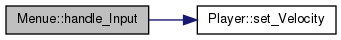
\includegraphics[width=328pt]{class_menue_adab670791d2a103a26626b700698376d_cgraph}
\end{center}
\end{figure}




Hier ist ein Graph der zeigt, wo diese Funktion aufgerufen wird\-:
\nopagebreak
\begin{figure}[H]
\begin{center}
\leavevmode
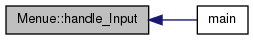
\includegraphics[width=262pt]{class_menue_adab670791d2a103a26626b700698376d_icgraph}
\end{center}
\end{figure}




Die Dokumentation für diese Klasse wurde erzeugt aufgrund der Dateien\-:\begin{DoxyCompactItemize}
\item 
\hyperlink{_menue_8h}{Menue.\-h}\item 
\hyperlink{_menue_8cpp}{Menue.\-cpp}\end{DoxyCompactItemize}

\hypertarget{class_money_manager}{\section{Money\-Manager Klassenreferenz}
\label{class_money_manager}\index{Money\-Manager@{Money\-Manager}}
}


{\ttfamily \#include $<$Money\-Manager.\-h$>$}



Zusammengehörigkeiten von Money\-Manager\-:
\nopagebreak
\begin{figure}[H]
\begin{center}
\leavevmode
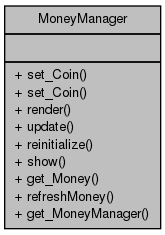
\includegraphics[width=196pt]{class_money_manager__coll__graph}
\end{center}
\end{figure}
\subsection*{Öffentliche Methoden}
\begin{DoxyCompactItemize}
\item 
void \hyperlink{class_money_manager_afb4cbbd62d99a50349450f994180a030}{set\-\_\-\-Coin} (\hyperlink{structs___vector}{s\-\_\-\-Vector} $\ast$p\-\_\-\-Temp\-Position)
\item 
void \hyperlink{class_money_manager_af86f1a7b7224997f693dae28a2e3b025}{set\-\_\-\-Coin} (int x, int y)
\item 
void \hyperlink{class_money_manager_a33ad5f3a0229855b500ccbaf791d48db}{render} (S\-D\-L\-\_\-\-Rect camera)
\item 
void \hyperlink{class_money_manager_a2732c50d4ab200fa9aa89881ddaafe9b}{update} (\hyperlink{structs___vector}{s\-\_\-\-Vector} $\ast$p\-\_\-\-Temp\-Position)
\item 
void \hyperlink{class_money_manager_ad48afb7b433b15f01a554884a0b2e086}{reinitialize} ()
\item 
void \hyperlink{class_money_manager_acec03aacba984985299507968b60c40b}{show} ()
\item 
int \hyperlink{class_money_manager_a4ded1a440c3c30ab5f1ff498aa1f0caf}{get\-\_\-\-Money} ()
\item 
int \hyperlink{class_money_manager_acda99c2efae55a5c4eaf5670305d7f07}{refresh\-Money} (int i\-\_\-bill)
\end{DoxyCompactItemize}
\subsection*{Öffentliche, statische Methoden}
\begin{DoxyCompactItemize}
\item 
static \hyperlink{class_money_manager}{Money\-Manager} \& \hyperlink{class_money_manager_a9e244a12805cbff0dee7f76d1ca8c05a}{get\-\_\-\-Money\-Manager} ()
\end{DoxyCompactItemize}
\subsection*{Private Methoden}
\begin{DoxyCompactItemize}
\item 
\hyperlink{class_money_manager_a7fad6a5fe1cf45b6d670b898ff5a54de}{Money\-Manager} ()
\item 
\hyperlink{class_money_manager_ac2a9e2cf428e0838a856724f2c442501}{$\sim$\-Money\-Manager} ()
\end{DoxyCompactItemize}
\subsection*{Private Attribute}
\begin{DoxyCompactItemize}
\item 
int \hyperlink{class_money_manager_aa396ea903542470a382c2054f1e40dd8}{money}
\item 
list$<$ \hyperlink{class_renable_object}{Renable\-Object} $>$ \hyperlink{class_money_manager_a803e15bb98cf698f1ad15da4c86f1194}{uncatchedmoney}
\end{DoxyCompactItemize}


\subsection{Beschreibung der Konstruktoren und Destruktoren}
\hypertarget{class_money_manager_a7fad6a5fe1cf45b6d670b898ff5a54de}{\index{Money\-Manager@{Money\-Manager}!Money\-Manager@{Money\-Manager}}
\index{Money\-Manager@{Money\-Manager}!MoneyManager@{Money\-Manager}}
\subsubsection[{Money\-Manager}]{\setlength{\rightskip}{0pt plus 5cm}Money\-Manager\-::\-Money\-Manager (
\begin{DoxyParamCaption}
{}
\end{DoxyParamCaption}
)\hspace{0.3cm}{\ttfamily [inline]}, {\ttfamily [private]}}}\label{class_money_manager_a7fad6a5fe1cf45b6d670b898ff5a54de}
\hypertarget{class_money_manager_ac2a9e2cf428e0838a856724f2c442501}{\index{Money\-Manager@{Money\-Manager}!$\sim$\-Money\-Manager@{$\sim$\-Money\-Manager}}
\index{$\sim$\-Money\-Manager@{$\sim$\-Money\-Manager}!MoneyManager@{Money\-Manager}}
\subsubsection[{$\sim$\-Money\-Manager}]{\setlength{\rightskip}{0pt plus 5cm}Money\-Manager\-::$\sim$\-Money\-Manager (
\begin{DoxyParamCaption}
{}
\end{DoxyParamCaption}
)\hspace{0.3cm}{\ttfamily [inline]}, {\ttfamily [private]}}}\label{class_money_manager_ac2a9e2cf428e0838a856724f2c442501}


\subsection{Dokumentation der Elementfunktionen}
\hypertarget{class_money_manager_a4ded1a440c3c30ab5f1ff498aa1f0caf}{\index{Money\-Manager@{Money\-Manager}!get\-\_\-\-Money@{get\-\_\-\-Money}}
\index{get\-\_\-\-Money@{get\-\_\-\-Money}!MoneyManager@{Money\-Manager}}
\subsubsection[{get\-\_\-\-Money}]{\setlength{\rightskip}{0pt plus 5cm}int Money\-Manager\-::get\-\_\-\-Money (
\begin{DoxyParamCaption}
{}
\end{DoxyParamCaption}
)\hspace{0.3cm}{\ttfamily [inline]}}}\label{class_money_manager_a4ded1a440c3c30ab5f1ff498aa1f0caf}


Hier ist ein Graph der zeigt, wo diese Funktion aufgerufen wird\-:\nopagebreak
\begin{figure}[H]
\begin{center}
\leavevmode
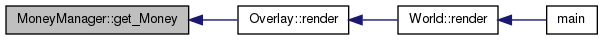
\includegraphics[width=350pt]{class_money_manager_a4ded1a440c3c30ab5f1ff498aa1f0caf_icgraph}
\end{center}
\end{figure}


\hypertarget{class_money_manager_a9e244a12805cbff0dee7f76d1ca8c05a}{\index{Money\-Manager@{Money\-Manager}!get\-\_\-\-Money\-Manager@{get\-\_\-\-Money\-Manager}}
\index{get\-\_\-\-Money\-Manager@{get\-\_\-\-Money\-Manager}!MoneyManager@{Money\-Manager}}
\subsubsection[{get\-\_\-\-Money\-Manager}]{\setlength{\rightskip}{0pt plus 5cm}static {\bf Money\-Manager}\& Money\-Manager\-::get\-\_\-\-Money\-Manager (
\begin{DoxyParamCaption}
{}
\end{DoxyParamCaption}
)\hspace{0.3cm}{\ttfamily [inline]}, {\ttfamily [static]}}}\label{class_money_manager_a9e244a12805cbff0dee7f76d1ca8c05a}


Hier ist ein Graph der zeigt, wo diese Funktion aufgerufen wird\-:\nopagebreak
\begin{figure}[H]
\begin{center}
\leavevmode
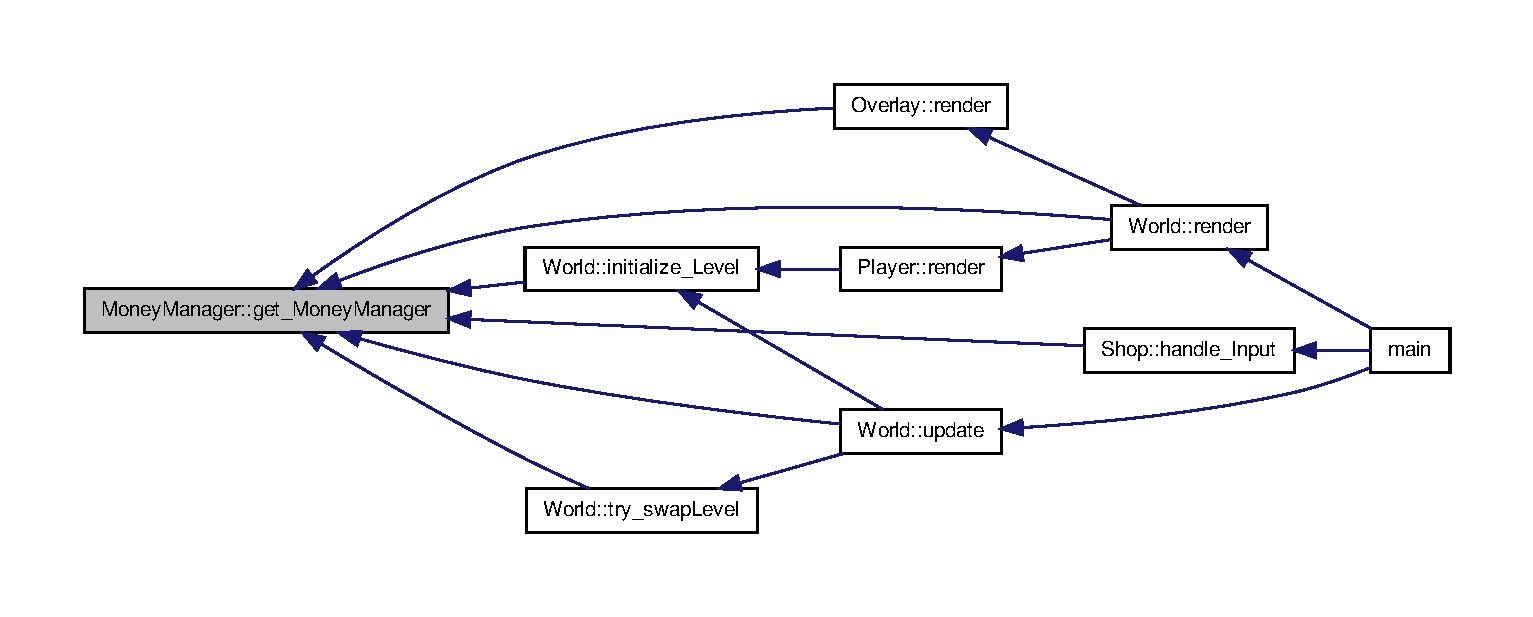
\includegraphics[width=350pt]{class_money_manager_a9e244a12805cbff0dee7f76d1ca8c05a_icgraph}
\end{center}
\end{figure}


\hypertarget{class_money_manager_acda99c2efae55a5c4eaf5670305d7f07}{\index{Money\-Manager@{Money\-Manager}!refresh\-Money@{refresh\-Money}}
\index{refresh\-Money@{refresh\-Money}!MoneyManager@{Money\-Manager}}
\subsubsection[{refresh\-Money}]{\setlength{\rightskip}{0pt plus 5cm}int Money\-Manager\-::refresh\-Money (
\begin{DoxyParamCaption}
\item[{int}]{i\-\_\-bill}
\end{DoxyParamCaption}
)}}\label{class_money_manager_acda99c2efae55a5c4eaf5670305d7f07}


Hier ist ein Graph der zeigt, wo diese Funktion aufgerufen wird\-:\nopagebreak
\begin{figure}[H]
\begin{center}
\leavevmode
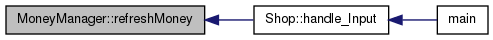
\includegraphics[width=350pt]{class_money_manager_acda99c2efae55a5c4eaf5670305d7f07_icgraph}
\end{center}
\end{figure}


\hypertarget{class_money_manager_ad48afb7b433b15f01a554884a0b2e086}{\index{Money\-Manager@{Money\-Manager}!reinitialize@{reinitialize}}
\index{reinitialize@{reinitialize}!MoneyManager@{Money\-Manager}}
\subsubsection[{reinitialize}]{\setlength{\rightskip}{0pt plus 5cm}void Money\-Manager\-::reinitialize (
\begin{DoxyParamCaption}
{}
\end{DoxyParamCaption}
)\hspace{0.3cm}{\ttfamily [inline]}}}\label{class_money_manager_ad48afb7b433b15f01a554884a0b2e086}


Hier ist ein Graph der zeigt, wo diese Funktion aufgerufen wird\-:\nopagebreak
\begin{figure}[H]
\begin{center}
\leavevmode
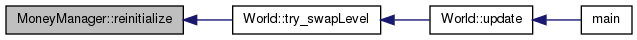
\includegraphics[width=350pt]{class_money_manager_ad48afb7b433b15f01a554884a0b2e086_icgraph}
\end{center}
\end{figure}


\hypertarget{class_money_manager_a33ad5f3a0229855b500ccbaf791d48db}{\index{Money\-Manager@{Money\-Manager}!render@{render}}
\index{render@{render}!MoneyManager@{Money\-Manager}}
\subsubsection[{render}]{\setlength{\rightskip}{0pt plus 5cm}void Money\-Manager\-::render (
\begin{DoxyParamCaption}
\item[{S\-D\-L\-\_\-\-Rect}]{camera}
\end{DoxyParamCaption}
)}}\label{class_money_manager_a33ad5f3a0229855b500ccbaf791d48db}


Hier ist ein Graph, der zeigt, was diese Funktion aufruft\-:\nopagebreak
\begin{figure}[H]
\begin{center}
\leavevmode
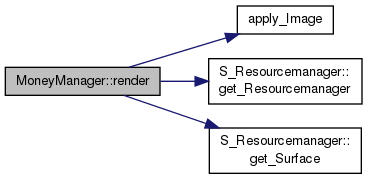
\includegraphics[width=348pt]{class_money_manager_a33ad5f3a0229855b500ccbaf791d48db_cgraph}
\end{center}
\end{figure}




Hier ist ein Graph der zeigt, wo diese Funktion aufgerufen wird\-:\nopagebreak
\begin{figure}[H]
\begin{center}
\leavevmode
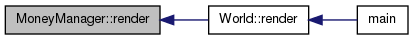
\includegraphics[width=350pt]{class_money_manager_a33ad5f3a0229855b500ccbaf791d48db_icgraph}
\end{center}
\end{figure}


\hypertarget{class_money_manager_afb4cbbd62d99a50349450f994180a030}{\index{Money\-Manager@{Money\-Manager}!set\-\_\-\-Coin@{set\-\_\-\-Coin}}
\index{set\-\_\-\-Coin@{set\-\_\-\-Coin}!MoneyManager@{Money\-Manager}}
\subsubsection[{set\-\_\-\-Coin}]{\setlength{\rightskip}{0pt plus 5cm}void Money\-Manager\-::set\-\_\-\-Coin (
\begin{DoxyParamCaption}
\item[{{\bf s\-\_\-\-Vector} $\ast$}]{p\-\_\-\-Temp\-Position}
\end{DoxyParamCaption}
)}}\label{class_money_manager_afb4cbbd62d99a50349450f994180a030}


Hier ist ein Graph der zeigt, wo diese Funktion aufgerufen wird\-:\nopagebreak
\begin{figure}[H]
\begin{center}
\leavevmode
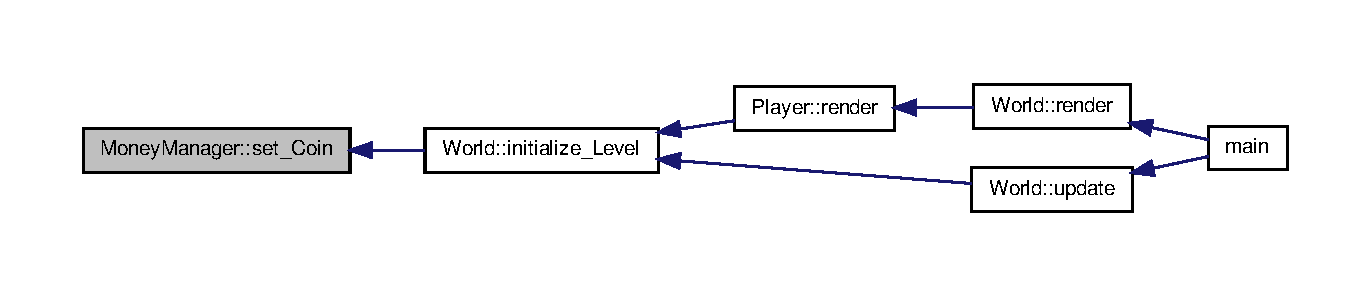
\includegraphics[width=350pt]{class_money_manager_afb4cbbd62d99a50349450f994180a030_icgraph}
\end{center}
\end{figure}


\hypertarget{class_money_manager_af86f1a7b7224997f693dae28a2e3b025}{\index{Money\-Manager@{Money\-Manager}!set\-\_\-\-Coin@{set\-\_\-\-Coin}}
\index{set\-\_\-\-Coin@{set\-\_\-\-Coin}!MoneyManager@{Money\-Manager}}
\subsubsection[{set\-\_\-\-Coin}]{\setlength{\rightskip}{0pt plus 5cm}void Money\-Manager\-::set\-\_\-\-Coin (
\begin{DoxyParamCaption}
\item[{int}]{x, }
\item[{int}]{y}
\end{DoxyParamCaption}
)}}\label{class_money_manager_af86f1a7b7224997f693dae28a2e3b025}
\hypertarget{class_money_manager_acec03aacba984985299507968b60c40b}{\index{Money\-Manager@{Money\-Manager}!show@{show}}
\index{show@{show}!MoneyManager@{Money\-Manager}}
\subsubsection[{show}]{\setlength{\rightskip}{0pt plus 5cm}void Money\-Manager\-::show (
\begin{DoxyParamCaption}
{}
\end{DoxyParamCaption}
)\hspace{0.3cm}{\ttfamily [inline]}}}\label{class_money_manager_acec03aacba984985299507968b60c40b}
\hypertarget{class_money_manager_a2732c50d4ab200fa9aa89881ddaafe9b}{\index{Money\-Manager@{Money\-Manager}!update@{update}}
\index{update@{update}!MoneyManager@{Money\-Manager}}
\subsubsection[{update}]{\setlength{\rightskip}{0pt plus 5cm}void Money\-Manager\-::update (
\begin{DoxyParamCaption}
\item[{{\bf s\-\_\-\-Vector} $\ast$}]{p\-\_\-\-Temp\-Position}
\end{DoxyParamCaption}
)}}\label{class_money_manager_a2732c50d4ab200fa9aa89881ddaafe9b}


Hier ist ein Graph, der zeigt, was diese Funktion aufruft\-:\nopagebreak
\begin{figure}[H]
\begin{center}
\leavevmode
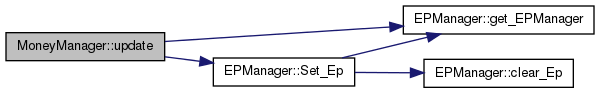
\includegraphics[width=350pt]{class_money_manager_a2732c50d4ab200fa9aa89881ddaafe9b_cgraph}
\end{center}
\end{figure}




Hier ist ein Graph der zeigt, wo diese Funktion aufgerufen wird\-:\nopagebreak
\begin{figure}[H]
\begin{center}
\leavevmode
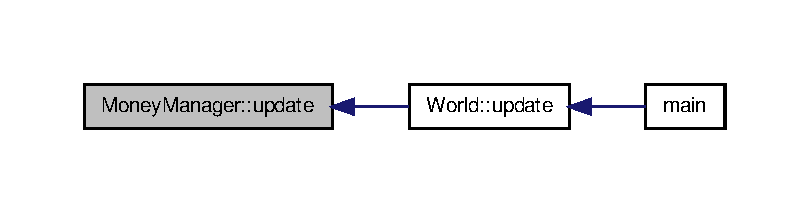
\includegraphics[width=350pt]{class_money_manager_a2732c50d4ab200fa9aa89881ddaafe9b_icgraph}
\end{center}
\end{figure}




\subsection{Dokumentation der Datenelemente}
\hypertarget{class_money_manager_aa396ea903542470a382c2054f1e40dd8}{\index{Money\-Manager@{Money\-Manager}!money@{money}}
\index{money@{money}!MoneyManager@{Money\-Manager}}
\subsubsection[{money}]{\setlength{\rightskip}{0pt plus 5cm}int Money\-Manager\-::money\hspace{0.3cm}{\ttfamily [private]}}}\label{class_money_manager_aa396ea903542470a382c2054f1e40dd8}
\hypertarget{class_money_manager_a803e15bb98cf698f1ad15da4c86f1194}{\index{Money\-Manager@{Money\-Manager}!uncatchedmoney@{uncatchedmoney}}
\index{uncatchedmoney@{uncatchedmoney}!MoneyManager@{Money\-Manager}}
\subsubsection[{uncatchedmoney}]{\setlength{\rightskip}{0pt plus 5cm}list$<${\bf Renable\-Object}$>$ Money\-Manager\-::uncatchedmoney\hspace{0.3cm}{\ttfamily [private]}}}\label{class_money_manager_a803e15bb98cf698f1ad15da4c86f1194}


Die Dokumentation für diese Klasse wurde erzeugt aufgrund der Dateien\-:\begin{DoxyCompactItemize}
\item 
\hyperlink{_money_manager_8h}{Money\-Manager.\-h}\item 
\hyperlink{_money_manager_8cpp}{Money\-Manager.\-cpp}\end{DoxyCompactItemize}

\hypertarget{class_n_p_c1}{\section{N\-P\-C1 Klassenreferenz}
\label{class_n_p_c1}\index{N\-P\-C1@{N\-P\-C1}}
}


{\ttfamily \#include $<$N\-P\-C1.\-h$>$}



Zusammengehörigkeiten von N\-P\-C1\-:
\nopagebreak
\begin{figure}[H]
\begin{center}
\leavevmode
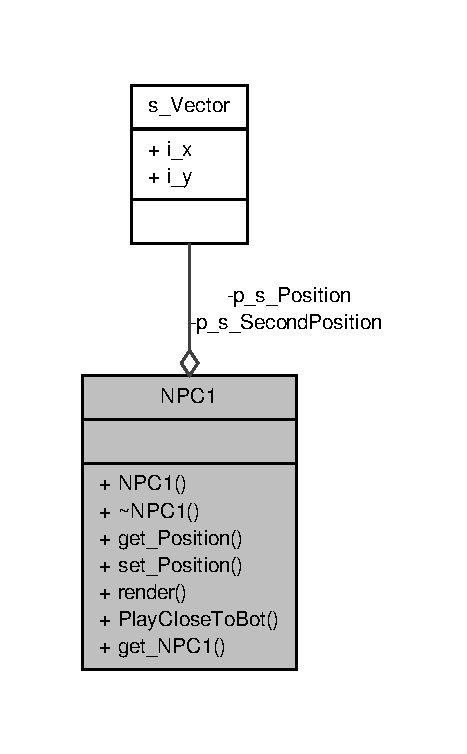
\includegraphics[width=182pt]{class_n_p_c1__coll__graph}
\end{center}
\end{figure}
\subsection*{Öffentliche Methoden}
\begin{DoxyCompactItemize}
\item 
\hyperlink{class_n_p_c1_ad76416c9a95fb9a774976297c8593595}{N\-P\-C1} ()
\item 
\hyperlink{class_n_p_c1_ab204b325bcd16659c66a491c9b10e8e2}{$\sim$\-N\-P\-C1} ()
\item 
\hyperlink{structs___vector}{s\-\_\-\-Vector} $\ast$ \hyperlink{class_n_p_c1_aa76eead3904b61145d210ee5d077fab9}{get\-\_\-\-Position} ()
\item 
void \hyperlink{class_n_p_c1_a6f7d2842c3ad04969ed90722324875b4}{set\-\_\-\-Position} (int i\-\_\-x, int i\-\_\-y)
\item 
void \hyperlink{class_n_p_c1_a3fa4f42017cbef90df3fc010de47f452}{render} (S\-D\-L\-\_\-\-Rect camera)
\item 
bool \hyperlink{class_n_p_c1_a630634825b51471ec57664e03f8f69c1}{Play\-Close\-To\-Bot} (\hyperlink{class_player}{Player} $\ast$p\-\_\-\-Temp\-Player)
\end{DoxyCompactItemize}
\subsection*{Öffentliche, statische Methoden}
\begin{DoxyCompactItemize}
\item 
static \hyperlink{class_n_p_c1}{N\-P\-C1} \& \hyperlink{class_n_p_c1_aa44be35612f75bcfb437dc5277f63b57}{get\-\_\-\-N\-P\-C1} ()
\end{DoxyCompactItemize}


\subsection{Beschreibung der Konstruktoren und Destruktoren}
\hypertarget{class_n_p_c1_ad76416c9a95fb9a774976297c8593595}{\index{N\-P\-C1@{N\-P\-C1}!N\-P\-C1@{N\-P\-C1}}
\index{N\-P\-C1@{N\-P\-C1}!NPC1@{N\-P\-C1}}
\subsubsection[{N\-P\-C1}]{\setlength{\rightskip}{0pt plus 5cm}N\-P\-C1\-::\-N\-P\-C1 (
\begin{DoxyParamCaption}
{}
\end{DoxyParamCaption}
)\hspace{0.3cm}{\ttfamily [inline]}}}\label{class_n_p_c1_ad76416c9a95fb9a774976297c8593595}
\hypertarget{class_n_p_c1_ab204b325bcd16659c66a491c9b10e8e2}{\index{N\-P\-C1@{N\-P\-C1}!$\sim$\-N\-P\-C1@{$\sim$\-N\-P\-C1}}
\index{$\sim$\-N\-P\-C1@{$\sim$\-N\-P\-C1}!NPC1@{N\-P\-C1}}
\subsubsection[{$\sim$\-N\-P\-C1}]{\setlength{\rightskip}{0pt plus 5cm}N\-P\-C1\-::$\sim$\-N\-P\-C1 (
\begin{DoxyParamCaption}
{}
\end{DoxyParamCaption}
)\hspace{0.3cm}{\ttfamily [inline]}}}\label{class_n_p_c1_ab204b325bcd16659c66a491c9b10e8e2}


\subsection{Dokumentation der Elementfunktionen}
\hypertarget{class_n_p_c1_aa44be35612f75bcfb437dc5277f63b57}{\index{N\-P\-C1@{N\-P\-C1}!get\-\_\-\-N\-P\-C1@{get\-\_\-\-N\-P\-C1}}
\index{get\-\_\-\-N\-P\-C1@{get\-\_\-\-N\-P\-C1}!NPC1@{N\-P\-C1}}
\subsubsection[{get\-\_\-\-N\-P\-C1}]{\setlength{\rightskip}{0pt plus 5cm}static {\bf N\-P\-C1}\& N\-P\-C1\-::get\-\_\-\-N\-P\-C1 (
\begin{DoxyParamCaption}
{}
\end{DoxyParamCaption}
)\hspace{0.3cm}{\ttfamily [inline]}, {\ttfamily [static]}}}\label{class_n_p_c1_aa44be35612f75bcfb437dc5277f63b57}


Hier ist ein Graph der zeigt, wo diese Funktion aufgerufen wird\-:
\nopagebreak
\begin{figure}[H]
\begin{center}
\leavevmode
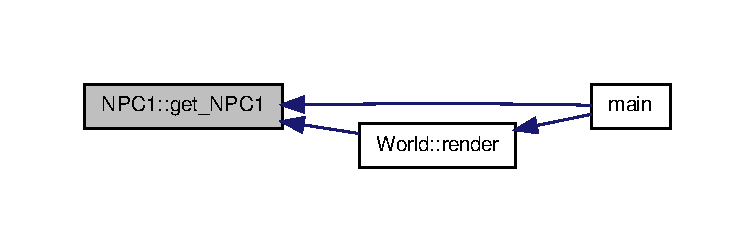
\includegraphics[width=350pt]{class_n_p_c1_aa44be35612f75bcfb437dc5277f63b57_icgraph}
\end{center}
\end{figure}


\hypertarget{class_n_p_c1_aa76eead3904b61145d210ee5d077fab9}{\index{N\-P\-C1@{N\-P\-C1}!get\-\_\-\-Position@{get\-\_\-\-Position}}
\index{get\-\_\-\-Position@{get\-\_\-\-Position}!NPC1@{N\-P\-C1}}
\subsubsection[{get\-\_\-\-Position}]{\setlength{\rightskip}{0pt plus 5cm}{\bf s\-\_\-\-Vector}$\ast$ N\-P\-C1\-::get\-\_\-\-Position (
\begin{DoxyParamCaption}
{}
\end{DoxyParamCaption}
)\hspace{0.3cm}{\ttfamily [inline]}}}\label{class_n_p_c1_aa76eead3904b61145d210ee5d077fab9}
\hypertarget{class_n_p_c1_a630634825b51471ec57664e03f8f69c1}{\index{N\-P\-C1@{N\-P\-C1}!Play\-Close\-To\-Bot@{Play\-Close\-To\-Bot}}
\index{Play\-Close\-To\-Bot@{Play\-Close\-To\-Bot}!NPC1@{N\-P\-C1}}
\subsubsection[{Play\-Close\-To\-Bot}]{\setlength{\rightskip}{0pt plus 5cm}bool N\-P\-C1\-::\-Play\-Close\-To\-Bot (
\begin{DoxyParamCaption}
\item[{{\bf Player} $\ast$}]{p\-\_\-\-Temp\-Player}
\end{DoxyParamCaption}
)}}\label{class_n_p_c1_a630634825b51471ec57664e03f8f69c1}


Hier ist ein Graph, der zeigt, was diese Funktion aufruft\-:
\nopagebreak
\begin{figure}[H]
\begin{center}
\leavevmode
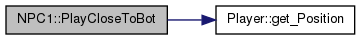
\includegraphics[width=342pt]{class_n_p_c1_a630634825b51471ec57664e03f8f69c1_cgraph}
\end{center}
\end{figure}




Hier ist ein Graph der zeigt, wo diese Funktion aufgerufen wird\-:
\nopagebreak
\begin{figure}[H]
\begin{center}
\leavevmode
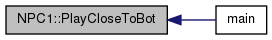
\includegraphics[width=276pt]{class_n_p_c1_a630634825b51471ec57664e03f8f69c1_icgraph}
\end{center}
\end{figure}


\hypertarget{class_n_p_c1_a3fa4f42017cbef90df3fc010de47f452}{\index{N\-P\-C1@{N\-P\-C1}!render@{render}}
\index{render@{render}!NPC1@{N\-P\-C1}}
\subsubsection[{render}]{\setlength{\rightskip}{0pt plus 5cm}void N\-P\-C1\-::render (
\begin{DoxyParamCaption}
\item[{S\-D\-L\-\_\-\-Rect}]{camera}
\end{DoxyParamCaption}
)}}\label{class_n_p_c1_a3fa4f42017cbef90df3fc010de47f452}


Hier ist ein Graph, der zeigt, was diese Funktion aufruft\-:
\nopagebreak
\begin{figure}[H]
\begin{center}
\leavevmode
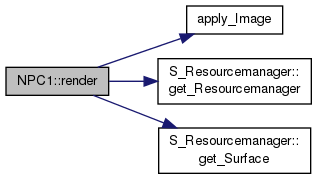
\includegraphics[width=310pt]{class_n_p_c1_a3fa4f42017cbef90df3fc010de47f452_cgraph}
\end{center}
\end{figure}




Hier ist ein Graph der zeigt, wo diese Funktion aufgerufen wird\-:
\nopagebreak
\begin{figure}[H]
\begin{center}
\leavevmode
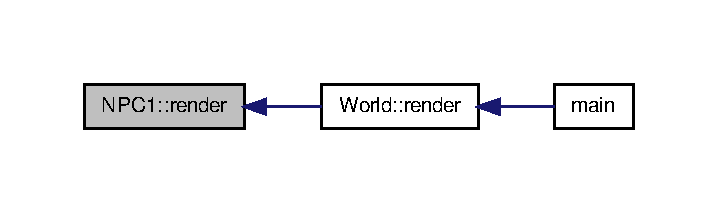
\includegraphics[width=344pt]{class_n_p_c1_a3fa4f42017cbef90df3fc010de47f452_icgraph}
\end{center}
\end{figure}


\hypertarget{class_n_p_c1_a6f7d2842c3ad04969ed90722324875b4}{\index{N\-P\-C1@{N\-P\-C1}!set\-\_\-\-Position@{set\-\_\-\-Position}}
\index{set\-\_\-\-Position@{set\-\_\-\-Position}!NPC1@{N\-P\-C1}}
\subsubsection[{set\-\_\-\-Position}]{\setlength{\rightskip}{0pt plus 5cm}void N\-P\-C1\-::set\-\_\-\-Position (
\begin{DoxyParamCaption}
\item[{int}]{i\-\_\-x, }
\item[{int}]{i\-\_\-y}
\end{DoxyParamCaption}
)\hspace{0.3cm}{\ttfamily [inline]}}}\label{class_n_p_c1_a6f7d2842c3ad04969ed90722324875b4}


Die Dokumentation für diese Klasse wurde erzeugt aufgrund der Dateien\-:\begin{DoxyCompactItemize}
\item 
\hyperlink{_n_p_c1_8h}{N\-P\-C1.\-h}\item 
\hyperlink{_n_p_c1_8cpp}{N\-P\-C1.\-cpp}\end{DoxyCompactItemize}

\hypertarget{class_n_p_c2}{\section{N\-P\-C2 Klassenreferenz}
\label{class_n_p_c2}\index{N\-P\-C2@{N\-P\-C2}}
}
\subsection*{Öffentliche Methoden}
\begin{DoxyCompactItemize}
\item 
\hypertarget{class_n_p_c2_a8dbd0f944b51a7d6acb0f4faf3f7eb92}{\hyperlink{structs___vector}{s\-\_\-\-Vector} $\ast$ {\bfseries get\-\_\-\-Position} ()}\label{class_n_p_c2_a8dbd0f944b51a7d6acb0f4faf3f7eb92}

\item 
\hypertarget{class_n_p_c2_a77cbb553e517b11026e95cf7f0ada3d6}{void {\bfseries set\-\_\-\-Position} (int i\-\_\-x, int i\-\_\-y)}\label{class_n_p_c2_a77cbb553e517b11026e95cf7f0ada3d6}

\item 
\hypertarget{class_n_p_c2_a5f05d6eaecaaa39e744569b453fd0c05}{void {\bfseries render} (S\-D\-L\-\_\-\-Rect camera)}\label{class_n_p_c2_a5f05d6eaecaaa39e744569b453fd0c05}

\item 
\hypertarget{class_n_p_c2_abd040a952f1ca623263fb4981d9f1897}{bool {\bfseries Play\-Close\-To\-Bot} (\hyperlink{class_player}{Player} $\ast$p\-\_\-\-Temp\-Player)}\label{class_n_p_c2_abd040a952f1ca623263fb4981d9f1897}

\end{DoxyCompactItemize}
\subsection*{Öffentliche, statische Methoden}
\begin{DoxyCompactItemize}
\item 
\hypertarget{class_n_p_c2_af885f9c5210936ba28c99d2c23971595}{static \hyperlink{class_n_p_c2}{N\-P\-C2} \& {\bfseries get\-\_\-\-N\-P\-C2} ()}\label{class_n_p_c2_af885f9c5210936ba28c99d2c23971595}

\end{DoxyCompactItemize}


Die Dokumentation für diese Klasse wurde erzeugt aufgrund der Dateien\-:\begin{DoxyCompactItemize}
\item 
N\-P\-C2.\-h\item 
N\-P\-C2.\-cpp\end{DoxyCompactItemize}

\hypertarget{class_n_p_c_manager}{\section{N\-P\-C\-Manager Klassenreferenz}
\label{class_n_p_c_manager}\index{N\-P\-C\-Manager@{N\-P\-C\-Manager}}
}


{\ttfamily \#include $<$N\-P\-C\-Manager.\-h$>$}



Zusammengehörigkeiten von N\-P\-C\-Manager\-:
\nopagebreak
\begin{figure}[H]
\begin{center}
\leavevmode
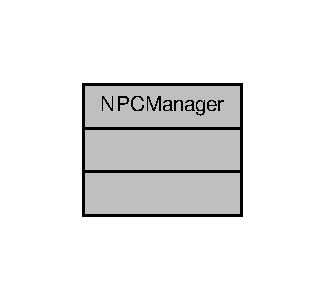
\includegraphics[width=156pt]{class_n_p_c_manager__coll__graph}
\end{center}
\end{figure}


Die Dokumentation für diese Klasse wurde erzeugt aufgrund der Datei\-:\begin{DoxyCompactItemize}
\item 
\hyperlink{_n_p_c_manager_8h}{N\-P\-C\-Manager.\-h}\end{DoxyCompactItemize}

\hypertarget{class_overlay}{\section{Overlay Klassenreferenz}
\label{class_overlay}\index{Overlay@{Overlay}}
}


Hier wird der gesamte status des Spielers auf den screen gebracht.  




{\ttfamily \#include $<$Overlay.\-h$>$}



Zusammengehörigkeiten von Overlay\-:
\nopagebreak
\begin{figure}[H]
\begin{center}
\leavevmode
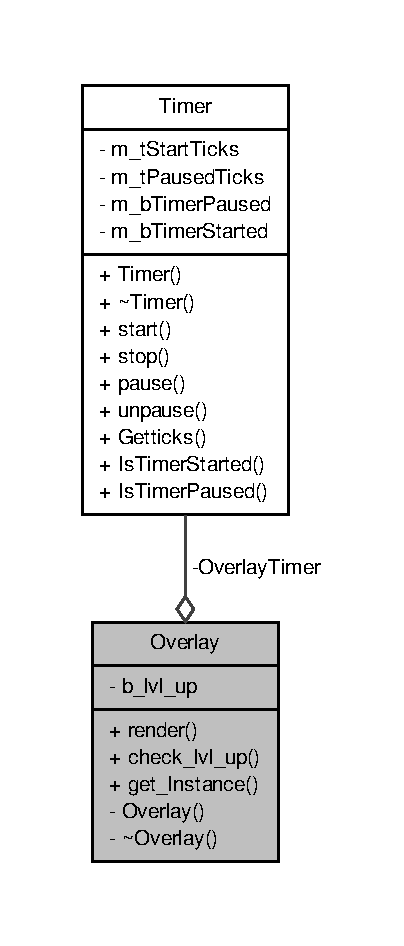
\includegraphics[width=168pt]{class_overlay__coll__graph}
\end{center}
\end{figure}
\subsection*{Öffentliche Methoden}
\begin{DoxyCompactItemize}
\item 
void \hyperlink{class_overlay_ab5e47eefa2743c08bc208131c8b17a45}{render} (\hyperlink{class_player}{Player} $\ast$p\-\_\-\-Temp\-Player)
\item 
void \hyperlink{class_overlay_a6e01bd776bf1daf819ced8e0e45b4478}{check\-\_\-lvl\-\_\-up} ()
\end{DoxyCompactItemize}
\subsection*{Öffentliche, statische Methoden}
\begin{DoxyCompactItemize}
\item 
static \hyperlink{class_overlay}{Overlay} \& \hyperlink{class_overlay_a6f0ea07b818fdc4ea2b00f1ed8169a6f}{get\-\_\-\-Instance} ()
\end{DoxyCompactItemize}


\subsection{Ausführliche Beschreibung}
Hier wird der gesamte status des Spielers auf den screen gebracht. 

\subsection{Dokumentation der Elementfunktionen}
\hypertarget{class_overlay_a6e01bd776bf1daf819ced8e0e45b4478}{\index{Overlay@{Overlay}!check\-\_\-lvl\-\_\-up@{check\-\_\-lvl\-\_\-up}}
\index{check\-\_\-lvl\-\_\-up@{check\-\_\-lvl\-\_\-up}!Overlay@{Overlay}}
\subsubsection[{check\-\_\-lvl\-\_\-up}]{\setlength{\rightskip}{0pt plus 5cm}void Overlay\-::check\-\_\-lvl\-\_\-up (
\begin{DoxyParamCaption}
{}
\end{DoxyParamCaption}
)}}\label{class_overlay_a6e01bd776bf1daf819ced8e0e45b4478}


Hier ist ein Graph, der zeigt, was diese Funktion aufruft\-:
\nopagebreak
\begin{figure}[H]
\begin{center}
\leavevmode
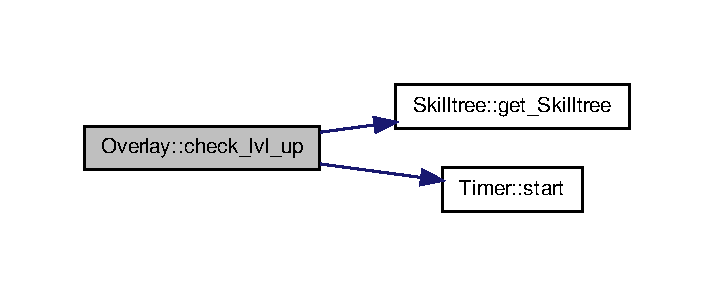
\includegraphics[width=342pt]{class_overlay_a6e01bd776bf1daf819ced8e0e45b4478_cgraph}
\end{center}
\end{figure}




Hier ist ein Graph der zeigt, wo diese Funktion aufgerufen wird\-:
\nopagebreak
\begin{figure}[H]
\begin{center}
\leavevmode
\includegraphics[width=268pt]{class_overlay_a6e01bd776bf1daf819ced8e0e45b4478_icgraph}
\end{center}
\end{figure}


\hypertarget{class_overlay_a6f0ea07b818fdc4ea2b00f1ed8169a6f}{\index{Overlay@{Overlay}!get\-\_\-\-Instance@{get\-\_\-\-Instance}}
\index{get\-\_\-\-Instance@{get\-\_\-\-Instance}!Overlay@{Overlay}}
\subsubsection[{get\-\_\-\-Instance}]{\setlength{\rightskip}{0pt plus 5cm}static {\bf Overlay}\& Overlay\-::get\-\_\-\-Instance (
\begin{DoxyParamCaption}
{}
\end{DoxyParamCaption}
)\hspace{0.3cm}{\ttfamily [inline]}, {\ttfamily [static]}}}\label{class_overlay_a6f0ea07b818fdc4ea2b00f1ed8169a6f}


Hier ist ein Graph der zeigt, wo diese Funktion aufgerufen wird\-:
\nopagebreak
\begin{figure}[H]
\begin{center}
\leavevmode
\includegraphics[width=350pt]{class_overlay_a6f0ea07b818fdc4ea2b00f1ed8169a6f_icgraph}
\end{center}
\end{figure}


\hypertarget{class_overlay_ab5e47eefa2743c08bc208131c8b17a45}{\index{Overlay@{Overlay}!render@{render}}
\index{render@{render}!Overlay@{Overlay}}
\subsubsection[{render}]{\setlength{\rightskip}{0pt plus 5cm}void Overlay\-::render (
\begin{DoxyParamCaption}
\item[{{\bf Player} $\ast$}]{p\-\_\-\-Temp\-Player}
\end{DoxyParamCaption}
)}}\label{class_overlay_ab5e47eefa2743c08bc208131c8b17a45}
Malen die Leben des Spielers auf den Bildschirm 

Hier ist ein Graph, der zeigt, was diese Funktion aufruft\-:
\nopagebreak
\begin{figure}[H]
\begin{center}
\leavevmode
\includegraphics[width=350pt]{class_overlay_ab5e47eefa2743c08bc208131c8b17a45_cgraph}
\end{center}
\end{figure}




Hier ist ein Graph der zeigt, wo diese Funktion aufgerufen wird\-:
\nopagebreak
\begin{figure}[H]
\begin{center}
\leavevmode
\includegraphics[width=350pt]{class_overlay_ab5e47eefa2743c08bc208131c8b17a45_icgraph}
\end{center}
\end{figure}




Die Dokumentation für diese Klasse wurde erzeugt aufgrund der Dateien\-:\begin{DoxyCompactItemize}
\item 
\hyperlink{_overlay_8h}{Overlay.\-h}\item 
\hyperlink{_overlay_8cpp}{Overlay.\-cpp}\end{DoxyCompactItemize}

\hypertarget{class_pfleger}{\section{Pfleger Klassenreferenz}
\label{class_pfleger}\index{Pfleger@{Pfleger}}
}


Diese Klasse erstellt einen Spritzenschie�enden Gegner, die \hyperlink{class_spritze}{Spritze} ist dabei ein eigenes Objekt und testet K\-Ollision selbst.  




{\ttfamily \#include $<$Pfleger.\-h$>$}

\subsection*{Öffentliche Methoden}
\begin{DoxyCompactItemize}
\item 
\hypertarget{class_pfleger_a26093400c124cd80c3905aed358f3613}{{\bfseries Pfleger} (int x, int y)}\label{class_pfleger_a26093400c124cd80c3905aed358f3613}

\item 
\hypertarget{class_pfleger_a8af1eb8290c18f38547cab4182fd9801}{\hyperlink{structs___vector}{s\-\_\-\-Vector} $\ast$ {\bfseries get\-\_\-\-Position} ()}\label{class_pfleger_a8af1eb8290c18f38547cab4182fd9801}

\item 
\hypertarget{class_pfleger_a125d4f58e1d558e3da1632f5b145c981}{void {\bfseries set\-\_\-\-Position} (int x, int y)}\label{class_pfleger_a125d4f58e1d558e3da1632f5b145c981}

\item 
\hypertarget{class_pfleger_aa6c0976c738b053ac48086c47f0ecebb}{\hyperlink{class_timer}{Timer} $\ast$ {\bfseries get\-\_\-\-Timer} ()}\label{class_pfleger_aa6c0976c738b053ac48086c47f0ecebb}

\item 
\hypertarget{class_pfleger_ab16f8907843415401742d8def572da73}{void {\bfseries update} (\hyperlink{class_player}{Player} $\ast$p\-\_\-\-Temp\-Player)}\label{class_pfleger_ab16f8907843415401742d8def572da73}

\item 
\hypertarget{class_pfleger_a4ae72e0182e9d909358755769447681d}{void {\bfseries render} (S\-D\-L\-\_\-\-Rect camera)}\label{class_pfleger_a4ae72e0182e9d909358755769447681d}

\end{DoxyCompactItemize}


\subsection{Ausführliche Beschreibung}
Diese Klasse erstellt einen Spritzenschie�enden Gegner, die \hyperlink{class_spritze}{Spritze} ist dabei ein eigenes Objekt und testet K\-Ollision selbst. 

Die Dokumentation für diese Klasse wurde erzeugt aufgrund der Dateien\-:\begin{DoxyCompactItemize}
\item 
Pfleger.\-h\item 
Pfleger.\-cpp\end{DoxyCompactItemize}

\hypertarget{class_player}{\section{Player Klassenreferenz}
\label{class_player}\index{Player@{Player}}
}
\subsection*{Öffentliche Methoden}
\begin{DoxyCompactItemize}
\item 
\hypertarget{class_player_aa87d00dbf49b8d4fa4eb22d1351a7663}{{\bfseries Player} (int i\-\_\-x, int i\-\_\-y)}\label{class_player_aa87d00dbf49b8d4fa4eb22d1351a7663}

\item 
\hypertarget{class_player_a50f12c89f28826db8191f76ed915d788}{\hyperlink{structs___vector}{s\-\_\-\-Vector} $\ast$ {\bfseries get\-\_\-\-Position} ()}\label{class_player_a50f12c89f28826db8191f76ed915d788}

\item 
\hypertarget{class_player_a3615907f803845ff9b37dee94944b09b}{void {\bfseries set\-\_\-\-Position} (int i\-\_\-x, int i\-\_\-y)}\label{class_player_a3615907f803845ff9b37dee94944b09b}

\item 
\hypertarget{class_player_a0b3564dce7078dee4733a2af2460fae1}{\hyperlink{structs___vector}{s\-\_\-\-Vector} $\ast$ {\bfseries get\-\_\-\-Velocity} ()}\label{class_player_a0b3564dce7078dee4733a2af2460fae1}

\item 
\hypertarget{class_player_a12fea44fe4eda565ada463b15443dc56}{void {\bfseries set\-\_\-\-Velocity} (int i\-\_\-x, int i\-\_\-y)}\label{class_player_a12fea44fe4eda565ada463b15443dc56}

\item 
\hypertarget{class_player_a25da073f8c291a56b482d8005b2476d1}{void {\bfseries set\-\_\-\-Health} (int health)}\label{class_player_a25da073f8c291a56b482d8005b2476d1}

\item 
\hypertarget{class_player_af0ddd345e35423723ce460c64cd9a7b6}{void {\bfseries set\-\_\-\-Mana} (int mana)}\label{class_player_af0ddd345e35423723ce460c64cd9a7b6}

\item 
\hypertarget{class_player_a8684c93430c1a9d3827071e00bcdc0d2}{int {\bfseries get\-\_\-\-Health} () const }\label{class_player_a8684c93430c1a9d3827071e00bcdc0d2}

\item 
\hypertarget{class_player_a352a8894a05f649fb236ae99cd9da3e9}{int {\bfseries get\-\_\-\-Mana} () const }\label{class_player_a352a8894a05f649fb236ae99cd9da3e9}

\item 
\hypertarget{class_player_a20ab0b8731172d9b39989b1700ebd47d}{bool {\bfseries get\-\_\-disable} ()}\label{class_player_a20ab0b8731172d9b39989b1700ebd47d}

\item 
\hypertarget{class_player_add9dfdb430f9e78178e43a8bf78fa7a3}{void {\bfseries set\-\_\-disable} (bool t)}\label{class_player_add9dfdb430f9e78178e43a8bf78fa7a3}

\item 
\hypertarget{class_player_ae2b606a4cc6b7f3f1147c117fbfa82ce}{status {\bfseries get\-\_\-\-Walk\-Status} ()}\label{class_player_ae2b606a4cc6b7f3f1147c117fbfa82ce}

\item 
\hypertarget{class_player_a5f3457c6aaf834b83d35d9085b46e31d}{void {\bfseries reinitialize} (L\-E\-V\-E\-L\-\_\-\-L\-O\-A\-D\-E\-D C\-U\-R\-R\-E\-N\-T\-L\-E\-V\-E\-L)}\label{class_player_a5f3457c6aaf834b83d35d9085b46e31d}

\item 
\hypertarget{class_player_a6d09b9e7f5e5bcc1bae2d6134c22bf81}{int {\bfseries health\-\_\-cap} ()}\label{class_player_a6d09b9e7f5e5bcc1bae2d6134c22bf81}

\item 
\hypertarget{class_player_ab321d07e6272a7a7168bf411eed105c0}{void {\bfseries set\-\_\-health\-\_\-cap} (int max)}\label{class_player_ab321d07e6272a7a7168bf411eed105c0}

\item 
\hypertarget{class_player_a82c2af081cd2891be248459b4015be56}{void {\bfseries heal} (int potsize)}\label{class_player_a82c2af081cd2891be248459b4015be56}

\item 
\hypertarget{class_player_ae06fc7fdd0493e8c13c0441b49b66777}{void {\bfseries load\-Mana} ()}\label{class_player_ae06fc7fdd0493e8c13c0441b49b66777}

\item 
\hypertarget{class_player_a500a169debe3d89456f57e4c13fef28d}{void {\bfseries set\-Rage\-Mode} ()}\label{class_player_a500a169debe3d89456f57e4c13fef28d}

\item 
\hypertarget{class_player_aeea45f839f224a5320dfadfd2ff3ebe9}{void {\bfseries attack} ()}\label{class_player_aeea45f839f224a5320dfadfd2ff3ebe9}

\item 
\hypertarget{class_player_a4962a0e045b4d8cf30b49faec7a1b006}{bool {\bfseries collision\-\_\-\-Detection} (\hyperlink{class_level_segmente}{Level\-Segmente} $\ast$p\-\_\-\-Temp\-Seg, L\-E\-V\-E\-L\-\_\-\-L\-O\-A\-D\-E\-D C\-U\-R\-R\-E\-N\-T\-L\-E\-V\-E\-L)}\label{class_player_a4962a0e045b4d8cf30b49faec7a1b006}

\item 
\hypertarget{class_player_a82c3476f3e65a4e2ac6bcd040771bdd4}{void {\bfseries update} ()}\label{class_player_a82c3476f3e65a4e2ac6bcd040771bdd4}

\item 
\hypertarget{class_player_ad911072980c4a07dc37ececee2bfbca4}{void {\bfseries render} (bool $\ast$tempmenue, \hyperlink{class_timer}{Timer} $\ast$delta\-Time, S\-D\-L\-\_\-\-Rect cam, L\-E\-V\-E\-L\-\_\-\-L\-O\-A\-D\-E\-D C\-U\-R\-R\-E\-N\-T\-L\-E\-V\-E\-L, \hyperlink{class_world}{World} $\ast$p\-\_\-\-Temp\-World)}\label{class_player_ad911072980c4a07dc37ececee2bfbca4}

\item 
\hypertarget{class_player_af44299a346f97deb829bea5abed63d20}{void {\bfseries handle\-\_\-\-Input} (S\-D\-L\-\_\-\-Event \&even)}\label{class_player_af44299a346f97deb829bea5abed63d20}

\end{DoxyCompactItemize}


Die Dokumentation für diese Klasse wurde erzeugt aufgrund der Dateien\-:\begin{DoxyCompactItemize}
\item 
Player.\-h\item 
Player.\-cpp\end{DoxyCompactItemize}

\hypertarget{class_player2}{\section{Player2 Klassenreferenz}
\label{class_player2}\index{Player2@{Player2}}
}


{\ttfamily \#include $<$Player2.\-h$>$}



Zusammengehörigkeiten von Player2\-:
\nopagebreak
\begin{figure}[H]
\begin{center}
\leavevmode
\includegraphics[width=194pt]{class_player2__coll__graph}
\end{center}
\end{figure}
\subsection*{Öffentliche Methoden}
\begin{DoxyCompactItemize}
\item 
\hyperlink{class_player2_acb393ded989958cc2771e4363ff3c107}{Player2} ()
\item 
\hyperlink{class_player2_ac21206d9a2860c10a510a8200e5b1d82}{Player2} (int i\-\_\-x, int i\-\_\-y)
\item 
\hyperlink{class_player2_a80c6d67d67827f3f2ac05214dadddfd3}{$\sim$\-Player2} ()
\item 
\hyperlink{structs___vector}{s\-\_\-\-Vector} $\ast$ \hyperlink{class_player2_a78d7625285d5fab78431e257325f5592}{get\-\_\-\-Position} ()
\item 
void \hyperlink{class_player2_a3a6f363502f4241020de0e641dad4111}{set\-\_\-\-Position} (int i\-\_\-x, int i\-\_\-y)
\item 
\hyperlink{structs___vector}{s\-\_\-\-Vector} $\ast$ \hyperlink{class_player2_a05675802549c3f3458fa38129ee77cfd}{get\-\_\-\-Velocity} ()
\item 
void \hyperlink{class_player2_a0a386cf73970cab8fb22462fbc252fa3}{set\-\_\-\-Velocity} (int i\-\_\-x, int i\-\_\-y)
\item 
bool \hyperlink{class_player2_a8433489a1c934924f93b3164194e6bbb}{collision\-\_\-\-Detection} (\hyperlink{class_level_segmente}{Level\-Segmente} $\ast$p\-\_\-\-Temp\-Seg)
\item 
void \hyperlink{class_player2_a930161d0d6bad9b47852ff1127da3ff5}{update} ()
\item 
void \hyperlink{class_player2_a4a4b0e14f00b815f6b190939d83be5fa}{render} ()
\item 
void \hyperlink{class_player2_abbe0b72e64e8d72b88dd2f2f87b61e94}{handle\-\_\-input} (S\-D\-L\-\_\-\-Event \&\hyperlink{main_8cpp_af6a41c81a6372a814ffae9ba6615e1e7}{even})
\end{DoxyCompactItemize}


\subsection{Beschreibung der Konstruktoren und Destruktoren}
\hypertarget{class_player2_acb393ded989958cc2771e4363ff3c107}{\index{Player2@{Player2}!Player2@{Player2}}
\index{Player2@{Player2}!Player2@{Player2}}
\subsubsection[{Player2}]{\setlength{\rightskip}{0pt plus 5cm}Player2\-::\-Player2 (
\begin{DoxyParamCaption}
{}
\end{DoxyParamCaption}
)\hspace{0.3cm}{\ttfamily [inline]}}}\label{class_player2_acb393ded989958cc2771e4363ff3c107}
\hypertarget{class_player2_ac21206d9a2860c10a510a8200e5b1d82}{\index{Player2@{Player2}!Player2@{Player2}}
\index{Player2@{Player2}!Player2@{Player2}}
\subsubsection[{Player2}]{\setlength{\rightskip}{0pt plus 5cm}Player2\-::\-Player2 (
\begin{DoxyParamCaption}
\item[{int}]{i\-\_\-x, }
\item[{int}]{i\-\_\-y}
\end{DoxyParamCaption}
)\hspace{0.3cm}{\ttfamily [inline]}}}\label{class_player2_ac21206d9a2860c10a510a8200e5b1d82}
\hypertarget{class_player2_a80c6d67d67827f3f2ac05214dadddfd3}{\index{Player2@{Player2}!$\sim$\-Player2@{$\sim$\-Player2}}
\index{$\sim$\-Player2@{$\sim$\-Player2}!Player2@{Player2}}
\subsubsection[{$\sim$\-Player2}]{\setlength{\rightskip}{0pt plus 5cm}Player2\-::$\sim$\-Player2 (
\begin{DoxyParamCaption}
{}
\end{DoxyParamCaption}
)\hspace{0.3cm}{\ttfamily [inline]}}}\label{class_player2_a80c6d67d67827f3f2ac05214dadddfd3}


\subsection{Dokumentation der Elementfunktionen}
\hypertarget{class_player2_a8433489a1c934924f93b3164194e6bbb}{\index{Player2@{Player2}!collision\-\_\-\-Detection@{collision\-\_\-\-Detection}}
\index{collision\-\_\-\-Detection@{collision\-\_\-\-Detection}!Player2@{Player2}}
\subsubsection[{collision\-\_\-\-Detection}]{\setlength{\rightskip}{0pt plus 5cm}bool Player2\-::collision\-\_\-\-Detection (
\begin{DoxyParamCaption}
\item[{{\bf Level\-Segmente} $\ast$}]{p\-\_\-\-Temp\-Seg}
\end{DoxyParamCaption}
)}}\label{class_player2_a8433489a1c934924f93b3164194e6bbb}


Hier ist ein Graph, der zeigt, was diese Funktion aufruft\-:
\nopagebreak
\begin{figure}[H]
\begin{center}
\leavevmode
\includegraphics[width=318pt]{class_player2_a8433489a1c934924f93b3164194e6bbb_cgraph}
\end{center}
\end{figure}


\hypertarget{class_player2_a78d7625285d5fab78431e257325f5592}{\index{Player2@{Player2}!get\-\_\-\-Position@{get\-\_\-\-Position}}
\index{get\-\_\-\-Position@{get\-\_\-\-Position}!Player2@{Player2}}
\subsubsection[{get\-\_\-\-Position}]{\setlength{\rightskip}{0pt plus 5cm}{\bf s\-\_\-\-Vector}$\ast$ Player2\-::get\-\_\-\-Position (
\begin{DoxyParamCaption}
{}
\end{DoxyParamCaption}
)\hspace{0.3cm}{\ttfamily [inline]}}}\label{class_player2_a78d7625285d5fab78431e257325f5592}


Hier ist ein Graph der zeigt, wo diese Funktion aufgerufen wird\-:
\nopagebreak
\begin{figure}[H]
\begin{center}
\leavevmode
\includegraphics[width=318pt]{class_player2_a78d7625285d5fab78431e257325f5592_icgraph}
\end{center}
\end{figure}


\hypertarget{class_player2_a05675802549c3f3458fa38129ee77cfd}{\index{Player2@{Player2}!get\-\_\-\-Velocity@{get\-\_\-\-Velocity}}
\index{get\-\_\-\-Velocity@{get\-\_\-\-Velocity}!Player2@{Player2}}
\subsubsection[{get\-\_\-\-Velocity}]{\setlength{\rightskip}{0pt plus 5cm}{\bf s\-\_\-\-Vector}$\ast$ Player2\-::get\-\_\-\-Velocity (
\begin{DoxyParamCaption}
{}
\end{DoxyParamCaption}
)\hspace{0.3cm}{\ttfamily [inline]}}}\label{class_player2_a05675802549c3f3458fa38129ee77cfd}


Hier ist ein Graph der zeigt, wo diese Funktion aufgerufen wird\-:
\nopagebreak
\begin{figure}[H]
\begin{center}
\leavevmode
\includegraphics[width=312pt]{class_player2_a05675802549c3f3458fa38129ee77cfd_icgraph}
\end{center}
\end{figure}


\hypertarget{class_player2_abbe0b72e64e8d72b88dd2f2f87b61e94}{\index{Player2@{Player2}!handle\-\_\-input@{handle\-\_\-input}}
\index{handle\-\_\-input@{handle\-\_\-input}!Player2@{Player2}}
\subsubsection[{handle\-\_\-input}]{\setlength{\rightskip}{0pt plus 5cm}void Player2\-::handle\-\_\-input (
\begin{DoxyParamCaption}
\item[{S\-D\-L\-\_\-\-Event \&}]{even}
\end{DoxyParamCaption}
)}}\label{class_player2_abbe0b72e64e8d72b88dd2f2f87b61e94}


Hier ist ein Graph, der zeigt, was diese Funktion aufruft\-:
\nopagebreak
\begin{figure}[H]
\begin{center}
\leavevmode
\includegraphics[width=336pt]{class_player2_abbe0b72e64e8d72b88dd2f2f87b61e94_cgraph}
\end{center}
\end{figure}


\hypertarget{class_player2_a4a4b0e14f00b815f6b190939d83be5fa}{\index{Player2@{Player2}!render@{render}}
\index{render@{render}!Player2@{Player2}}
\subsubsection[{render}]{\setlength{\rightskip}{0pt plus 5cm}void Player2\-::render (
\begin{DoxyParamCaption}
{}
\end{DoxyParamCaption}
)}}\label{class_player2_a4a4b0e14f00b815f6b190939d83be5fa}


Hier ist ein Graph, der zeigt, was diese Funktion aufruft\-:
\nopagebreak
\begin{figure}[H]
\begin{center}
\leavevmode
\includegraphics[width=316pt]{class_player2_a4a4b0e14f00b815f6b190939d83be5fa_cgraph}
\end{center}
\end{figure}


\hypertarget{class_player2_a3a6f363502f4241020de0e641dad4111}{\index{Player2@{Player2}!set\-\_\-\-Position@{set\-\_\-\-Position}}
\index{set\-\_\-\-Position@{set\-\_\-\-Position}!Player2@{Player2}}
\subsubsection[{set\-\_\-\-Position}]{\setlength{\rightskip}{0pt plus 5cm}void Player2\-::set\-\_\-\-Position (
\begin{DoxyParamCaption}
\item[{int}]{i\-\_\-x, }
\item[{int}]{i\-\_\-y}
\end{DoxyParamCaption}
)\hspace{0.3cm}{\ttfamily [inline]}}}\label{class_player2_a3a6f363502f4241020de0e641dad4111}


Hier ist ein Graph der zeigt, wo diese Funktion aufgerufen wird\-:
\nopagebreak
\begin{figure}[H]
\begin{center}
\leavevmode
\includegraphics[width=312pt]{class_player2_a3a6f363502f4241020de0e641dad4111_icgraph}
\end{center}
\end{figure}


\hypertarget{class_player2_a0a386cf73970cab8fb22462fbc252fa3}{\index{Player2@{Player2}!set\-\_\-\-Velocity@{set\-\_\-\-Velocity}}
\index{set\-\_\-\-Velocity@{set\-\_\-\-Velocity}!Player2@{Player2}}
\subsubsection[{set\-\_\-\-Velocity}]{\setlength{\rightskip}{0pt plus 5cm}void Player2\-::set\-\_\-\-Velocity (
\begin{DoxyParamCaption}
\item[{int}]{i\-\_\-x, }
\item[{int}]{i\-\_\-y}
\end{DoxyParamCaption}
)\hspace{0.3cm}{\ttfamily [inline]}}}\label{class_player2_a0a386cf73970cab8fb22462fbc252fa3}


Hier ist ein Graph der zeigt, wo diese Funktion aufgerufen wird\-:
\nopagebreak
\begin{figure}[H]
\begin{center}
\leavevmode
\includegraphics[width=336pt]{class_player2_a0a386cf73970cab8fb22462fbc252fa3_icgraph}
\end{center}
\end{figure}


\hypertarget{class_player2_a930161d0d6bad9b47852ff1127da3ff5}{\index{Player2@{Player2}!update@{update}}
\index{update@{update}!Player2@{Player2}}
\subsubsection[{update}]{\setlength{\rightskip}{0pt plus 5cm}void Player2\-::update (
\begin{DoxyParamCaption}
{}
\end{DoxyParamCaption}
)}}\label{class_player2_a930161d0d6bad9b47852ff1127da3ff5}


Hier ist ein Graph, der zeigt, was diese Funktion aufruft\-:
\nopagebreak
\begin{figure}[H]
\begin{center}
\leavevmode
\includegraphics[width=312pt]{class_player2_a930161d0d6bad9b47852ff1127da3ff5_cgraph}
\end{center}
\end{figure}




Die Dokumentation für diese Klasse wurde erzeugt aufgrund der Dateien\-:\begin{DoxyCompactItemize}
\item 
\hyperlink{_player2_8h}{Player2.\-h}\item 
\hyperlink{_player2_8cpp}{Player2.\-cpp}\end{DoxyCompactItemize}

\hypertarget{class_renable_object}{\section{Renable\-Object Klassenreferenz}
\label{class_renable_object}\index{Renable\-Object@{Renable\-Object}}
}


{\ttfamily \#include $<$Rendable\-Object.\-h$>$}



Zusammengehörigkeiten von Renable\-Object\-:
\nopagebreak
\begin{figure}[H]
\begin{center}
\leavevmode
\includegraphics[width=222pt]{class_renable_object__coll__graph}
\end{center}
\end{figure}
\subsection*{Öffentliche Methoden}
\begin{DoxyCompactItemize}
\item 
\hyperlink{class_renable_object_a19c91f8028fcebc338bc0d0bbbe34951}{Renable\-Object} (int x, int y, \hyperlink{globals_8h_a9f730d58f3c4c4c2b09d39fa60004abd}{R\-E\-N\-D\-E\-R\-T\-Y\-P\-E} R\-E\-N\-D\-E\-R\-T\-Y\-P\-E\-T\-O\-S\-E\-T)
\item 
\hyperlink{structs___vector}{s\-\_\-\-Vector} $\ast$ \hyperlink{class_renable_object_a31ee1f9fc1039eafa145fcac80685068}{get\-\_\-\-Position} ()
\end{DoxyCompactItemize}
\subsection*{Private Attribute}
\begin{DoxyCompactItemize}
\item 
\hyperlink{globals_8h_a9f730d58f3c4c4c2b09d39fa60004abd}{R\-E\-N\-D\-E\-R\-T\-Y\-P\-E} \hyperlink{class_renable_object_ac47152b0849e69f97e9771d0562112f1}{C\-U\-R\-R\-E\-N\-T\-R\-E\-N\-D\-E\-R\-T\-Y\-P\-E}
\item 
\hyperlink{structs___vector}{s\-\_\-\-Vector} $\ast$ \hyperlink{class_renable_object_aecde2f6ac264d9cbcf8f63da9a91f1af}{p\-\_\-s\-\_\-\-Position}
\end{DoxyCompactItemize}


\subsection{Beschreibung der Konstruktoren und Destruktoren}
\hypertarget{class_renable_object_a19c91f8028fcebc338bc0d0bbbe34951}{\index{Renable\-Object@{Renable\-Object}!Renable\-Object@{Renable\-Object}}
\index{Renable\-Object@{Renable\-Object}!RenableObject@{Renable\-Object}}
\subsubsection[{Renable\-Object}]{\setlength{\rightskip}{0pt plus 5cm}Renable\-Object\-::\-Renable\-Object (
\begin{DoxyParamCaption}
\item[{int}]{x, }
\item[{int}]{y, }
\item[{{\bf R\-E\-N\-D\-E\-R\-T\-Y\-P\-E}}]{R\-E\-N\-D\-E\-R\-T\-Y\-P\-E\-T\-O\-S\-E\-T}
\end{DoxyParamCaption}
)\hspace{0.3cm}{\ttfamily [inline]}}}\label{class_renable_object_a19c91f8028fcebc338bc0d0bbbe34951}


\subsection{Dokumentation der Elementfunktionen}
\hypertarget{class_renable_object_a31ee1f9fc1039eafa145fcac80685068}{\index{Renable\-Object@{Renable\-Object}!get\-\_\-\-Position@{get\-\_\-\-Position}}
\index{get\-\_\-\-Position@{get\-\_\-\-Position}!RenableObject@{Renable\-Object}}
\subsubsection[{get\-\_\-\-Position}]{\setlength{\rightskip}{0pt plus 5cm}{\bf s\-\_\-\-Vector}$\ast$ Renable\-Object\-::get\-\_\-\-Position (
\begin{DoxyParamCaption}
{}
\end{DoxyParamCaption}
)\hspace{0.3cm}{\ttfamily [inline]}}}\label{class_renable_object_a31ee1f9fc1039eafa145fcac80685068}


\subsection{Dokumentation der Datenelemente}
\hypertarget{class_renable_object_ac47152b0849e69f97e9771d0562112f1}{\index{Renable\-Object@{Renable\-Object}!C\-U\-R\-R\-E\-N\-T\-R\-E\-N\-D\-E\-R\-T\-Y\-P\-E@{C\-U\-R\-R\-E\-N\-T\-R\-E\-N\-D\-E\-R\-T\-Y\-P\-E}}
\index{C\-U\-R\-R\-E\-N\-T\-R\-E\-N\-D\-E\-R\-T\-Y\-P\-E@{C\-U\-R\-R\-E\-N\-T\-R\-E\-N\-D\-E\-R\-T\-Y\-P\-E}!RenableObject@{Renable\-Object}}
\subsubsection[{C\-U\-R\-R\-E\-N\-T\-R\-E\-N\-D\-E\-R\-T\-Y\-P\-E}]{\setlength{\rightskip}{0pt plus 5cm}{\bf R\-E\-N\-D\-E\-R\-T\-Y\-P\-E} Renable\-Object\-::\-C\-U\-R\-R\-E\-N\-T\-R\-E\-N\-D\-E\-R\-T\-Y\-P\-E\hspace{0.3cm}{\ttfamily [private]}}}\label{class_renable_object_ac47152b0849e69f97e9771d0562112f1}
\hypertarget{class_renable_object_aecde2f6ac264d9cbcf8f63da9a91f1af}{\index{Renable\-Object@{Renable\-Object}!p\-\_\-s\-\_\-\-Position@{p\-\_\-s\-\_\-\-Position}}
\index{p\-\_\-s\-\_\-\-Position@{p\-\_\-s\-\_\-\-Position}!RenableObject@{Renable\-Object}}
\subsubsection[{p\-\_\-s\-\_\-\-Position}]{\setlength{\rightskip}{0pt plus 5cm}{\bf s\-\_\-\-Vector}$\ast$ Renable\-Object\-::p\-\_\-s\-\_\-\-Position\hspace{0.3cm}{\ttfamily [private]}}}\label{class_renable_object_aecde2f6ac264d9cbcf8f63da9a91f1af}


Die Dokumentation für diese Klasse wurde erzeugt aufgrund der Datei\-:\begin{DoxyCompactItemize}
\item 
\hyperlink{_rendable_object_8h}{Rendable\-Object.\-h}\end{DoxyCompactItemize}

\hypertarget{class_s___resourcemanager}{\section{S\-\_\-\-Resourcemanager Klassenreferenz}
\label{class_s___resourcemanager}\index{S\-\_\-\-Resourcemanager@{S\-\_\-\-Resourcemanager}}
}


{\ttfamily \#include $<$Resourcemanager.\-h$>$}

\subsection*{Öffentliche Methoden}
\begin{DoxyCompactItemize}
\item 
void \hyperlink{class_s___resourcemanager_aa20eaf4ccdd3188ddf5d393b6a975efd}{initialize} ()
\item 
\hypertarget{class_s___resourcemanager_a0b3ad58e4b25c14849f03dfc949045cf}{S\-D\-L\-\_\-\-Surface $\ast$ {\bfseries get\-\_\-\-Surface} (string key)}\label{class_s___resourcemanager_a0b3ad58e4b25c14849f03dfc949045cf}

\item 
\hypertarget{class_s___resourcemanager_ac7d2a2b674cacda260e6b3a81bb5a2f4}{void \hyperlink{class_s___resourcemanager_ac7d2a2b674cacda260e6b3a81bb5a2f4}{play\-\_\-\-Game\-Background\-Music} ()}\label{class_s___resourcemanager_ac7d2a2b674cacda260e6b3a81bb5a2f4}

\begin{DoxyCompactList}\small\item\em Funktion um die Musik abzuspielen. \end{DoxyCompactList}\item 
\hypertarget{class_s___resourcemanager_a6d12deef1baa37c154c8ed6f8f0aeecd}{Mix\-\_\-\-Chunk $\ast$ {\bfseries get\-\_\-\-Sound\-Effect} (string s)}\label{class_s___resourcemanager_a6d12deef1baa37c154c8ed6f8f0aeecd}

\end{DoxyCompactItemize}
\subsection*{Öffentliche, statische Methoden}
\begin{DoxyCompactItemize}
\item 
static \hyperlink{class_s___resourcemanager}{S\-\_\-\-Resourcemanager} $\ast$ \hyperlink{class_s___resourcemanager_a785fd4b8631a35647823bd41c28ae2d0}{get\-\_\-\-Resourcemanager} ()
\end{DoxyCompactItemize}
\subsection*{Öffentliche Attribute}
\begin{DoxyCompactItemize}
\item 
\hypertarget{class_s___resourcemanager_a33c6b528491d39021acbff6dc692105c}{T\-T\-F\-\_\-\-Font $\ast$ {\bfseries font}}\label{class_s___resourcemanager_a33c6b528491d39021acbff6dc692105c}

\item 
\hypertarget{class_s___resourcemanager_aeaffe8033a3c754b1d4b7ac7ab3ccd85}{S\-D\-L\-\_\-\-Surface $\ast$ {\bfseries Money\-Display}}\label{class_s___resourcemanager_aeaffe8033a3c754b1d4b7ac7ab3ccd85}

\item 
\hypertarget{class_s___resourcemanager_a8123d7ef848a8796a783e5a22a401274}{S\-D\-L\-\_\-\-Surface $\ast$ {\bfseries Heal\-Display}}\label{class_s___resourcemanager_a8123d7ef848a8796a783e5a22a401274}

\item 
\hypertarget{class_s___resourcemanager_abd22829bb772bed90d54906afd3ff591}{S\-D\-L\-\_\-\-Surface $\ast$ {\bfseries Mana\-Display}}\label{class_s___resourcemanager_abd22829bb772bed90d54906afd3ff591}

\item 
\hypertarget{class_s___resourcemanager_a80a1e4c840eb27a2b98f5b54250d4528}{S\-D\-L\-\_\-\-Color {\bfseries Text\-Color}}\label{class_s___resourcemanager_a80a1e4c840eb27a2b98f5b54250d4528}

\item 
\hypertarget{class_s___resourcemanager_ad807253d4166886c26626fea9f6575dd}{S\-D\-L\-\_\-\-Rect {\bfseries Player\-Down\-Clips} \mbox{[}6\mbox{]}}\label{class_s___resourcemanager_ad807253d4166886c26626fea9f6575dd}

\item 
\hypertarget{class_s___resourcemanager_ae572d384d320a06611c9c758862b0e14}{S\-D\-L\-\_\-\-Rect {\bfseries Player\-Up\-Clips} \mbox{[}6\mbox{]}}\label{class_s___resourcemanager_ae572d384d320a06611c9c758862b0e14}

\item 
\hypertarget{class_s___resourcemanager_a2bc8ae381b2c62e527fa45c45dd569ea}{S\-D\-L\-\_\-\-Rect {\bfseries Player\-Right\-Clips} \mbox{[}6\mbox{]}}\label{class_s___resourcemanager_a2bc8ae381b2c62e527fa45c45dd569ea}

\item 
\hypertarget{class_s___resourcemanager_ac84b018abfae853121018e771707aa76}{S\-D\-L\-\_\-\-Rect {\bfseries Player\-Left\-Clips} \mbox{[}6\mbox{]}}\label{class_s___resourcemanager_ac84b018abfae853121018e771707aa76}

\item 
\hypertarget{class_s___resourcemanager_a70e4606e4a47f8130fb4e083289c1745}{S\-D\-L\-\_\-\-Rect {\bfseries Endboss\-Clips} \mbox{[}7\mbox{]}}\label{class_s___resourcemanager_a70e4606e4a47f8130fb4e083289c1745}

\end{DoxyCompactItemize}


\subsection{Ausführliche Beschreibung}
Diese Klasse verwaltet die Bilder und l�dt sie auf die S\-D\-L 

\subsection{Dokumentation der Elementfunktionen}
\hypertarget{class_s___resourcemanager_a785fd4b8631a35647823bd41c28ae2d0}{\index{S\-\_\-\-Resourcemanager@{S\-\_\-\-Resourcemanager}!get\-\_\-\-Resourcemanager@{get\-\_\-\-Resourcemanager}}
\index{get\-\_\-\-Resourcemanager@{get\-\_\-\-Resourcemanager}!S_Resourcemanager@{S\-\_\-\-Resourcemanager}}
\subsubsection[{get\-\_\-\-Resourcemanager}]{\setlength{\rightskip}{0pt plus 5cm}{\bf S\-\_\-\-Resourcemanager} $\ast$ S\-\_\-\-Resourcemanager\-::get\-\_\-\-Resourcemanager (
\begin{DoxyParamCaption}
{}
\end{DoxyParamCaption}
)\hspace{0.3cm}{\ttfamily [static]}}}\label{class_s___resourcemanager_a785fd4b8631a35647823bd41c28ae2d0}
hier wird eine statische Instanz erzeugt, die sich auf grund ihrer statischen Eigenschaft nur einmal beim ersten funktionsaufruf erzeugt wird. 

Hier ist ein Graph der zeigt, wo diese Funktion aufgerufen wird\-:
\nopagebreak
\begin{figure}[H]
\begin{center}
\leavevmode
\includegraphics[width=350pt]{class_s___resourcemanager_a785fd4b8631a35647823bd41c28ae2d0_icgraph}
\end{center}
\end{figure}


\hypertarget{class_s___resourcemanager_aa20eaf4ccdd3188ddf5d393b6a975efd}{\index{S\-\_\-\-Resourcemanager@{S\-\_\-\-Resourcemanager}!initialize@{initialize}}
\index{initialize@{initialize}!S_Resourcemanager@{S\-\_\-\-Resourcemanager}}
\subsubsection[{initialize}]{\setlength{\rightskip}{0pt plus 5cm}void S\-\_\-\-Resourcemanager\-::initialize (
\begin{DoxyParamCaption}
{}
\end{DoxyParamCaption}
)}}\label{class_s___resourcemanager_aa20eaf4ccdd3188ddf5d393b6a975efd}
Rueckgabe der Bilder , die in einer map gespeichert werden S\-D\-L\-\_\-mixer wird initalisiert

Dateien werden implementiert

$<$Lautstaerker von der Musik wird geregelt

$<$Lautstaeke von den Soundeffekten werden geregelt

S\-D\-L\-\_\-\-Free\-Surface(\-Optimized\-Image); 

Die Dokumentation für diese Klasse wurde erzeugt aufgrund der Dateien\-:\begin{DoxyCompactItemize}
\item 
Resourcemanager.\-h\item 
Resourcemanager.\-cpp\end{DoxyCompactItemize}

\hypertarget{structs___vector}{\section{s\-\_\-\-Vector Strukturreferenz}
\label{structs___vector}\index{s\-\_\-\-Vector@{s\-\_\-\-Vector}}
}


Das ist der Basisvektor.  




{\ttfamily \#include $<$Vektor.\-h$>$}

\subsection*{Öffentliche Attribute}
\begin{DoxyCompactItemize}
\item 
\hypertarget{structs___vector_a530003f44afc98b7ce7e51f77ef8f291}{int \hyperlink{structs___vector_a530003f44afc98b7ce7e51f77ef8f291}{i\-\_\-x}}\label{structs___vector_a530003f44afc98b7ce7e51f77ef8f291}

\begin{DoxyCompactList}\small\item\em x Position \end{DoxyCompactList}\item 
\hypertarget{structs___vector_a13bd27672ca23d2302f5c24359f67ed2}{int \hyperlink{structs___vector_a13bd27672ca23d2302f5c24359f67ed2}{i\-\_\-y}}\label{structs___vector_a13bd27672ca23d2302f5c24359f67ed2}

\begin{DoxyCompactList}\small\item\em y Position \end{DoxyCompactList}\end{DoxyCompactItemize}


\subsection{Ausführliche Beschreibung}
Das ist der Basisvektor. 

Das ist die niedrigste Klasse die nur 2 Variabeln deklariert. Allerdings wird Sie von fast allen anderen Klassen und cpp-\/\-Dateien genutzt 

Die Dokumentation für diese Struktur wurde erzeugt aufgrund der Datei\-:\begin{DoxyCompactItemize}
\item 
Vektor.\-h\end{DoxyCompactItemize}

\hypertarget{class_shop}{\section{Shop Klassenreferenz}
\label{class_shop}\index{Shop@{Shop}}
}


{\ttfamily \#include $<$Shop.\-h$>$}



Zusammengehörigkeiten von Shop\-:
\nopagebreak
\begin{figure}[H]
\begin{center}
\leavevmode
\includegraphics[width=202pt]{class_shop__coll__graph}
\end{center}
\end{figure}
\subsection*{Öffentliche Methoden}
\begin{DoxyCompactItemize}
\item 
void \hyperlink{class_shop_a6c1786f48bc976b2c7a45dde48ec36ae}{render} ()
\item 
void \hyperlink{class_shop_ab351ada15116901f29a2d35474883894}{handle\-\_\-\-Input} (S\-D\-L\-\_\-\-Event \&\hyperlink{main_8cpp_af6a41c81a6372a814ffae9ba6615e1e7}{even}, bool $\ast$quitshop, bool $\ast$b\-\_\-shopisopen, \hyperlink{class_player}{Player} $\ast$temp)
\end{DoxyCompactItemize}
\subsection*{Öffentliche, statische Methoden}
\begin{DoxyCompactItemize}
\item 
static \hyperlink{class_shop}{Shop} \& \hyperlink{class_shop_a4b36d3cd90162ce239b5f7c81d277ca8}{get\-\_\-\-Shop} ()
\end{DoxyCompactItemize}
\subsection*{Private Methoden}
\begin{DoxyCompactItemize}
\item 
\hyperlink{class_shop_a579ed9f949f7db3f90c22dfe10b25797}{Shop} ()
\item 
\hyperlink{class_shop_a36bf69bdc0da1b7258acc63a5fe89d40}{$\sim$\-Shop} ()
\end{DoxyCompactItemize}
\subsection*{Private Attribute}
\begin{DoxyCompactItemize}
\item 
int \hyperlink{class_shop_ac533f13ba433da28b0da910ceebca880}{money}
\item 
bool \hyperlink{class_shop_afc928a66739e72551b854ecf7cc5c0e3}{renderbuy}
\item 
bool \hyperlink{class_shop_a38a00268486745ee747407a41eac994b}{nomoney}
\item 
\hyperlink{class_timer}{Timer} $\ast$ \hyperlink{class_shop_a31b8634b55f628c837ec7840c23773ab}{Buy\-Timer}
\item 
\hyperlink{class_timer}{Timer} $\ast$ \hyperlink{class_shop_a252660cc268d0b15c97ae2b8824d6f46}{No\-Money\-Timer}
\end{DoxyCompactItemize}


\subsection{Beschreibung der Konstruktoren und Destruktoren}
\hypertarget{class_shop_a579ed9f949f7db3f90c22dfe10b25797}{\index{Shop@{Shop}!Shop@{Shop}}
\index{Shop@{Shop}!Shop@{Shop}}
\subsubsection[{Shop}]{\setlength{\rightskip}{0pt plus 5cm}Shop\-::\-Shop (
\begin{DoxyParamCaption}
{}
\end{DoxyParamCaption}
)\hspace{0.3cm}{\ttfamily [inline]}, {\ttfamily [private]}}}\label{class_shop_a579ed9f949f7db3f90c22dfe10b25797}
\hypertarget{class_shop_a36bf69bdc0da1b7258acc63a5fe89d40}{\index{Shop@{Shop}!$\sim$\-Shop@{$\sim$\-Shop}}
\index{$\sim$\-Shop@{$\sim$\-Shop}!Shop@{Shop}}
\subsubsection[{$\sim$\-Shop}]{\setlength{\rightskip}{0pt plus 5cm}Shop\-::$\sim$\-Shop (
\begin{DoxyParamCaption}
{}
\end{DoxyParamCaption}
)\hspace{0.3cm}{\ttfamily [inline]}, {\ttfamily [private]}}}\label{class_shop_a36bf69bdc0da1b7258acc63a5fe89d40}


\subsection{Dokumentation der Elementfunktionen}
\hypertarget{class_shop_a4b36d3cd90162ce239b5f7c81d277ca8}{\index{Shop@{Shop}!get\-\_\-\-Shop@{get\-\_\-\-Shop}}
\index{get\-\_\-\-Shop@{get\-\_\-\-Shop}!Shop@{Shop}}
\subsubsection[{get\-\_\-\-Shop}]{\setlength{\rightskip}{0pt plus 5cm}static {\bf Shop}\& Shop\-::get\-\_\-\-Shop (
\begin{DoxyParamCaption}
{}
\end{DoxyParamCaption}
)\hspace{0.3cm}{\ttfamily [inline]}, {\ttfamily [static]}}}\label{class_shop_a4b36d3cd90162ce239b5f7c81d277ca8}


Hier ist ein Graph der zeigt, wo diese Funktion aufgerufen wird\-:\nopagebreak
\begin{figure}[H]
\begin{center}
\leavevmode
\includegraphics[width=240pt]{class_shop_a4b36d3cd90162ce239b5f7c81d277ca8_icgraph}
\end{center}
\end{figure}


\hypertarget{class_shop_ab351ada15116901f29a2d35474883894}{\index{Shop@{Shop}!handle\-\_\-\-Input@{handle\-\_\-\-Input}}
\index{handle\-\_\-\-Input@{handle\-\_\-\-Input}!Shop@{Shop}}
\subsubsection[{handle\-\_\-\-Input}]{\setlength{\rightskip}{0pt plus 5cm}void Shop\-::handle\-\_\-\-Input (
\begin{DoxyParamCaption}
\item[{S\-D\-L\-\_\-\-Event \&}]{even, }
\item[{bool $\ast$}]{quitshop, }
\item[{bool $\ast$}]{b\-\_\-shopisopen, }
\item[{{\bf Player} $\ast$}]{temp}
\end{DoxyParamCaption}
)}}\label{class_shop_ab351ada15116901f29a2d35474883894}
Verwaltet den User\-Input

$<$Wenn 'e' gedr�ckt wird schlie�t sich der shop(siehe \hyperlink{main_8cpp}{main.\-cpp}, da dort die Funktion aufgerufen wird.)

Wenn genug Geld vorhanden + Talente im \hyperlink{class_skilltree}{Skilltree} abgefragt( da diese auf den Shop Auswirkungen haben) Gibt mehrere Varianten f�r einen Kaufe im \hyperlink{class_shop}{Shop}, je nachdem ob oder wieviele Talente true sind. 

Hier ist ein Graph, der zeigt, was diese Funktion aufruft\-:\nopagebreak
\begin{figure}[H]
\begin{center}
\leavevmode
\includegraphics[width=350pt]{class_shop_ab351ada15116901f29a2d35474883894_cgraph}
\end{center}
\end{figure}




Hier ist ein Graph der zeigt, wo diese Funktion aufgerufen wird\-:\nopagebreak
\begin{figure}[H]
\begin{center}
\leavevmode
\includegraphics[width=256pt]{class_shop_ab351ada15116901f29a2d35474883894_icgraph}
\end{center}
\end{figure}


\hypertarget{class_shop_a6c1786f48bc976b2c7a45dde48ec36ae}{\index{Shop@{Shop}!render@{render}}
\index{render@{render}!Shop@{Shop}}
\subsubsection[{render}]{\setlength{\rightskip}{0pt plus 5cm}void Shop\-::render (
\begin{DoxyParamCaption}
{}
\end{DoxyParamCaption}
)}}\label{class_shop_a6c1786f48bc976b2c7a45dde48ec36ae}


Hier ist ein Graph, der zeigt, was diese Funktion aufruft\-:\nopagebreak
\begin{figure}[H]
\begin{center}
\leavevmode
\includegraphics[width=304pt]{class_shop_a6c1786f48bc976b2c7a45dde48ec36ae_cgraph}
\end{center}
\end{figure}




Hier ist ein Graph der zeigt, wo diese Funktion aufgerufen wird\-:\nopagebreak
\begin{figure}[H]
\begin{center}
\leavevmode
\includegraphics[width=226pt]{class_shop_a6c1786f48bc976b2c7a45dde48ec36ae_icgraph}
\end{center}
\end{figure}




\subsection{Dokumentation der Datenelemente}
\hypertarget{class_shop_a31b8634b55f628c837ec7840c23773ab}{\index{Shop@{Shop}!Buy\-Timer@{Buy\-Timer}}
\index{Buy\-Timer@{Buy\-Timer}!Shop@{Shop}}
\subsubsection[{Buy\-Timer}]{\setlength{\rightskip}{0pt plus 5cm}{\bf Timer}$\ast$ Shop\-::\-Buy\-Timer\hspace{0.3cm}{\ttfamily [private]}}}\label{class_shop_a31b8634b55f628c837ec7840c23773ab}
\hypertarget{class_shop_ac533f13ba433da28b0da910ceebca880}{\index{Shop@{Shop}!money@{money}}
\index{money@{money}!Shop@{Shop}}
\subsubsection[{money}]{\setlength{\rightskip}{0pt plus 5cm}int Shop\-::money\hspace{0.3cm}{\ttfamily [private]}}}\label{class_shop_ac533f13ba433da28b0da910ceebca880}
\hypertarget{class_shop_a38a00268486745ee747407a41eac994b}{\index{Shop@{Shop}!nomoney@{nomoney}}
\index{nomoney@{nomoney}!Shop@{Shop}}
\subsubsection[{nomoney}]{\setlength{\rightskip}{0pt plus 5cm}bool Shop\-::nomoney\hspace{0.3cm}{\ttfamily [private]}}}\label{class_shop_a38a00268486745ee747407a41eac994b}
\hypertarget{class_shop_a252660cc268d0b15c97ae2b8824d6f46}{\index{Shop@{Shop}!No\-Money\-Timer@{No\-Money\-Timer}}
\index{No\-Money\-Timer@{No\-Money\-Timer}!Shop@{Shop}}
\subsubsection[{No\-Money\-Timer}]{\setlength{\rightskip}{0pt plus 5cm}{\bf Timer}$\ast$ Shop\-::\-No\-Money\-Timer\hspace{0.3cm}{\ttfamily [private]}}}\label{class_shop_a252660cc268d0b15c97ae2b8824d6f46}
\hypertarget{class_shop_afc928a66739e72551b854ecf7cc5c0e3}{\index{Shop@{Shop}!renderbuy@{renderbuy}}
\index{renderbuy@{renderbuy}!Shop@{Shop}}
\subsubsection[{renderbuy}]{\setlength{\rightskip}{0pt plus 5cm}bool Shop\-::renderbuy\hspace{0.3cm}{\ttfamily [private]}}}\label{class_shop_afc928a66739e72551b854ecf7cc5c0e3}


Die Dokumentation für diese Klasse wurde erzeugt aufgrund der Dateien\-:\begin{DoxyCompactItemize}
\item 
\hyperlink{_shop_8h}{Shop.\-h}\item 
\hyperlink{_shop_8cpp}{Shop.\-cpp}\end{DoxyCompactItemize}

\hypertarget{class_skilltree}{\section{Skilltree Klassenreferenz}
\label{class_skilltree}\index{Skilltree@{Skilltree}}
}
\subsection*{Öffentliche Methoden}
\begin{DoxyCompactItemize}
\item 
\hypertarget{class_skilltree_ae70ee0539a4cf46685e0b16be65b2c6a}{void {\bfseries set\-\_\-skillpoint} ()}\label{class_skilltree_ae70ee0539a4cf46685e0b16be65b2c6a}

\item 
\hypertarget{class_skilltree_a00957d9725305806a2245746e5972252}{int {\bfseries get\-\_\-skillpoint} ()}\label{class_skilltree_a00957d9725305806a2245746e5972252}

\item 
\hypertarget{class_skilltree_ae60bd6e6d9ce06eed34f90284ceb0714}{void {\bfseries handle\-Input} (S\-D\-L\-\_\-\-Event \&even, bool $\ast$skilltreeisopen)}\label{class_skilltree_ae60bd6e6d9ce06eed34f90284ceb0714}

\item 
\hypertarget{class_skilltree_a582d9b59e84bcd1b3401241b3d748837}{void {\bfseries administrate\-\_\-skills} (\hyperlink{class_player}{Player} $\ast$p\-\_\-\-Player, bool b\-\_\-t11)}\label{class_skilltree_a582d9b59e84bcd1b3401241b3d748837}

\item 
\hypertarget{class_skilltree_aed683621d09de5536a39a5e7f6895b41}{bool {\bfseries t1\-\_\-1} ()}\label{class_skilltree_aed683621d09de5536a39a5e7f6895b41}

\item 
\hypertarget{class_skilltree_ae0226fcc85365c85eb4ef88139c65df5}{bool {\bfseries t1\-\_\-2} ()}\label{class_skilltree_ae0226fcc85365c85eb4ef88139c65df5}

\item 
\hypertarget{class_skilltree_af772b25271d2b1805bab39773041da82}{bool {\bfseries t1\-\_\-3} ()}\label{class_skilltree_af772b25271d2b1805bab39773041da82}

\item 
\hypertarget{class_skilltree_a21f7aea9d771b8fffe9df9b517f0245f}{bool {\bfseries t1\-\_\-4} ()}\label{class_skilltree_a21f7aea9d771b8fffe9df9b517f0245f}

\item 
\hypertarget{class_skilltree_ac22abb2448aa780e5d310b6572170ab0}{bool {\bfseries t1\-\_\-5} ()}\label{class_skilltree_ac22abb2448aa780e5d310b6572170ab0}

\item 
\hypertarget{class_skilltree_a4cc4fcaa43ae3deb0c66963d2dc939f7}{bool {\bfseries t2\-\_\-1} ()}\label{class_skilltree_a4cc4fcaa43ae3deb0c66963d2dc939f7}

\item 
\hypertarget{class_skilltree_a3892f72f56d98cb9eab26d5375fb2d2e}{bool {\bfseries t2\-\_\-2} ()}\label{class_skilltree_a3892f72f56d98cb9eab26d5375fb2d2e}

\item 
\hypertarget{class_skilltree_ab2a53b0b26afc12430ec1ecfa5c66114}{bool {\bfseries t2\-\_\-3} ()}\label{class_skilltree_ab2a53b0b26afc12430ec1ecfa5c66114}

\item 
\hypertarget{class_skilltree_aa3ad81736a15c4672708bd3bd685806d}{bool {\bfseries t3\-\_\-1} ()}\label{class_skilltree_aa3ad81736a15c4672708bd3bd685806d}

\item 
\hypertarget{class_skilltree_a6b0f90f9bcbc468241dcb0b8f5e6fd50}{bool {\bfseries t3\-\_\-2} ()}\label{class_skilltree_a6b0f90f9bcbc468241dcb0b8f5e6fd50}

\item 
\hypertarget{class_skilltree_ac33bd425bec067ce79466825ffd9eeeb}{void {\bfseries render} (S\-D\-L\-\_\-\-Event \&even)}\label{class_skilltree_ac33bd425bec067ce79466825ffd9eeeb}

\item 
\hypertarget{class_skilltree_a01f048624ac0e92490e94ca3ee8fbece}{void {\bfseries render2} ()}\label{class_skilltree_a01f048624ac0e92490e94ca3ee8fbece}

\item 
\hypertarget{class_skilltree_a381be34321e485720229fd73913905d3}{void {\bfseries check\-\_\-skilled} ()}\label{class_skilltree_a381be34321e485720229fd73913905d3}

\end{DoxyCompactItemize}
\subsection*{Öffentliche, statische Methoden}
\begin{DoxyCompactItemize}
\item 
\hypertarget{class_skilltree_af11a355bb085e638952ee5d9b15d6b0a}{static \hyperlink{class_skilltree}{Skilltree} \& {\bfseries get\-\_\-\-Skilltree} ()}\label{class_skilltree_af11a355bb085e638952ee5d9b15d6b0a}

\end{DoxyCompactItemize}


Die Dokumentation für diese Klasse wurde erzeugt aufgrund der Dateien\-:\begin{DoxyCompactItemize}
\item 
Skilltree.\-h\item 
Skilltree.\-cpp\end{DoxyCompactItemize}

\hypertarget{class_spritze}{\section{Spritze Klassenreferenz}
\label{class_spritze}\index{Spritze@{Spritze}}
}


Dieses Klasse wird vom \hyperlink{class_pfleger}{Pfleger} benutzt.  




{\ttfamily \#include $<$Spritze.\-h$>$}



Zusammengehörigkeiten von Spritze\-:
\nopagebreak
\begin{figure}[H]
\begin{center}
\leavevmode
\includegraphics[width=214pt]{class_spritze__coll__graph}
\end{center}
\end{figure}
\subsection*{Öffentliche Methoden}
\begin{DoxyCompactItemize}
\item 
\hyperlink{class_spritze_a786a149a9e6a937af87566a5c0ab432e}{Spritze} (int x, int y)
\item 
\hyperlink{class_spritze_a4cca3fc867fc55f6dde677c045d459d1}{Spritze} ()
\item 
\hyperlink{class_spritze_a5b57faf9fa3bccc91845bb399233c795}{$\sim$\-Spritze} ()
\item 
\hyperlink{structs___vector}{s\-\_\-\-Vector} $\ast$ \hyperlink{class_spritze_aef30f9337f9559b4873ee895a0c8f4fe}{get\-\_\-\-Position} ()
\item 
\hyperlink{structs___vector}{s\-\_\-\-Vector} $\ast$ \hyperlink{class_spritze_ad5f7645d831b543b1ca92bd4ccb9c876}{get\-\_\-\-Velocity} ()
\item 
void \hyperlink{class_spritze_acab9a7ff57ce3ce2f33a3480d04cbe19}{set\-\_\-\-Position} (int x, int y)
\item 
void \hyperlink{class_spritze_aa54b894d1a40b2c1156eb0e62779fa0e}{set\-\_\-\-Velocity} (int x, int y)
\item 
\hyperlink{structs___vector}{s\-\_\-\-Vector} $\ast$ \hyperlink{class_spritze_a5d305371f76fb207684c203e7b4e5fd8}{get\-\_\-\-Start\-Position} ()
\item 
void \hyperlink{class_spritze_aaf70068b9356284874156f19f5237c94}{update} ()
\item 
void \hyperlink{class_spritze_a2d1fac0870a40d50f0582e1efec53751}{render} (S\-D\-L\-\_\-\-Rect camera)
\end{DoxyCompactItemize}
\subsection*{Private Attribute}
\begin{DoxyCompactItemize}
\item 
\hyperlink{structs___vector}{s\-\_\-\-Vector} $\ast$ \hyperlink{class_spritze_a209c9c2761b8fa8503543276cd01de6a}{p\-\_\-s\-\_\-\-Position}
\item 
\hyperlink{structs___vector}{s\-\_\-\-Vector} $\ast$ \hyperlink{class_spritze_ab77cbb384ea5d2b34f9da2829e7e9a12}{p\-\_\-s\-\_\-\-Velocity}
\item 
\hyperlink{structs___vector}{s\-\_\-\-Vector} $\ast$ \hyperlink{class_spritze_ab2aa8224814d8de17367b7499341fe2e}{p\-\_\-s\-\_\-\-Start\-Position}
\item 
bool \hyperlink{class_spritze_a313b06a86c7b0d082c2479e9e35a8b4d}{isactive}
\end{DoxyCompactItemize}


\subsection{Ausführliche Beschreibung}
Dieses Klasse wird vom \hyperlink{class_pfleger}{Pfleger} benutzt. 

Es ist kein! Objekt, dass man haben kann oder kaufen kann. $\ast$\-Die \hyperlink{class_spritze}{Spritze} testet selber ob sie mit der Welt oder mit dem Spieler kollidiert 

\subsection{Beschreibung der Konstruktoren und Destruktoren}
\hypertarget{class_spritze_a786a149a9e6a937af87566a5c0ab432e}{\index{Spritze@{Spritze}!Spritze@{Spritze}}
\index{Spritze@{Spritze}!Spritze@{Spritze}}
\subsubsection[{Spritze}]{\setlength{\rightskip}{0pt plus 5cm}Spritze\-::\-Spritze (
\begin{DoxyParamCaption}
\item[{int}]{x, }
\item[{int}]{y}
\end{DoxyParamCaption}
)\hspace{0.3cm}{\ttfamily [inline]}}}\label{class_spritze_a786a149a9e6a937af87566a5c0ab432e}
\hypertarget{class_spritze_a4cca3fc867fc55f6dde677c045d459d1}{\index{Spritze@{Spritze}!Spritze@{Spritze}}
\index{Spritze@{Spritze}!Spritze@{Spritze}}
\subsubsection[{Spritze}]{\setlength{\rightskip}{0pt plus 5cm}Spritze\-::\-Spritze (
\begin{DoxyParamCaption}
{}
\end{DoxyParamCaption}
)\hspace{0.3cm}{\ttfamily [inline]}}}\label{class_spritze_a4cca3fc867fc55f6dde677c045d459d1}
\hypertarget{class_spritze_a5b57faf9fa3bccc91845bb399233c795}{\index{Spritze@{Spritze}!$\sim$\-Spritze@{$\sim$\-Spritze}}
\index{$\sim$\-Spritze@{$\sim$\-Spritze}!Spritze@{Spritze}}
\subsubsection[{$\sim$\-Spritze}]{\setlength{\rightskip}{0pt plus 5cm}Spritze\-::$\sim$\-Spritze (
\begin{DoxyParamCaption}
{}
\end{DoxyParamCaption}
)\hspace{0.3cm}{\ttfamily [inline]}}}\label{class_spritze_a5b57faf9fa3bccc91845bb399233c795}


\subsection{Dokumentation der Elementfunktionen}
\hypertarget{class_spritze_aef30f9337f9559b4873ee895a0c8f4fe}{\index{Spritze@{Spritze}!get\-\_\-\-Position@{get\-\_\-\-Position}}
\index{get\-\_\-\-Position@{get\-\_\-\-Position}!Spritze@{Spritze}}
\subsubsection[{get\-\_\-\-Position}]{\setlength{\rightskip}{0pt plus 5cm}{\bf s\-\_\-\-Vector}$\ast$ Spritze\-::get\-\_\-\-Position (
\begin{DoxyParamCaption}
{}
\end{DoxyParamCaption}
)\hspace{0.3cm}{\ttfamily [inline]}}}\label{class_spritze_aef30f9337f9559b4873ee895a0c8f4fe}


Hier ist ein Graph der zeigt, wo diese Funktion aufgerufen wird\-:\nopagebreak
\begin{figure}[H]
\begin{center}
\leavevmode
\includegraphics[width=350pt]{class_spritze_aef30f9337f9559b4873ee895a0c8f4fe_icgraph}
\end{center}
\end{figure}


\hypertarget{class_spritze_a5d305371f76fb207684c203e7b4e5fd8}{\index{Spritze@{Spritze}!get\-\_\-\-Start\-Position@{get\-\_\-\-Start\-Position}}
\index{get\-\_\-\-Start\-Position@{get\-\_\-\-Start\-Position}!Spritze@{Spritze}}
\subsubsection[{get\-\_\-\-Start\-Position}]{\setlength{\rightskip}{0pt plus 5cm}{\bf s\-\_\-\-Vector}$\ast$ Spritze\-::get\-\_\-\-Start\-Position (
\begin{DoxyParamCaption}
{}
\end{DoxyParamCaption}
)\hspace{0.3cm}{\ttfamily [inline]}}}\label{class_spritze_a5d305371f76fb207684c203e7b4e5fd8}


Hier ist ein Graph der zeigt, wo diese Funktion aufgerufen wird\-:\nopagebreak
\begin{figure}[H]
\begin{center}
\leavevmode
\includegraphics[width=328pt]{class_spritze_a5d305371f76fb207684c203e7b4e5fd8_icgraph}
\end{center}
\end{figure}


\hypertarget{class_spritze_ad5f7645d831b543b1ca92bd4ccb9c876}{\index{Spritze@{Spritze}!get\-\_\-\-Velocity@{get\-\_\-\-Velocity}}
\index{get\-\_\-\-Velocity@{get\-\_\-\-Velocity}!Spritze@{Spritze}}
\subsubsection[{get\-\_\-\-Velocity}]{\setlength{\rightskip}{0pt plus 5cm}{\bf s\-\_\-\-Vector}$\ast$ Spritze\-::get\-\_\-\-Velocity (
\begin{DoxyParamCaption}
{}
\end{DoxyParamCaption}
)\hspace{0.3cm}{\ttfamily [inline]}}}\label{class_spritze_ad5f7645d831b543b1ca92bd4ccb9c876}


Hier ist ein Graph der zeigt, wo diese Funktion aufgerufen wird\-:\nopagebreak
\begin{figure}[H]
\begin{center}
\leavevmode
\includegraphics[width=350pt]{class_spritze_ad5f7645d831b543b1ca92bd4ccb9c876_icgraph}
\end{center}
\end{figure}


\hypertarget{class_spritze_a2d1fac0870a40d50f0582e1efec53751}{\index{Spritze@{Spritze}!render@{render}}
\index{render@{render}!Spritze@{Spritze}}
\subsubsection[{render}]{\setlength{\rightskip}{0pt plus 5cm}void Spritze\-::render (
\begin{DoxyParamCaption}
\item[{S\-D\-L\-\_\-\-Rect}]{camera}
\end{DoxyParamCaption}
)}}\label{class_spritze_a2d1fac0870a40d50f0582e1efec53751}


Hier ist ein Graph, der zeigt, was diese Funktion aufruft\-:\nopagebreak
\begin{figure}[H]
\begin{center}
\leavevmode
\includegraphics[width=312pt]{class_spritze_a2d1fac0870a40d50f0582e1efec53751_cgraph}
\end{center}
\end{figure}




Hier ist ein Graph der zeigt, wo diese Funktion aufgerufen wird\-:\nopagebreak
\begin{figure}[H]
\begin{center}
\leavevmode
\includegraphics[width=276pt]{class_spritze_a2d1fac0870a40d50f0582e1efec53751_icgraph}
\end{center}
\end{figure}


\hypertarget{class_spritze_acab9a7ff57ce3ce2f33a3480d04cbe19}{\index{Spritze@{Spritze}!set\-\_\-\-Position@{set\-\_\-\-Position}}
\index{set\-\_\-\-Position@{set\-\_\-\-Position}!Spritze@{Spritze}}
\subsubsection[{set\-\_\-\-Position}]{\setlength{\rightskip}{0pt plus 5cm}void Spritze\-::set\-\_\-\-Position (
\begin{DoxyParamCaption}
\item[{int}]{x, }
\item[{int}]{y}
\end{DoxyParamCaption}
)\hspace{0.3cm}{\ttfamily [inline]}}}\label{class_spritze_acab9a7ff57ce3ce2f33a3480d04cbe19}


Hier ist ein Graph der zeigt, wo diese Funktion aufgerufen wird\-:\nopagebreak
\begin{figure}[H]
\begin{center}
\leavevmode
\includegraphics[width=350pt]{class_spritze_acab9a7ff57ce3ce2f33a3480d04cbe19_icgraph}
\end{center}
\end{figure}


\hypertarget{class_spritze_aa54b894d1a40b2c1156eb0e62779fa0e}{\index{Spritze@{Spritze}!set\-\_\-\-Velocity@{set\-\_\-\-Velocity}}
\index{set\-\_\-\-Velocity@{set\-\_\-\-Velocity}!Spritze@{Spritze}}
\subsubsection[{set\-\_\-\-Velocity}]{\setlength{\rightskip}{0pt plus 5cm}void Spritze\-::set\-\_\-\-Velocity (
\begin{DoxyParamCaption}
\item[{int}]{x, }
\item[{int}]{y}
\end{DoxyParamCaption}
)\hspace{0.3cm}{\ttfamily [inline]}}}\label{class_spritze_aa54b894d1a40b2c1156eb0e62779fa0e}
\hypertarget{class_spritze_aaf70068b9356284874156f19f5237c94}{\index{Spritze@{Spritze}!update@{update}}
\index{update@{update}!Spritze@{Spritze}}
\subsubsection[{update}]{\setlength{\rightskip}{0pt plus 5cm}void Spritze\-::update (
\begin{DoxyParamCaption}
{}
\end{DoxyParamCaption}
)}}\label{class_spritze_aaf70068b9356284874156f19f5237c94}


Hier ist ein Graph, der zeigt, was diese Funktion aufruft\-:\nopagebreak
\begin{figure}[H]
\begin{center}
\leavevmode
\includegraphics[width=308pt]{class_spritze_aaf70068b9356284874156f19f5237c94_cgraph}
\end{center}
\end{figure}




Hier ist ein Graph der zeigt, wo diese Funktion aufgerufen wird\-:\nopagebreak
\begin{figure}[H]
\begin{center}
\leavevmode
\includegraphics[width=284pt]{class_spritze_aaf70068b9356284874156f19f5237c94_icgraph}
\end{center}
\end{figure}




\subsection{Dokumentation der Datenelemente}
\hypertarget{class_spritze_a313b06a86c7b0d082c2479e9e35a8b4d}{\index{Spritze@{Spritze}!isactive@{isactive}}
\index{isactive@{isactive}!Spritze@{Spritze}}
\subsubsection[{isactive}]{\setlength{\rightskip}{0pt plus 5cm}bool Spritze\-::isactive\hspace{0.3cm}{\ttfamily [private]}}}\label{class_spritze_a313b06a86c7b0d082c2479e9e35a8b4d}
\hypertarget{class_spritze_a209c9c2761b8fa8503543276cd01de6a}{\index{Spritze@{Spritze}!p\-\_\-s\-\_\-\-Position@{p\-\_\-s\-\_\-\-Position}}
\index{p\-\_\-s\-\_\-\-Position@{p\-\_\-s\-\_\-\-Position}!Spritze@{Spritze}}
\subsubsection[{p\-\_\-s\-\_\-\-Position}]{\setlength{\rightskip}{0pt plus 5cm}{\bf s\-\_\-\-Vector}$\ast$ Spritze\-::p\-\_\-s\-\_\-\-Position\hspace{0.3cm}{\ttfamily [private]}}}\label{class_spritze_a209c9c2761b8fa8503543276cd01de6a}
\hypertarget{class_spritze_ab2aa8224814d8de17367b7499341fe2e}{\index{Spritze@{Spritze}!p\-\_\-s\-\_\-\-Start\-Position@{p\-\_\-s\-\_\-\-Start\-Position}}
\index{p\-\_\-s\-\_\-\-Start\-Position@{p\-\_\-s\-\_\-\-Start\-Position}!Spritze@{Spritze}}
\subsubsection[{p\-\_\-s\-\_\-\-Start\-Position}]{\setlength{\rightskip}{0pt plus 5cm}{\bf s\-\_\-\-Vector}$\ast$ Spritze\-::p\-\_\-s\-\_\-\-Start\-Position\hspace{0.3cm}{\ttfamily [private]}}}\label{class_spritze_ab2aa8224814d8de17367b7499341fe2e}
\hypertarget{class_spritze_ab77cbb384ea5d2b34f9da2829e7e9a12}{\index{Spritze@{Spritze}!p\-\_\-s\-\_\-\-Velocity@{p\-\_\-s\-\_\-\-Velocity}}
\index{p\-\_\-s\-\_\-\-Velocity@{p\-\_\-s\-\_\-\-Velocity}!Spritze@{Spritze}}
\subsubsection[{p\-\_\-s\-\_\-\-Velocity}]{\setlength{\rightskip}{0pt plus 5cm}{\bf s\-\_\-\-Vector}$\ast$ Spritze\-::p\-\_\-s\-\_\-\-Velocity\hspace{0.3cm}{\ttfamily [private]}}}\label{class_spritze_ab77cbb384ea5d2b34f9da2829e7e9a12}


Die Dokumentation für diese Klasse wurde erzeugt aufgrund der Dateien\-:\begin{DoxyCompactItemize}
\item 
\hyperlink{_spritze_8h}{Spritze.\-h}\item 
\hyperlink{_spritze_8cpp}{Spritze.\-cpp}\end{DoxyCompactItemize}

\hypertarget{class_timer}{\section{Timer Klassenreferenz}
\label{class_timer}\index{Timer@{Timer}}
}
\subsection*{Öffentliche Methoden}
\begin{DoxyCompactItemize}
\item 
\hypertarget{class_timer_a3a8b5272198d029779dc9302a54305a8}{void {\bfseries start} ()}\label{class_timer_a3a8b5272198d029779dc9302a54305a8}

\item 
\hypertarget{class_timer_a63f0eb44b27402196590a03781515dba}{void {\bfseries stop} ()}\label{class_timer_a63f0eb44b27402196590a03781515dba}

\item 
\hypertarget{class_timer_a0289effad7b573c508bc27e405900a23}{void {\bfseries pause} ()}\label{class_timer_a0289effad7b573c508bc27e405900a23}

\item 
\hypertarget{class_timer_aa4dd50d7ed48ac73efed2950749d35d6}{void {\bfseries unpause} ()}\label{class_timer_aa4dd50d7ed48ac73efed2950749d35d6}

\item 
\hypertarget{class_timer_a419af9cdb3d77331954a78a9c877de11}{Uint32 {\bfseries Getticks} ()}\label{class_timer_a419af9cdb3d77331954a78a9c877de11}

\item 
\hypertarget{class_timer_a6bbccc880351d19cedc6686b8a502127}{bool {\bfseries Is\-Timer\-Started} ()}\label{class_timer_a6bbccc880351d19cedc6686b8a502127}

\item 
\hypertarget{class_timer_addc24cd782c4d73db0a929894960ccf2}{bool {\bfseries Is\-Timer\-Paused} ()}\label{class_timer_addc24cd782c4d73db0a929894960ccf2}

\end{DoxyCompactItemize}


Die Dokumentation für diese Klasse wurde erzeugt aufgrund der Dateien\-:\begin{DoxyCompactItemize}
\item 
Timer.\-h\item 
Timer.\-cpp\end{DoxyCompactItemize}

\hypertarget{class_weapon_manager}{\section{Weapon\-Manager Klassenreferenz}
\label{class_weapon_manager}\index{Weapon\-Manager@{Weapon\-Manager}}
}


{\ttfamily \#include $<$Weapon\-Manager.\-h$>$}



Zusammengehörigkeiten von Weapon\-Manager\-:
\nopagebreak
\begin{figure}[H]
\begin{center}
\leavevmode
\includegraphics[width=210pt]{class_weapon_manager__coll__graph}
\end{center}
\end{figure}
\subsection*{Öffentliche Methoden}
\begin{DoxyCompactItemize}
\item 
bool \hyperlink{class_weapon_manager_ae2371fd70863bc0e51362b9798190c30}{find} (\hyperlink{globals_8h_adee3cd4bc0db6b52507cfc49432856f2}{W\-E\-A\-P\-O\-N\-\_\-\-T\-Y\-P\-E} C\-U\-R\-R\-E\-N\-T\-\_\-\-W\-E\-A\-P\-O\-N)
\item 
void \hyperlink{class_weapon_manager_acb9216f61525ede5ed970b5d558db9e9}{render} (S\-D\-L\-\_\-\-Rect camera)
\begin{DoxyCompactList}\small\item\em Waffen auf den Boden rendern. \end{DoxyCompactList}\item 
void \hyperlink{class_weapon_manager_a59cc9e0d6cb21105cf00ac419ea2a573}{update} (\hyperlink{structs___vector}{s\-\_\-\-Vector} $\ast$p\-\_\-\-Position)
\begin{DoxyCompactList}\small\item\em Spieler kann Waffe aufheben und benutzen, render wird abgebrochen und im \hyperlink{class_player}{Player} gehts weiter. \end{DoxyCompactList}\item 
void \hyperlink{class_weapon_manager_a82c763fa5b480335c46a6675cd25f9e5}{kill\-\_\-weapon} (\hyperlink{globals_8h_adee3cd4bc0db6b52507cfc49432856f2}{W\-E\-A\-P\-O\-N\-\_\-\-T\-Y\-P\-E} C\-U\-R\-R\-E\-N\-T\-\_\-\-W\-E\-A\-P\-O\-N)
\begin{DoxyCompactList}\small\item\em Waffe zerstoeren. \end{DoxyCompactList}\item 
void \hyperlink{class_weapon_manager_a8d7e4a4638847ef3c39323a37dddd616}{reinitialize} ()
\begin{DoxyCompactList}\small\item\em Clear. \end{DoxyCompactList}\item 
void \hyperlink{class_weapon_manager_a664a807d1f7599532affec338b3a868a}{reinitialize\-Level\-Swap} ()
\item 
void \hyperlink{class_weapon_manager_a6213a907c477df0f032ac4ebc8dd810d}{set\-\_\-\-Weapon} (int x, int y, \hyperlink{globals_8h_adee3cd4bc0db6b52507cfc49432856f2}{W\-E\-A\-P\-O\-N\-\_\-\-T\-Y\-P\-E})
\item 
void \hyperlink{class_weapon_manager_ab9c945db9e377562d05493f9474ec499}{show} ()
\item 
void \hyperlink{class_weapon_manager_ad2d37307f38fc2ae493d0ee804c9842f}{swap\-\_\-weapon} ()
\item 
void \hyperlink{class_weapon_manager_a815b728b877f0f1fefceec97c1a6a7e9}{show\-\_\-current\-Weapon} ()
\end{DoxyCompactItemize}
\subsection*{Öffentliche, statische Methoden}
\begin{DoxyCompactItemize}
\item 
static \hyperlink{class_weapon_manager}{Weapon\-Manager} \& \hyperlink{class_weapon_manager_a43dc0489aed7aad37a65a0e6d687f06c}{get\-\_\-\-Weapon\-Manager} ()
\end{DoxyCompactItemize}
\subsection*{Öffentliche Attribute}
\begin{DoxyCompactItemize}
\item 
\hyperlink{globals_8h_adee3cd4bc0db6b52507cfc49432856f2}{W\-E\-A\-P\-O\-N\-\_\-\-T\-Y\-P\-E} \hyperlink{class_weapon_manager_a25afeaede894545ee2f7d7f9f1ce760d}{C\-U\-R\-R\-E\-N\-T\-\_\-\-W\-E\-A\-P\-O\-N2}
\end{DoxyCompactItemize}


\subsection{Dokumentation der Elementfunktionen}
\hypertarget{class_weapon_manager_ae2371fd70863bc0e51362b9798190c30}{\index{Weapon\-Manager@{Weapon\-Manager}!find@{find}}
\index{find@{find}!WeaponManager@{Weapon\-Manager}}
\subsubsection[{find}]{\setlength{\rightskip}{0pt plus 5cm}bool Weapon\-Manager\-::find (
\begin{DoxyParamCaption}
\item[{{\bf W\-E\-A\-P\-O\-N\-\_\-\-T\-Y\-P\-E}}]{C\-U\-R\-R\-E\-N\-T\-\_\-\-W\-E\-A\-P\-O\-N}
\end{DoxyParamCaption}
)}}\label{class_weapon_manager_ae2371fd70863bc0e51362b9798190c30}
\hypertarget{class_weapon_manager_a43dc0489aed7aad37a65a0e6d687f06c}{\index{Weapon\-Manager@{Weapon\-Manager}!get\-\_\-\-Weapon\-Manager@{get\-\_\-\-Weapon\-Manager}}
\index{get\-\_\-\-Weapon\-Manager@{get\-\_\-\-Weapon\-Manager}!WeaponManager@{Weapon\-Manager}}
\subsubsection[{get\-\_\-\-Weapon\-Manager}]{\setlength{\rightskip}{0pt plus 5cm}static {\bf Weapon\-Manager}\& Weapon\-Manager\-::get\-\_\-\-Weapon\-Manager (
\begin{DoxyParamCaption}
{}
\end{DoxyParamCaption}
)\hspace{0.3cm}{\ttfamily [inline]}, {\ttfamily [static]}}}\label{class_weapon_manager_a43dc0489aed7aad37a65a0e6d687f06c}


Hier ist ein Graph der zeigt, wo diese Funktion aufgerufen wird\-:
\nopagebreak
\begin{figure}[H]
\begin{center}
\leavevmode
\includegraphics[width=350pt]{class_weapon_manager_a43dc0489aed7aad37a65a0e6d687f06c_icgraph}
\end{center}
\end{figure}


\hypertarget{class_weapon_manager_a82c763fa5b480335c46a6675cd25f9e5}{\index{Weapon\-Manager@{Weapon\-Manager}!kill\-\_\-weapon@{kill\-\_\-weapon}}
\index{kill\-\_\-weapon@{kill\-\_\-weapon}!WeaponManager@{Weapon\-Manager}}
\subsubsection[{kill\-\_\-weapon}]{\setlength{\rightskip}{0pt plus 5cm}void Weapon\-Manager\-::kill\-\_\-weapon (
\begin{DoxyParamCaption}
\item[{{\bf W\-E\-A\-P\-O\-N\-\_\-\-T\-Y\-P\-E}}]{C\-U\-R\-R\-E\-N\-T\-\_\-\-W\-E\-A\-P\-O\-N}
\end{DoxyParamCaption}
)}}\label{class_weapon_manager_a82c763fa5b480335c46a6675cd25f9e5}


Waffe zerstoeren. 

\hypertarget{class_weapon_manager_a8d7e4a4638847ef3c39323a37dddd616}{\index{Weapon\-Manager@{Weapon\-Manager}!reinitialize@{reinitialize}}
\index{reinitialize@{reinitialize}!WeaponManager@{Weapon\-Manager}}
\subsubsection[{reinitialize}]{\setlength{\rightskip}{0pt plus 5cm}void Weapon\-Manager\-::reinitialize (
\begin{DoxyParamCaption}
{}
\end{DoxyParamCaption}
)\hspace{0.3cm}{\ttfamily [inline]}}}\label{class_weapon_manager_a8d7e4a4638847ef3c39323a37dddd616}


Clear. 

\hypertarget{class_weapon_manager_a664a807d1f7599532affec338b3a868a}{\index{Weapon\-Manager@{Weapon\-Manager}!reinitialize\-Level\-Swap@{reinitialize\-Level\-Swap}}
\index{reinitialize\-Level\-Swap@{reinitialize\-Level\-Swap}!WeaponManager@{Weapon\-Manager}}
\subsubsection[{reinitialize\-Level\-Swap}]{\setlength{\rightskip}{0pt plus 5cm}void Weapon\-Manager\-::reinitialize\-Level\-Swap (
\begin{DoxyParamCaption}
{}
\end{DoxyParamCaption}
)\hspace{0.3cm}{\ttfamily [inline]}}}\label{class_weapon_manager_a664a807d1f7599532affec338b3a868a}


Hier ist ein Graph der zeigt, wo diese Funktion aufgerufen wird\-:
\nopagebreak
\begin{figure}[H]
\begin{center}
\leavevmode
\includegraphics[width=350pt]{class_weapon_manager_a664a807d1f7599532affec338b3a868a_icgraph}
\end{center}
\end{figure}


\hypertarget{class_weapon_manager_acb9216f61525ede5ed970b5d558db9e9}{\index{Weapon\-Manager@{Weapon\-Manager}!render@{render}}
\index{render@{render}!WeaponManager@{Weapon\-Manager}}
\subsubsection[{render}]{\setlength{\rightskip}{0pt plus 5cm}void Weapon\-Manager\-::render (
\begin{DoxyParamCaption}
\item[{S\-D\-L\-\_\-\-Rect}]{camera}
\end{DoxyParamCaption}
)}}\label{class_weapon_manager_acb9216f61525ede5ed970b5d558db9e9}


Waffen auf den Boden rendern. 



Hier ist ein Graph, der zeigt, was diese Funktion aufruft\-:
\nopagebreak
\begin{figure}[H]
\begin{center}
\leavevmode
\includegraphics[width=350pt]{class_weapon_manager_acb9216f61525ede5ed970b5d558db9e9_cgraph}
\end{center}
\end{figure}




Hier ist ein Graph der zeigt, wo diese Funktion aufgerufen wird\-:
\nopagebreak
\begin{figure}[H]
\begin{center}
\leavevmode
\includegraphics[width=350pt]{class_weapon_manager_acb9216f61525ede5ed970b5d558db9e9_icgraph}
\end{center}
\end{figure}


\hypertarget{class_weapon_manager_a6213a907c477df0f032ac4ebc8dd810d}{\index{Weapon\-Manager@{Weapon\-Manager}!set\-\_\-\-Weapon@{set\-\_\-\-Weapon}}
\index{set\-\_\-\-Weapon@{set\-\_\-\-Weapon}!WeaponManager@{Weapon\-Manager}}
\subsubsection[{set\-\_\-\-Weapon}]{\setlength{\rightskip}{0pt plus 5cm}void Weapon\-Manager\-::set\-\_\-\-Weapon (
\begin{DoxyParamCaption}
\item[{int}]{x, }
\item[{int}]{y, }
\item[{{\bf W\-E\-A\-P\-O\-N\-\_\-\-T\-Y\-P\-E}}]{T\-E\-M\-P\-W\-E\-A\-P\-O\-N}
\end{DoxyParamCaption}
)}}\label{class_weapon_manager_a6213a907c477df0f032ac4ebc8dd810d}


Hier ist ein Graph der zeigt, wo diese Funktion aufgerufen wird\-:
\nopagebreak
\begin{figure}[H]
\begin{center}
\leavevmode
\includegraphics[width=350pt]{class_weapon_manager_a6213a907c477df0f032ac4ebc8dd810d_icgraph}
\end{center}
\end{figure}


\hypertarget{class_weapon_manager_ab9c945db9e377562d05493f9474ec499}{\index{Weapon\-Manager@{Weapon\-Manager}!show@{show}}
\index{show@{show}!WeaponManager@{Weapon\-Manager}}
\subsubsection[{show}]{\setlength{\rightskip}{0pt plus 5cm}void Weapon\-Manager\-::show (
\begin{DoxyParamCaption}
{}
\end{DoxyParamCaption}
)}}\label{class_weapon_manager_ab9c945db9e377562d05493f9474ec499}


Hier ist ein Graph der zeigt, wo diese Funktion aufgerufen wird\-:
\nopagebreak
\begin{figure}[H]
\begin{center}
\leavevmode
\includegraphics[width=350pt]{class_weapon_manager_ab9c945db9e377562d05493f9474ec499_icgraph}
\end{center}
\end{figure}


\hypertarget{class_weapon_manager_a815b728b877f0f1fefceec97c1a6a7e9}{\index{Weapon\-Manager@{Weapon\-Manager}!show\-\_\-current\-Weapon@{show\-\_\-current\-Weapon}}
\index{show\-\_\-current\-Weapon@{show\-\_\-current\-Weapon}!WeaponManager@{Weapon\-Manager}}
\subsubsection[{show\-\_\-current\-Weapon}]{\setlength{\rightskip}{0pt plus 5cm}void Weapon\-Manager\-::show\-\_\-current\-Weapon (
\begin{DoxyParamCaption}
{}
\end{DoxyParamCaption}
)\hspace{0.3cm}{\ttfamily [inline]}}}\label{class_weapon_manager_a815b728b877f0f1fefceec97c1a6a7e9}


Hier ist ein Graph der zeigt, wo diese Funktion aufgerufen wird\-:
\nopagebreak
\begin{figure}[H]
\begin{center}
\leavevmode
\includegraphics[width=350pt]{class_weapon_manager_a815b728b877f0f1fefceec97c1a6a7e9_icgraph}
\end{center}
\end{figure}


\hypertarget{class_weapon_manager_ad2d37307f38fc2ae493d0ee804c9842f}{\index{Weapon\-Manager@{Weapon\-Manager}!swap\-\_\-weapon@{swap\-\_\-weapon}}
\index{swap\-\_\-weapon@{swap\-\_\-weapon}!WeaponManager@{Weapon\-Manager}}
\subsubsection[{swap\-\_\-weapon}]{\setlength{\rightskip}{0pt plus 5cm}void Weapon\-Manager\-::swap\-\_\-weapon (
\begin{DoxyParamCaption}
{}
\end{DoxyParamCaption}
)}}\label{class_weapon_manager_ad2d37307f38fc2ae493d0ee804c9842f}


Hier ist ein Graph der zeigt, wo diese Funktion aufgerufen wird\-:
\nopagebreak
\begin{figure}[H]
\begin{center}
\leavevmode
\includegraphics[width=350pt]{class_weapon_manager_ad2d37307f38fc2ae493d0ee804c9842f_icgraph}
\end{center}
\end{figure}


\hypertarget{class_weapon_manager_a59cc9e0d6cb21105cf00ac419ea2a573}{\index{Weapon\-Manager@{Weapon\-Manager}!update@{update}}
\index{update@{update}!WeaponManager@{Weapon\-Manager}}
\subsubsection[{update}]{\setlength{\rightskip}{0pt plus 5cm}void Weapon\-Manager\-::update (
\begin{DoxyParamCaption}
\item[{{\bf s\-\_\-\-Vector} $\ast$}]{p\-\_\-\-Position}
\end{DoxyParamCaption}
)}}\label{class_weapon_manager_a59cc9e0d6cb21105cf00ac419ea2a573}


Spieler kann Waffe aufheben und benutzen, render wird abgebrochen und im \hyperlink{class_player}{Player} gehts weiter. 



Hier ist ein Graph, der zeigt, was diese Funktion aufruft\-:
\nopagebreak
\begin{figure}[H]
\begin{center}
\leavevmode
\includegraphics[width=350pt]{class_weapon_manager_a59cc9e0d6cb21105cf00ac419ea2a573_cgraph}
\end{center}
\end{figure}




Hier ist ein Graph der zeigt, wo diese Funktion aufgerufen wird\-:
\nopagebreak
\begin{figure}[H]
\begin{center}
\leavevmode
\includegraphics[width=350pt]{class_weapon_manager_a59cc9e0d6cb21105cf00ac419ea2a573_icgraph}
\end{center}
\end{figure}




\subsection{Dokumentation der Datenelemente}
\hypertarget{class_weapon_manager_a25afeaede894545ee2f7d7f9f1ce760d}{\index{Weapon\-Manager@{Weapon\-Manager}!C\-U\-R\-R\-E\-N\-T\-\_\-\-W\-E\-A\-P\-O\-N2@{C\-U\-R\-R\-E\-N\-T\-\_\-\-W\-E\-A\-P\-O\-N2}}
\index{C\-U\-R\-R\-E\-N\-T\-\_\-\-W\-E\-A\-P\-O\-N2@{C\-U\-R\-R\-E\-N\-T\-\_\-\-W\-E\-A\-P\-O\-N2}!WeaponManager@{Weapon\-Manager}}
\subsubsection[{C\-U\-R\-R\-E\-N\-T\-\_\-\-W\-E\-A\-P\-O\-N2}]{\setlength{\rightskip}{0pt plus 5cm}{\bf W\-E\-A\-P\-O\-N\-\_\-\-T\-Y\-P\-E} Weapon\-Manager\-::\-C\-U\-R\-R\-E\-N\-T\-\_\-\-W\-E\-A\-P\-O\-N2}}\label{class_weapon_manager_a25afeaede894545ee2f7d7f9f1ce760d}


Die Dokumentation für diese Klasse wurde erzeugt aufgrund der Dateien\-:\begin{DoxyCompactItemize}
\item 
\hyperlink{_weapon_manager_8h}{Weapon\-Manager.\-h}\item 
\hyperlink{_weapon_manager_8cpp}{Weapon\-Manager.\-cpp}\end{DoxyCompactItemize}

\hypertarget{class_world}{\section{World Klassenreferenz}
\label{class_world}\index{World@{World}}
}


\hyperlink{class_world}{World} merge test.  




{\ttfamily \#include $<$World.\-h$>$}



Zusammengehörigkeiten von World\-:
\nopagebreak
\begin{figure}[H]
\begin{center}
\leavevmode
\includegraphics[height=550pt]{class_world__coll__graph}
\end{center}
\end{figure}
\subsection*{Öffentliche Methoden}
\begin{DoxyCompactItemize}
\item 
\hyperlink{class_world_a223764f33284a2f1f0bf647ffb210759}{World} (int i\-\_\-x, int i\-\_\-y)
\item 
\hyperlink{class_world_a8c73fba541a5817fff65147ba47cd827}{$\sim$\-World} ()
\item 
void \hyperlink{class_world_a149a22406179d656aea426c32577bed9}{set\-\_\-\-Camera} ()
\item 
S\-D\-L\-\_\-\-Rect \hyperlink{class_world_ae55ead4b6828a5f2b3a6d93e8c947c97}{get\-\_\-\-Camera} ()
\item 
void \hyperlink{class_world_a9164eb25c327d3c1153deb6a6fd89a83}{render\-\_\-\-Win} (bool $\ast$tempmenue)
\item 
void \hyperlink{class_world_aac8c1fde63c06577ffc648aaefdb37f0}{update} ()
\item 
void \hyperlink{class_world_a6e9d1717aae39babd17d801a7de6486d}{handle\-\_\-\-Event} (S\-D\-L\-\_\-\-Event \&\hyperlink{class_world_a4f32e82a26dac5cc9ce72bfe0d596340}{even})
\item 
void \hyperlink{class_world_a15a2d4bb5a4f26400a6c1365d8eb4875}{render} (bool $\ast$tempmenue, \hyperlink{class_timer}{Timer} $\ast$delta\-Time)
\item 
bool \hyperlink{class_world_ae324f881eae678d166eb81321dc8cbab}{collision\-\_\-\-Detection} ()
\item 
\hyperlink{class_player}{Player} $\ast$ \hyperlink{class_world_af0d1ca602664a0a005cf1521b6aee784}{get\-\_\-\-Player} ()
\item 
\hyperlink{class_level_segmente}{Level\-Segmente} $\ast$ \hyperlink{class_world_affdfa76f27683180d8103b297ae6972c}{get\-\_\-\-Level\-Segmente} ()
\item 
void \hyperlink{class_world_aae955513a6b43da75bebbaf0022efcc3}{open\-Skilltree} ()
\item 
void \hyperlink{class_world_a503eb92ca22d62edfba5caaa405b7ff7}{openquest} ()
\item 
void \hyperlink{class_world_a862716ca9282cf7f64522fd819427498}{initialize\-\_\-\-Level} ()
\begin{DoxyCompactList}\small\item\em initialisierungsfunktionen der einzelnen Level \end{DoxyCompactList}\item 
void \hyperlink{class_world_a227f2998664ae3586190752920ee2713}{try\-\_\-swap\-Level} ()
\begin{DoxyCompactList}\small\item\em Aendern des aktuellen Levels. \end{DoxyCompactList}\end{DoxyCompactItemize}
\subsection*{Private Attribute}
\begin{DoxyCompactItemize}
\item 
S\-D\-L\-\_\-\-Event \hyperlink{class_world_a4f32e82a26dac5cc9ce72bfe0d596340}{even}
\item 
\hyperlink{class_player}{Player} $\ast$ \hyperlink{class_world_ab37dcbf81f1120451fb908ec2dfbb816}{p\-\_\-\-Player1}
\item 
\hyperlink{class_level_segmente}{Level\-Segmente} $\ast$ \hyperlink{class_world_a277b8c9ea049b36eff31b0e9b9324295}{p\-\_\-\-Segmente}
\item 
S\-D\-L\-\_\-\-Rect \hyperlink{class_world_a47489c465efb92fb238c0ebc05a56c15}{Camera}
\item 
\hyperlink{globals_8h_a3951bd57665e2e4c8a4411c2a5477207}{L\-E\-V\-E\-L\-\_\-\-L\-O\-A\-D\-E\-D} \hyperlink{class_world_ae8611da95b21e3f88a929a71a848c46a}{C\-U\-R\-R\-E\-N\-T\-L\-E\-V\-E\-L}
\item 
bool \hyperlink{class_world_a11f6309cf175e5c89c54c1408067bf06}{Level\-To\-Set}
\end{DoxyCompactItemize}


\subsection{Ausführliche Beschreibung}
\hyperlink{class_world}{World} merge test. 

\subsection{Beschreibung der Konstruktoren und Destruktoren}
\hypertarget{class_world_a223764f33284a2f1f0bf647ffb210759}{\index{World@{World}!World@{World}}
\index{World@{World}!World@{World}}
\subsubsection[{World}]{\setlength{\rightskip}{0pt plus 5cm}World\-::\-World (
\begin{DoxyParamCaption}
\item[{int}]{i\-\_\-x, }
\item[{int}]{i\-\_\-y}
\end{DoxyParamCaption}
)\hspace{0.3cm}{\ttfamily [inline]}}}\label{class_world_a223764f33284a2f1f0bf647ffb210759}
\hypertarget{class_world_a8c73fba541a5817fff65147ba47cd827}{\index{World@{World}!$\sim$\-World@{$\sim$\-World}}
\index{$\sim$\-World@{$\sim$\-World}!World@{World}}
\subsubsection[{$\sim$\-World}]{\setlength{\rightskip}{0pt plus 5cm}World\-::$\sim$\-World (
\begin{DoxyParamCaption}
{}
\end{DoxyParamCaption}
)\hspace{0.3cm}{\ttfamily [inline]}}}\label{class_world_a8c73fba541a5817fff65147ba47cd827}


\subsection{Dokumentation der Elementfunktionen}
\hypertarget{class_world_ae324f881eae678d166eb81321dc8cbab}{\index{World@{World}!collision\-\_\-\-Detection@{collision\-\_\-\-Detection}}
\index{collision\-\_\-\-Detection@{collision\-\_\-\-Detection}!World@{World}}
\subsubsection[{collision\-\_\-\-Detection}]{\setlength{\rightskip}{0pt plus 5cm}bool World\-::collision\-\_\-\-Detection (
\begin{DoxyParamCaption}
{}
\end{DoxyParamCaption}
)\hspace{0.3cm}{\ttfamily [inline]}}}\label{class_world_ae324f881eae678d166eb81321dc8cbab}


Hier ist ein Graph, der zeigt, was diese Funktion aufruft\-:\nopagebreak
\begin{figure}[H]
\begin{center}
\leavevmode
\includegraphics[width=350pt]{class_world_ae324f881eae678d166eb81321dc8cbab_cgraph}
\end{center}
\end{figure}




Hier ist ein Graph der zeigt, wo diese Funktion aufgerufen wird\-:\nopagebreak
\begin{figure}[H]
\begin{center}
\leavevmode
\includegraphics[width=350pt]{class_world_ae324f881eae678d166eb81321dc8cbab_icgraph}
\end{center}
\end{figure}


\hypertarget{class_world_ae55ead4b6828a5f2b3a6d93e8c947c97}{\index{World@{World}!get\-\_\-\-Camera@{get\-\_\-\-Camera}}
\index{get\-\_\-\-Camera@{get\-\_\-\-Camera}!World@{World}}
\subsubsection[{get\-\_\-\-Camera}]{\setlength{\rightskip}{0pt plus 5cm}S\-D\-L\-\_\-\-Rect World\-::get\-\_\-\-Camera (
\begin{DoxyParamCaption}
{}
\end{DoxyParamCaption}
)\hspace{0.3cm}{\ttfamily [inline]}}}\label{class_world_ae55ead4b6828a5f2b3a6d93e8c947c97}
\hypertarget{class_world_affdfa76f27683180d8103b297ae6972c}{\index{World@{World}!get\-\_\-\-Level\-Segmente@{get\-\_\-\-Level\-Segmente}}
\index{get\-\_\-\-Level\-Segmente@{get\-\_\-\-Level\-Segmente}!World@{World}}
\subsubsection[{get\-\_\-\-Level\-Segmente}]{\setlength{\rightskip}{0pt plus 5cm}{\bf Level\-Segmente}$\ast$ World\-::get\-\_\-\-Level\-Segmente (
\begin{DoxyParamCaption}
{}
\end{DoxyParamCaption}
)\hspace{0.3cm}{\ttfamily [inline]}}}\label{class_world_affdfa76f27683180d8103b297ae6972c}


Hier ist ein Graph der zeigt, wo diese Funktion aufgerufen wird\-:\nopagebreak
\begin{figure}[H]
\begin{center}
\leavevmode
\includegraphics[width=288pt]{class_world_affdfa76f27683180d8103b297ae6972c_icgraph}
\end{center}
\end{figure}


\hypertarget{class_world_af0d1ca602664a0a005cf1521b6aee784}{\index{World@{World}!get\-\_\-\-Player@{get\-\_\-\-Player}}
\index{get\-\_\-\-Player@{get\-\_\-\-Player}!World@{World}}
\subsubsection[{get\-\_\-\-Player}]{\setlength{\rightskip}{0pt plus 5cm}{\bf Player}$\ast$ World\-::get\-\_\-\-Player (
\begin{DoxyParamCaption}
{}
\end{DoxyParamCaption}
)\hspace{0.3cm}{\ttfamily [inline]}}}\label{class_world_af0d1ca602664a0a005cf1521b6aee784}


Hier ist ein Graph der zeigt, wo diese Funktion aufgerufen wird\-:\nopagebreak
\begin{figure}[H]
\begin{center}
\leavevmode
\includegraphics[width=350pt]{class_world_af0d1ca602664a0a005cf1521b6aee784_icgraph}
\end{center}
\end{figure}


\hypertarget{class_world_a6e9d1717aae39babd17d801a7de6486d}{\index{World@{World}!handle\-\_\-\-Event@{handle\-\_\-\-Event}}
\index{handle\-\_\-\-Event@{handle\-\_\-\-Event}!World@{World}}
\subsubsection[{handle\-\_\-\-Event}]{\setlength{\rightskip}{0pt plus 5cm}void World\-::handle\-\_\-\-Event (
\begin{DoxyParamCaption}
\item[{S\-D\-L\-\_\-\-Event \&}]{even}
\end{DoxyParamCaption}
)}}\label{class_world_a6e9d1717aae39babd17d801a7de6486d}


Hier ist ein Graph, der zeigt, was diese Funktion aufruft\-:\nopagebreak
\begin{figure}[H]
\begin{center}
\leavevmode
\includegraphics[width=350pt]{class_world_a6e9d1717aae39babd17d801a7de6486d_cgraph}
\end{center}
\end{figure}




Hier ist ein Graph der zeigt, wo diese Funktion aufgerufen wird\-:\nopagebreak
\begin{figure}[H]
\begin{center}
\leavevmode
\includegraphics[width=262pt]{class_world_a6e9d1717aae39babd17d801a7de6486d_icgraph}
\end{center}
\end{figure}


\hypertarget{class_world_a862716ca9282cf7f64522fd819427498}{\index{World@{World}!initialize\-\_\-\-Level@{initialize\-\_\-\-Level}}
\index{initialize\-\_\-\-Level@{initialize\-\_\-\-Level}!World@{World}}
\subsubsection[{initialize\-\_\-\-Level}]{\setlength{\rightskip}{0pt plus 5cm}void World\-::initialize\-\_\-\-Level (
\begin{DoxyParamCaption}
{}
\end{DoxyParamCaption}
)}}\label{class_world_a862716ca9282cf7f64522fd819427498}


initialisierungsfunktionen der einzelnen Level 



Hier ist ein Graph, der zeigt, was diese Funktion aufruft\-:\nopagebreak
\begin{figure}[H]
\begin{center}
\leavevmode
\includegraphics[width=350pt]{class_world_a862716ca9282cf7f64522fd819427498_cgraph}
\end{center}
\end{figure}




Hier ist ein Graph der zeigt, wo diese Funktion aufgerufen wird\-:\nopagebreak
\begin{figure}[H]
\begin{center}
\leavevmode
\includegraphics[width=350pt]{class_world_a862716ca9282cf7f64522fd819427498_icgraph}
\end{center}
\end{figure}


\hypertarget{class_world_a503eb92ca22d62edfba5caaa405b7ff7}{\index{World@{World}!openquest@{openquest}}
\index{openquest@{openquest}!World@{World}}
\subsubsection[{openquest}]{\setlength{\rightskip}{0pt plus 5cm}void World\-::openquest (
\begin{DoxyParamCaption}
{}
\end{DoxyParamCaption}
)}}\label{class_world_a503eb92ca22d62edfba5caaa405b7ff7}
\hypertarget{class_world_aae955513a6b43da75bebbaf0022efcc3}{\index{World@{World}!open\-Skilltree@{open\-Skilltree}}
\index{open\-Skilltree@{open\-Skilltree}!World@{World}}
\subsubsection[{open\-Skilltree}]{\setlength{\rightskip}{0pt plus 5cm}void World\-::open\-Skilltree (
\begin{DoxyParamCaption}
{}
\end{DoxyParamCaption}
)}}\label{class_world_aae955513a6b43da75bebbaf0022efcc3}


Hier ist ein Graph, der zeigt, was diese Funktion aufruft\-:\nopagebreak
\begin{figure}[H]
\begin{center}
\leavevmode
\includegraphics[width=350pt]{class_world_aae955513a6b43da75bebbaf0022efcc3_cgraph}
\end{center}
\end{figure}




Hier ist ein Graph der zeigt, wo diese Funktion aufgerufen wird\-:\nopagebreak
\begin{figure}[H]
\begin{center}
\leavevmode
\includegraphics[width=350pt]{class_world_aae955513a6b43da75bebbaf0022efcc3_icgraph}
\end{center}
\end{figure}


\hypertarget{class_world_a15a2d4bb5a4f26400a6c1365d8eb4875}{\index{World@{World}!render@{render}}
\index{render@{render}!World@{World}}
\subsubsection[{render}]{\setlength{\rightskip}{0pt plus 5cm}void World\-::render (
\begin{DoxyParamCaption}
\item[{bool $\ast$}]{tempmenue, }
\item[{{\bf Timer} $\ast$}]{delta\-Time}
\end{DoxyParamCaption}
)}}\label{class_world_a15a2d4bb5a4f26400a6c1365d8eb4875}


Hier ist ein Graph, der zeigt, was diese Funktion aufruft\-:\nopagebreak
\begin{figure}[H]
\begin{center}
\leavevmode
\includegraphics[height=550pt]{class_world_a15a2d4bb5a4f26400a6c1365d8eb4875_cgraph}
\end{center}
\end{figure}




Hier ist ein Graph der zeigt, wo diese Funktion aufgerufen wird\-:\nopagebreak
\begin{figure}[H]
\begin{center}
\leavevmode
\includegraphics[width=230pt]{class_world_a15a2d4bb5a4f26400a6c1365d8eb4875_icgraph}
\end{center}
\end{figure}


\hypertarget{class_world_a9164eb25c327d3c1153deb6a6fd89a83}{\index{World@{World}!render\-\_\-\-Win@{render\-\_\-\-Win}}
\index{render\-\_\-\-Win@{render\-\_\-\-Win}!World@{World}}
\subsubsection[{render\-\_\-\-Win}]{\setlength{\rightskip}{0pt plus 5cm}void World\-::render\-\_\-\-Win (
\begin{DoxyParamCaption}
\item[{bool $\ast$}]{tempmenue}
\end{DoxyParamCaption}
)}}\label{class_world_a9164eb25c327d3c1153deb6a6fd89a83}


Hier ist ein Graph, der zeigt, was diese Funktion aufruft\-:\nopagebreak
\begin{figure}[H]
\begin{center}
\leavevmode
\includegraphics[width=330pt]{class_world_a9164eb25c327d3c1153deb6a6fd89a83_cgraph}
\end{center}
\end{figure}


\hypertarget{class_world_a149a22406179d656aea426c32577bed9}{\index{World@{World}!set\-\_\-\-Camera@{set\-\_\-\-Camera}}
\index{set\-\_\-\-Camera@{set\-\_\-\-Camera}!World@{World}}
\subsubsection[{set\-\_\-\-Camera}]{\setlength{\rightskip}{0pt plus 5cm}void World\-::set\-\_\-\-Camera (
\begin{DoxyParamCaption}
{}
\end{DoxyParamCaption}
)}}\label{class_world_a149a22406179d656aea426c32577bed9}


Hier ist ein Graph, der zeigt, was diese Funktion aufruft\-:\nopagebreak
\begin{figure}[H]
\begin{center}
\leavevmode
\includegraphics[width=322pt]{class_world_a149a22406179d656aea426c32577bed9_cgraph}
\end{center}
\end{figure}




Hier ist ein Graph der zeigt, wo diese Funktion aufgerufen wird\-:\nopagebreak
\begin{figure}[H]
\begin{center}
\leavevmode
\includegraphics[width=256pt]{class_world_a149a22406179d656aea426c32577bed9_icgraph}
\end{center}
\end{figure}


\hypertarget{class_world_a227f2998664ae3586190752920ee2713}{\index{World@{World}!try\-\_\-swap\-Level@{try\-\_\-swap\-Level}}
\index{try\-\_\-swap\-Level@{try\-\_\-swap\-Level}!World@{World}}
\subsubsection[{try\-\_\-swap\-Level}]{\setlength{\rightskip}{0pt plus 5cm}void World\-::try\-\_\-swap\-Level (
\begin{DoxyParamCaption}
{}
\end{DoxyParamCaption}
)}}\label{class_world_a227f2998664ae3586190752920ee2713}


Aendern des aktuellen Levels. 



Hier ist ein Graph, der zeigt, was diese Funktion aufruft\-:\nopagebreak
\begin{figure}[H]
\begin{center}
\leavevmode
\includegraphics[width=350pt]{class_world_a227f2998664ae3586190752920ee2713_cgraph}
\end{center}
\end{figure}




Hier ist ein Graph der zeigt, wo diese Funktion aufgerufen wird\-:\nopagebreak
\begin{figure}[H]
\begin{center}
\leavevmode
\includegraphics[width=350pt]{class_world_a227f2998664ae3586190752920ee2713_icgraph}
\end{center}
\end{figure}


\hypertarget{class_world_aac8c1fde63c06577ffc648aaefdb37f0}{\index{World@{World}!update@{update}}
\index{update@{update}!World@{World}}
\subsubsection[{update}]{\setlength{\rightskip}{0pt plus 5cm}void World\-::update (
\begin{DoxyParamCaption}
{}
\end{DoxyParamCaption}
)}}\label{class_world_aac8c1fde63c06577ffc648aaefdb37f0}


Hier ist ein Graph, der zeigt, was diese Funktion aufruft\-:\nopagebreak
\begin{figure}[H]
\begin{center}
\leavevmode
\includegraphics[height=550pt]{class_world_aac8c1fde63c06577ffc648aaefdb37f0_cgraph}
\end{center}
\end{figure}




Hier ist ein Graph der zeigt, wo diese Funktion aufgerufen wird\-:\nopagebreak
\begin{figure}[H]
\begin{center}
\leavevmode
\includegraphics[width=232pt]{class_world_aac8c1fde63c06577ffc648aaefdb37f0_icgraph}
\end{center}
\end{figure}




\subsection{Dokumentation der Datenelemente}
\hypertarget{class_world_a47489c465efb92fb238c0ebc05a56c15}{\index{World@{World}!Camera@{Camera}}
\index{Camera@{Camera}!World@{World}}
\subsubsection[{Camera}]{\setlength{\rightskip}{0pt plus 5cm}S\-D\-L\-\_\-\-Rect World\-::\-Camera\hspace{0.3cm}{\ttfamily [private]}}}\label{class_world_a47489c465efb92fb238c0ebc05a56c15}
\hypertarget{class_world_ae8611da95b21e3f88a929a71a848c46a}{\index{World@{World}!C\-U\-R\-R\-E\-N\-T\-L\-E\-V\-E\-L@{C\-U\-R\-R\-E\-N\-T\-L\-E\-V\-E\-L}}
\index{C\-U\-R\-R\-E\-N\-T\-L\-E\-V\-E\-L@{C\-U\-R\-R\-E\-N\-T\-L\-E\-V\-E\-L}!World@{World}}
\subsubsection[{C\-U\-R\-R\-E\-N\-T\-L\-E\-V\-E\-L}]{\setlength{\rightskip}{0pt plus 5cm}{\bf L\-E\-V\-E\-L\-\_\-\-L\-O\-A\-D\-E\-D} World\-::\-C\-U\-R\-R\-E\-N\-T\-L\-E\-V\-E\-L\hspace{0.3cm}{\ttfamily [private]}}}\label{class_world_ae8611da95b21e3f88a929a71a848c46a}
\hypertarget{class_world_a4f32e82a26dac5cc9ce72bfe0d596340}{\index{World@{World}!even@{even}}
\index{even@{even}!World@{World}}
\subsubsection[{even}]{\setlength{\rightskip}{0pt plus 5cm}S\-D\-L\-\_\-\-Event World\-::even\hspace{0.3cm}{\ttfamily [private]}}}\label{class_world_a4f32e82a26dac5cc9ce72bfe0d596340}
\hypertarget{class_world_a11f6309cf175e5c89c54c1408067bf06}{\index{World@{World}!Level\-To\-Set@{Level\-To\-Set}}
\index{Level\-To\-Set@{Level\-To\-Set}!World@{World}}
\subsubsection[{Level\-To\-Set}]{\setlength{\rightskip}{0pt plus 5cm}bool World\-::\-Level\-To\-Set\hspace{0.3cm}{\ttfamily [private]}}}\label{class_world_a11f6309cf175e5c89c54c1408067bf06}
Hier entsteht eine Enumeration die gesetzt wird um zu ueberpruefen, welches Level geladen ist \hypertarget{class_world_ab37dcbf81f1120451fb908ec2dfbb816}{\index{World@{World}!p\-\_\-\-Player1@{p\-\_\-\-Player1}}
\index{p\-\_\-\-Player1@{p\-\_\-\-Player1}!World@{World}}
\subsubsection[{p\-\_\-\-Player1}]{\setlength{\rightskip}{0pt plus 5cm}{\bf Player}$\ast$ World\-::p\-\_\-\-Player1\hspace{0.3cm}{\ttfamily [private]}}}\label{class_world_ab37dcbf81f1120451fb908ec2dfbb816}
\hypertarget{class_world_a277b8c9ea049b36eff31b0e9b9324295}{\index{World@{World}!p\-\_\-\-Segmente@{p\-\_\-\-Segmente}}
\index{p\-\_\-\-Segmente@{p\-\_\-\-Segmente}!World@{World}}
\subsubsection[{p\-\_\-\-Segmente}]{\setlength{\rightskip}{0pt plus 5cm}{\bf Level\-Segmente}$\ast$ World\-::p\-\_\-\-Segmente\hspace{0.3cm}{\ttfamily [private]}}}\label{class_world_a277b8c9ea049b36eff31b0e9b9324295}


Die Dokumentation für diese Klasse wurde erzeugt aufgrund der Dateien\-:\begin{DoxyCompactItemize}
\item 
\hyperlink{_world_8h}{World.\-h}\item 
\hyperlink{_world_8cpp}{World.\-cpp}\end{DoxyCompactItemize}

\addcontentsline{toc}{part}{Index}
\printindex
\end{document}
